\documentclass[10pt,a4paper,openright]{book}

%% Formateo del título del documento
\title{\Huge Topología elemental}
\author{Mario Calvarro Marines, Juan Diego Barrado Daganzo  \\
e Iker Muñoz Jiménez}
\date{}

\usepackage{silence}
%Disable all warnings issued by latex starting with "You have..."
\WarningFilter{latex}{You have requested package}
\usepackage{../style}

\begin{document}
\frontmatter
\maketitle
\setcounter{tocdepth}{3}% para que salgan las subsubsecciones en el indice
\tableofcontents


\mainmatter
\part{Topología general}
\chapter{Espacios topológicos}
\label{cha:espacios_topologicos}
La primera parte de este manual pretende hacer un estudio formal de la definición de la estructura de espacio topológico. Uno de los objetivos de esta noción es, por ejemplo, desvincular los conceptos topológicos como son abiertos, cerrados, fronteras, etc. de las propiedades métricas en $\mathbb{R}^n$. Fundamentalmente, esto servirá para poder estudiar características como continuidad, convergencia, conexión... en espacios más enrevesados y, como añadido, estudiar estas propiedades en espacios ya conocidos, pero con una estructura asociada distinta.

\section{Conjuntos abiertos}
\label{sec:conjuntos_abiertos}
Al igual que en el Álgebra Lineal la parte más básica y fundamental eran los vectores, vamos a ver que en la topología las piezas claves son los abiertos. Estos son los que nos permiten dar forma y definir el resto nociones del capítulo. Además, el conjunto de abiertos en un conjunto es el que caracteriza y diferencia las topologías con las que pueda ser equipado este entre sí.

\begin{defi}[Espacio Topológico]
Sea $X$ un conjunto de elementos que denotaremos por \textbf{puntos} y $\mathcal{T} \subset \mathcal{P}\left( X \right)$ una colección de subconjuntos que denotaremos \textbf{abiertos}, decimos que $\mathcal{T}$ es una \textbf{topología} de $X$ si y sólo si:
\begin{enumerate}
    \item $\emptyset, X \in \mathcal{T}$ 
    \item $\bigcup_{i \in I} U_i \in \mathcal{T}$ donde $U_i \in \mathcal{T}$
    \item $\bigcap_{i=1}^n U_i \in \mathcal{T}$ donde $U_i \in \mathcal{T}$
\end{enumerate}
y, ese caso, la dupla $\left( X, \mathcal{T} \right)$ se denomina \textbf{espacio topológico}.
\end{defi}

\begin{ej}
\begin{enumerate}
    \item \textbf{Topología trivial}: \label{ejemplos_topologia:first}
    
    La topología es $\mathcal{T} = \{\emptyset, X\}$ para cualquier conjunto $X$ sobre el que se equipe. Es la topología con menos abiertos posibles y esto hace que esté contenida en cualquier otra topología.
    \item \textbf{Topología discreta}:
    
    La topología es $\mathcal{T} = P\left( X \right)$ para cualquier conjunto $X$ sobre el que se equipe. Es la topología con más\footnote{Porque si los puntos $\{x\} \in X$ son abiertos, entonces cualquier conjunto $A = \bigcup_{x \in A} \{x\}$ es abierto.} abiertos posibles y esto hace que cualquier otra esté contenida en ella.
    \item \textbf{Topología usual}:
    
    Si al conjunto $\mathbb{R}^n$ le equipamos la topología en las que los abiertos son los conjuntos formados por unión de bolas euclídeas, obtenemos la topología habitual que utilizamos en $\mathbb{R}^n$.
    
    \item Cualquier distancia $d(x,y)$ define una topología a través de sus bolas abiertas, igual que definíamos la usual en $\mathbb{R}^n$, de hecho, se puede demostrar sin mayor dificultad (y tal y como se ve en el dibujo) que todas las normas $p$ en $\mathbb{R}^n$ definen bolas que contienen y están contenidas en las restantes. En consecuencia, si la definición de abierto usual se hacía a través de bolas redondas y hemos visto que estas contienen a bolas cuadradas o romboidales, también se tiene que es abierto cuadrado o romboidal y el recíproco por los contenidos en ambos lados.
    \begin{figure}[H]
        \centering
        \incfig[0.7]{normas-topología}
        \caption{\textit{El dibujo representa distintas topologías generadas por distintas normas, pero todas equivalentes.}}
        \label{fig:normas-topología}
    \end{figure}

    Es decir, cambiar de norma igual cambia la noción de distancia en $\mathbb{R}^n$, ¡pero no la topología asociada! Sigue siendo la topología usual de $\mathbb{R}^n$.
    
    \item \textbf{Topología del punto}:
    
    La topología es $\mathcal{T}_a := \{U \subset X: a \in U\} \cup \{\emptyset\}$ para un $a\in X$ fijado previamente. Lo curioso de esta topología es que todos los abiertos son los conjuntos que contienen a $a\in X$, es decir, que la topología queda caracterizada como $\mathcal{T}_a := \{{a, W} \text{ donde }W\subset X\}$.
\end{enumerate}
\end{ej}

\begin{defi}[Entorno]
Sea $(X, \mathcal{T})$ un espacio topológico y $x\in X$ un punto del mismo, definimos un \textbf{entorno\footnote{Cuando el abierto que contiene al punto es el propio entorno o, dicho de otra manera, el entorno de $x$ es un abierto de la topología, decimos que es un entorno \textit{abierto} de $x$.} del punto $x$} como un conjunto $V^x$ que contiene un abierto $U$ que contiene al punto:
\[
V^x := V\subset X : \exists U \subset V \text{ donde }x\in U
\]
\end{defi}

%TODO: Mejorar imagen
\begin{figure}[H]
    \centering
    \incfig[0.6]{definición-entornos}
    \caption{\textit{Definición de entornos}}
    \label{fig:definición-entornos}
\end{figure}

\begin{prop}[Caracterización de abierto]
Sea $(X, \mathcal{T})$ un espacio topológico y $W \subset X$ un subconjunto de puntos, este es abierto si y sólo si es entorno de todos sus puntos.
\end{prop}
\begin{demo}
La implicación de izquierda a derecha es trivial, pues todo conjunto se contiene a sí mismo y, como el conjunto es abierto, contiene a un abierto que contiene al punto, es decir, es entorno de cualquiera de sus puntos.

Para probar el recíproco, si un subconjunto $W\subset X$ es entorno de todos sus puntos, entonces para cada $x$ del conjunto existe un $U^x\subset W$ que contiene a $x$. Por tanto, podemos expresar $W$ como unión arbitraria de todos estos abiertos, es decir, $W = \bigcup_{x\in W} U^x$ y, por ser topología, la unión arbitraria de abiertos es abierta.
\end{demo}

\begin{prop}
Sea $(X,\mathcal{T})$ un espacio topológico y $V_1^x$ y $V_2^x$ dos entornos de un punto $x\in X$, entonces la intersección $V^x := V_1^x\cap V_2^x$ es entorno de $x$.
\end{prop}
\begin{demo}
Por definición de entornos, existen dos abiertos $U_1^x\subset V_1^x$ y $U_2^x\subset V_2^x$ que contienen a $x$. Por la definición de topología, la intersección finita $U^x := U_1^x\cap U_2^x$ es un abierto de la topología y vemos que $U^x \subset V^x$, luego $V^x$ contiene a un abierto que contiene al punto, es decir, es entorno.
\end{demo}

\begin{defi}[Punto interior]
Sea $(X,\mathcal{T})$ un espacio topológico y $A \subset X$ un subconjunto de puntos, decimos que un punto $x\in X$ es \textbf{punto interior de $A$} si y sólo si $A$ es entorno de $x$.
$$
x\in \inter_X(A) \Leftrightarrow \exists U \ab A : x \in U
$$
Al conjunto de puntos interiores, que denotamos por $\mathring{A}$ o $\inter(A)$, lo llamamos \textbf{interior de $A$}.
\end{defi}

%TODO: Mejorar bordes
\begin{figure}[H]
    \centering
    \incfig[0.6]{definición-interior}
    \caption{\textit{Definición de interior de un conjunto.}}
    \label{fig:definición-interior}
\end{figure}

\begin{prop}
Sea $A\subset X$ un subconjunto de puntos, entonces:
\begin{itemize}
\item $\mathring{A}$ es el mayor abierto en $A$ o, lo que es lo mismo, $ \mathring{A} = \bigcup_{U \subset A} U$.
\item $A$ abierto si y sólo si todos sus puntos son interiores, es decir, $A = \mathring{A}$
\end{itemize}
\end{prop}
\begin{demo}
\begin{enumerate}
    \item Si $x\in \mathring{A}$, entonces $\exists U \subset A : x\in U \Rightarrow x\in \bigcup_{U\subset A}U$, pero es que si $x\in U$ para algún $U\subset A$, por definición es interior de $A$, luego $x\in \mathring{A}$.
   
   Como $\mathring{A}$ es unión de abiertos, la definición de topología nos asegura que será un abierto y además es el más grande de todos porque cualquier otro está contenido en él por ser la unión de todos los abiertos.   
   \item El contenido $\mathring{A}\subset A$ se tiene siempre, puesto que $x\in \mathring{A}\Leftrightarrow \exists U \subset A : x\in U \subset A \Rightarrow x\in A$ (dicho de otra forma, los puntos interiores de $A$ son aquellos para los cuales $A$ es entorno y como un entorno contiene al punto se tiene trivialmente).
   
   De esta manera, si $A$ es abierto, como $\mathring{A}$ es el mayor abierto de $A$, tiene que ser $\mathring{A} = A$ y si $\mathring{A} = A$, como $\mathring{A}$ es abierto, pues lo es $A$.
\end{enumerate}
\end{demo}

\begin{ej}
\begin{enumerate}
    \item Si consideramos un espacio topológico $\left( X, \mathcal{T}_{\text{trivial}} \right)$ con la discreta, vemos que cualquier subconjunto $A\subset X$ puede contener únicamente a $\emptyset$ como abierto, luego su interior es el vacío $\mathring{A} = \emptyset$.

    \item Si consideramos $(\mathbb{R}^n, \mathcal{T}_{\text{usual}})$ algunos de los interiores usuales son $\inter\left( B\left[ a, \varepsilon \right] \right)  = B\left( a, \varepsilon \right)$, $\mathring{\mathbb{Q}}^n = \emptyset$ y $\mathring{\mathbb{Z}}^n = \emptyset$.
    
    \item Si consideramos la topología del punto $\mathcal{T}_a$, entonces $\mathring{\{a\}} = \{a\}$ y, en general, ocurre lo mismo para cualquier conjunto que contenga a $a$ (porque son abiertos). Sin embargo, cualquier $x \neq a$ verifica que $\mathring{\{x\}} = \emptyset$.
\end{enumerate}
\end{ej}

\begin{coro}
\begin{enumerate}
    \item $A \subset B \Rightarrow \mathring{A} \subset \mathring{B}$.
    \item $\mathring{A} \cap \mathring{B} = \inter \left( A \cap B \right)$.
\end{enumerate}
\end{coro}
\begin{demo}
\begin{enumerate}
    \item La relación $A \subset B \Rightarrow \mathring{A} \subset A \subset B$ implica que, como $\mathring{A}$ es abierto y $\mathring{B}$ es la unión de todos los abiertos de $B$, $\mathring{A} \subset \mathring{B}$.
    \item En primer lugar, como $\mathring{A}\cap \mathring{B}$ es intersección de abiertos, entonces es abierto y está contenido en $A\cap B$, luego por ser $\inter(A\cap B) = \bigcup_{U\in A\cap B}U$ sabemos que $\mathring{A}\cap \mathring{B} \subset \inter(A\cap B)$.
    
	Recíprocamente, si $x\in \inter(A\cap B)$ existe un abierto $U \in A\cap B$ tal que $x\in U$. Por ser de la intersección, en particular también es abierto de cada conjunto, luego $x\in \mathring{A}$ y $x\in \mathring{B}$, es decir, $x\in \mathring{A}\cap \mathring{B}$.
\end{enumerate}
\end{demo}

\section{Conjuntos cerrados}%
\label{sec:conjuntos_cerrados}
Los conjuntos cerrados por definición están íntimamente relacionados con los conjuntos abiertos. Revisten gran importancia por la relación que tienen con dos conjuntos de puntos importantes: la acumulación y la adherencia. Estas dos últimas nociones permiten caracterizar conceptos como la convergencia de sucesiones o la densidad de un conjunto.

\begin{defi}[Conjunto cerrado]
Sea $\left( X, \mathcal{T} \right)$ un espacio topológico y $F\subset X$ un subconjunto de puntos, decimos que es un \textbf{conjunto cerrado} si y sólo si su complementario es un abierto, es decir, $U = X \setminus F$ es abierto.
\end{defi}

\begin{obs}
En muchas ocasiones el lenguaje natural confunde las definiciones precisas que se dan en matemáticas. Este caso es un ejemplo de ello: uno podría pensar que la definición de cerrado desprende el hecho de que un cerrado es un ``no abierto''. Sin embargo, podemos encontrar multitud de conjuntos que no ni abiertos ni cerrados
\begin{figure}[H]
    \centering
    \incfig[0.5]{observación-abiertos-y-cerrados.}
    \caption{\textit{Ejemplo de conjunto que no es ni abierto ni cerrado.}}
    \label{fig:observación-abiertos-y-cerrados.}
\end{figure}
e incluso otros que son abiertos y cerrados simultáneamente, como el vacío y el total.
\end{obs}

\begin{prop}
Sea $(X,\mathcal{T})$ un espacio topológico y denotando por $\mathcal{F}$ al conjunto de cerrados del espacio, entonces:
\begin{enumerate}
    \item $\emptyset, X \in \mathcal{F}$.
    \item $\bigcap_{i \in I} F_i \in \mathcal{F}$ donde $F_i \in \mathcal{F}$.
    \item $\bigcup_{i=1}^n F_i \in \mathcal{F}$ donde $F_i \in \mathcal{F}$.
\end{enumerate}
\end{prop}
\begin{demo}
\begin{itemize}
\item Trivial, porque el uno es el complementario del otro y ambos son abiertos.

\item Porque el complementario de la intersección $X\setminus \left(\bigcap_{i \in I} F_i \right) = \bigcup_{i \in I} \left( X \setminus F_i \right) = \bigcup_{i \in I} U_i$ es abierto.

\item Porque el complementario de la unión $X\setminus \left(\bigcup_{i = 0}^n F_i\right) = \bigcap_{i=0}^n \left( X \setminus F_i\right) = \bigcap_{i=0}^n U_i$ es abierto.
\end{itemize}
\end{demo}

\begin{ej}
\begin{enumerate}
    \item \textbf{Topología trivial}:
    
    En este caso, como $\emptyset$ y $X$ son los únicos abiertos, únicamente pueden ser cerrados sus complementarios, es decir, ellos mismos.
    
    \item \textbf{Topología usual}:
    
	Habitualmente los conjuntos que conocemos como cerrados son aquellos que pueden ser escritos en términos de bolas cerradas $B\left[ a, \varepsilon \right] : \lVert x - a \rVert \le \varepsilon$.
	
    \item Si tenemos dos topologías $\mathcal{T}_1 \subset \mathcal{T}_2$, entonces cualquier cerrado de $\mathcal{T}_1$ es cerrado de $\mathcal{T}_2$, pues es cerrado por ser el complementario de un abierto y los abiertos de $\mathcal{T}_1$ también lo son el $\mathcal{T}_2$.
\end{enumerate}
\end{ej}

\begin{defi}[Adherencia]
Sea $A \subset X$ y $x\in X$ un punto, decimos que es \textbf{adherente a $A$} si y sólo si todos sus entornos $V^x$ intersecan con $A$, esto es:
$$
\adh_X\left( A \right) = \overline{A} := \{x \in X: \forall V^x \cap A \neq \emptyset\} \supset A
$$
Al conjunto de puntos adherentes a $A$ lo llamamos \textbf{adherencia} de $A$.
\end{defi}

\begin{obs}
La propia definición nos sugiere ciertas equivalencias útiles que se obtienen escribiendo de forma distinta lo que hemos definido:
\begin{itemize}
\item $X \setminus \overline{A} = \inter\left( X \setminus A \right)$
$$
x \in X \setminus \overline{A} \Leftrightarrow x \not\in \overline{A} \Leftrightarrow \exists U^x \cap A = \emptyset \Leftrightarrow \exists U^x \subset X \setminus A \Leftrightarrow x \in \inter\left( X \setminus A \right)
$$
\item $X \setminus \mathring{B} = \overline{X \setminus B}$
$$
x \not\in \mathring{B} \Leftrightarrow \nexists U^x \subset B \Leftrightarrow \forall U^x \cap \left( X \setminus B \right) \neq \emptyset \Leftrightarrow x \in \overline{X \setminus B}
$$
\end{itemize}
\end{obs}

\begin{prop}
Sea $A\subset X$ un subconjunto de puntos y denotando por $\overline{A}$ a su adherencia, entonces:
\begin{itemize}
\item $\overline{A}$ es el menor cerrado que contiene a $A$ o, lo que es lo mismo, $\overline{A} = \bigcap_{F \supset A} F$ donde los $F$ son cerrados.

\item El conjunto $A$ es cerrado si y sólo si coincide con su adherencia, es decir, $\overline{A} = A$.

\item $B \subset A \Rightarrow \overline{B} \subset \overline{A}$.
\item $\overline{A \cup B} = \overline{A} \cup \overline{B}$.
\end{itemize}
\end{prop}
\begin{demo}
\begin{itemize}
\item Recordando que $\mathring{B} = \bigcup_{U \subset B} U$:
$$
\overline{A} = X \setminus \inter\left( X \setminus A \right) = X \setminus \left(\bigcup_{U \subset X \setminus A} U \right) \stackrel{F = X \setminus U}{=} X \setminus \left(\bigcup_{F \supset A} \left( X \setminus F \right) \right) = \bigcap_{F \supset A} F
$$
\item Se deduce inmediatamente de la primera, pues si el conjunto es cerrado él mismo debe ser el menor cerrado que lo contiene.
\item Si $B \subset A \Rightarrow$
$$
B \subset A \subset \overline{A} \Rightarrow \overline{B} \subset \overline{A}
$$
por el primer apartado.
\item Veamos el doble contenido:
$$
\begin{cases}
	\overline{A\cup B} \supset A \cup B \supset
		A,B \Rightarrow \overline{A\cup B} \supset
		\overline{A}, \overline{B} \Rightarrow \overline{A\cup B} \supset \overline{A} \cup \overline{B} \\
	A \cup B \subset \overline{A} \cup \overline{B} \Rightarrow \overline{A\cup B} \subset \overline{A} \cup \overline{B}
\end{cases} \Rightarrow \overline{A}\cup \overline{B} = \overline{A\cup B}
$$
\end{itemize}
\end{demo}

\begin{ej}
\begin{enumerate}
    \item En $\mathbb{R}^n, \mathcal{T}_{\text{usual}}: B\left[ a, \varepsilon \right] = \overline{B \left( a, \varepsilon \right)};\ \overline{\mathbb{Q}^n} = \mathbb{R}^n$.
    \item Sea $a \in X$ con $\mathcal{T}_a \Rightarrow$
    \begin{itemize}
        \item $\overline{\{a\}} = X $
        \begin{demo}
            $\forall x, \forall U^x \supset \{a, x\} \ni a \Rightarrow x \in \overline{\{a\}}$
        \end{demo}
        \item $\forall x \neq a, \overline{\{x\}} = \{x\}$
        \begin{demo}
            $y \neq x \Rightarrow U^y = \{a, y\} \cap \{x\} = \emptyset$ 
        \end{demo}
    \end{itemize}
\end{enumerate}
\end{ej}

\begin{defi}[Acumulación]    
Sea $A\subset X$ un subconjunto de puntos y $x\in A$ un punto del mismo, decimos que $x$ es:
\begin{itemize}
\item \textbf{punto aislado de $A$} si y sólo si existe algún entorno que sólo interseca con $A$ en el propio punto, es decir:
$$
\exists V^x \subset X : V^x \cap A = \{x\}
$$
\item \textbf{punto de acumulación de $A$} si y sólo si en cualquier entorno del punto encontramos puntos de $A$ que no sean el propio punto, es decir:
$$
\forall V^x \subset X : V^x \cap A \setminus \{x\} \neq \emptyset
$$
\end{itemize}
\end{defi}

\begin{obs}
La definición anterior para puntos aislados hace evidente el hecho de que los puntos aislados solo pueden ser de $A$. Por contra, los puntos de acumulación no tienen por qué y, de hecho, su definición en términos de entornos prescinde de ellos mismos para analizar su intersección con $A$. De esta manera, obtenemos el siguiente resultado:
$$
\overline{A} = \{\underbrace{\text{puntos aislados}}_{\subset A}\} \sqcup \{\underbrace{\text{puntos de acumulación}}_{\supset \overline{A} \setminus A}\}
$$
Además, nótese que si uno es punto de $A$ sólo tiene dos posibilidades: ser aislado o ser de acumulación. Por tanto, podemos reescribir lo anterior como:
$$
\overline{A} = A \cup A'
$$
\end{obs}

\begin{defi}[Frontera]
Sea $A\subset X$ un subconjunto de puntos y $x\in A$ un punto del mismo, decimos que $x$ es un \textbf{punto frontera de $A$} si y sólo si es adherente\footnote{Por las observaciones hechas sobre las adherencias, también podríamos caracterizar los puntos frontera como los que no son interior de $X \setminus A$ ni de $A$.} a $A$ y a su complementario $X \setminus A$
    \[
    \fr\left( A \right) := \overline{A} \cap \overline{X \setminus A} = \overline{A} \setminus \mathring{A}     
    \]
al conjunto de puntos de la frontera de $A$ lo llamamos \textbf{frontera} de $A$.
\end{defi}

\begin{ej}
\begin{enumerate}
    \item En $\mathbb{R}$, con la topología usual $\mathcal{T}_u$, todos los puntos de $\mathbb{Z}$ son aislados. Por tanto, la frontera de los enteros es $\fr\left( \mathbb{Z} \right) = \mathbb{Z}$.
    \item En $\mathbb{R}^n$, con la topología usual $\mathcal{T}_u$, la frontera de las bolas $\fr\left( B\left( a, \varepsilon \right) \right) = \fr\left( B\left[ a, \varepsilon \right] \right) = S\left[ a, \varepsilon \right] : \lVert x - a \rVert = \varepsilon$ son los discos exteriores de las mismas.
    \item En la topología $\mathcal{T}_{\text{discreta}}$, sobre cualquier conjunto que se equipe, todos los puntos son aislados y, en consecuencia, todas las fronteras, vacías.
    \item En la topología del punto $\mathcal{T}_a$ sobre un punto $a \in X$ concreto vemos que:
$$
\begin{cases}
	\fr\left( \{a\} \right) = \overline{\{a\}} \setminus \mathring{\{a\}} = X \setminus \{a\} \\
    x \neq a \Rightarrow \fr\left( \{x\} \right) = \overline{\{x\}} \setminus \mathring{\{x\}} = \{x\} 
\end{cases} 
$$
\end{enumerate}
\end{ej}

\begin{defi}[Densidad]
Sea $X$ un conjunto de puntos y $A \subset X$ un subconjunto suyo, decimos que $A$ es \textbf{denso en $X$} si y sólo si $\overline{A} = X$ o, dicho de otro modo, todo abierto no vacío corta a $A$.
\end{defi}

\begin{ej}
\begin{enumerate}
    \item En $\mathbb{R}$, con la topología usual $\mathcal{T}_u$, el conjunto de los números racionales $\mathbb{Q} \subset \mathbb{R}$ es denso en $\mathbb{R}$.
    \item En la topología del punto $\mathcal{T}_a$, el conjunto $\{a\}$ es denso, pues cualquier abierto corta con él (lo contiene).
\end{enumerate}
\end{ej}

\section{Bases}%
\label{sec:bases}
En general, probar una cierta propiedad para una topología hace necesario verificar dicha propiedad en todos los abiertos de la misma. Esto, ya de por sí complicado, puede serlo mucho más cuando la definición de abierto es compleja y poco intuitiva. Por esto, del mismo modo que en el Álgebra Lineal surgían las bases para trabajar con un espacio vectorial completo observando únicamente un conjunto pequeño de vectores, en Topología tendremos las bases de entornos y de abiertos que jugaran un papel similar en los espacios topológicos.

\begin{defi}[Base de entornos]
Sea $(X, \mathcal{T})$ un espacio topológico y $a\in X$ un punto, definimos una \textbf{base de entornos de $a \in X$} como una colección $\mathcal{V}^a$ de entornos de $a$ tales que cualquier otro entorno de $a$ tenga que contener a alguno de los entornos de la colección $\mathcal{V}^a$, esto es:
\[
\forall W^a, \ \exists V \in \mathcal{V}^a : V \subset W^a
\]
\end{defi}

\begin{obs}
La definición no ha hecho ninguna diferenciación especial en cuanto a si son cerrados, abiertos, etc. Precisamente esta ``variedad'' es la que permite que, escogiendo una base de entornos con las características adecuadas en cada caso, sea más sencillo estudiar la topología que tengamos entre manos.

Tal y como hemos comentado al inicio, comprobar propiedades en una base de entornos extenderá automáticamente dichas propiedades a cualquier entorno arbitrario, haciendo el estudio de estos conjuntos más sencillos en función de la topología y la base escogida.
\end{obs}

\begin{prop}
Sea $(X,\mathcal{T})$ un espacio topológico y $\{V_i^a \}_{i\in I}$ una base de entornos de un punto $a$, esta se puede refinar a una base de entornos abiertos $\{U_i^a\}_{i\in I}$. 
\end{prop}
\begin{demo}    
Como todos los elementos de la colección son entornos, para todos existe algún abierto $U_i^a$ que contiene al punto. A este conjunto de abiertos (más bien de entornos abiertos) es al que llamamos $\{U_i^a\}_{i\in I}$. Cualquier otro entorno del punto $a$ contiene a un entorno $V_i^a$ de la base de entornos inicial, pero como estos contienen un abierto de la colección última, entonces $\{U_i^a\}_{i\in I}$ es una base de entornos de  $a$.
\end{demo}

\begin{obs}    
Podemos empezar a ver la utilidad de la base de entornos cuando tenemos que demostrar, por ejemplo, que un punto pertenece a la adherencia de un conjunto:
$$
a \in \overline{A} \xLeftrightarrow{\text{def.}} \forall W^a \text{ entorno}: W^a \cap A \neq \emptyset \Leftrightarrow \forall V^a \in \mathcal{V}^a: V^a\cap A \neq \emptyset
$$
luego si escogemos una base de entornos $\mathcal{V}^a$ adecuada sobre la que sea muy fácil demostrar el resultado, este quedará demostrado para cualquier entorno ``raro'' que podamos encontrarnos.
\end{obs}

\begin{ej}
\begin{enumerate}
    \item Sea el espacio real usual $(\mathbb{R}^n, \mathcal{T}_{\text{usual}})$ el espacio topológico a estudiar, entonces:
    $$
    \begin{cases}
    \mathcal{B}^a = \{B\left( a, \varepsilon \right): \varepsilon > 0\} \text{ base de entornos abiertos.}  \\
    \mathcal{V}^a = \{B\left[ a, \varepsilon \right]: \varepsilon > 0\} \text{ base de entornos cerrados.} 
    \end{cases} 
    $$
    \item Sea la topología del punto $(a \in X, \mathcal{T}_a)$, entonces:
	$$
	\begin{cases}
	\mathcal{B}^a = \{\{a\}\} & x = a\\
	\mathcal{B}^x = \{\{a, x\}\} & x \neq a
	\end{cases}
	$$
\end{enumerate}
\end{ej}

\begin{defi}[Base de abiertos]
Sea $(X, \mathcal{T})$ un espacio topológico y $\mathcal{B} :=\{U_i\}_{i\in I}\subset \mathcal{T}$ una colección de abiertos, decimos que es una \textbf{base de abiertos de $\mathcal{T}$} si y sólo si todo abierto de $\mathcal{T}$ es unión de abiertos de $\mathcal{B}$.
\end{defi}

\begin{prop}[Caracterización de base de abiertos]
Sea $(X, \mathcal{T})$ un espacio topológico y $\mathcal{B} :=\{U_i\}_{i\in I}\subset \mathcal{T}$ una colección de abiertos, los siguientes enunciados son equivalentes:
\begin{enumerate}
\item $\mathcal{B}$ es base de abiertos. 
\item $\forall x \in X, \ \mathcal{B}^x = \left\{ B \in \mathcal{B} : x \in B \right\}$ es base de entornos de $x$.
\item $\forall x \in U \ab X, \ \exists B \in \mathcal{B} : x \in B \subset U$.
\end{enumerate}
\end{prop}

\begin{demo}
La implicación $2. \Rightarrow 3.$ es trivial, pues si $U$ es abierto y contiene al punto es un entorno del mismo, luego por $2.$ debe contener a alguna $B\in \mathcal{B}$. Por tanto, demostraremos $1. \Rightarrow 2.$ y $3. \Rightarrow 1.$ para completar las equivalencias.
\begin{itemize}
\item $1. \Rightarrow 2.$

Si $V^x$ es entorno, entonces $\exists U \subset V^x$ abierto que contiene al punto $x$. Como por $1.$ el conjunto $B$ es base de abiertos, $U = \bigcup_{B_i \in \mathcal{B}} B_i$ y como $x\in U$, entonces $\exists B_i \ni x$. De esta manera, tenemos $B_i \subset U \subset V^x$, es decir, que cualquier entorno debe contener algún elemento de la base que contenga al punto.

\item $3. \Rightarrow 1.$

Por darse $3.$, escogido cualquier abierto $U$ necesariamente contiene a una $B^x\in \mathcal{B}$ para cada $x\in U$, es decir, que podemos escribir $U = \bigcup_{x \in U} B^x$ unión de abiertos de $\mathcal{B}$.
\end{itemize}
\end{demo}

\begin{ej}
\begin{enumerate}
    \item Si tomamos la topología discreta $\mathcal{T}_{\text{discreta}}$ entonces una base de abiertos sería $\mathcal{B} = \{\{x\} : x \in X\}$. Además, esta base es mínima pues cualquier otra base $B' := \{B_i\}_{i\in I}$ de abiertos cumpliría que $\forall x  : \{x\} = \bigcup_{i \in  I} B_i \Rightarrow \exists i \in I : B_i = \{x\}$.
    \item Si tomamos la topología del punto $\mathcal{T}_a$, entonces una base de abiertos es $\mathcal{B} = \{\{a, x\} : x \in X\}$.
    \item Si tomamos la topología usual $\mathbb{R}^n, \mathcal{T}_{\text{usual}}$ en $\mathbb{R}^n$, entonces una base de abiertos es el conjunto de bolas abiertas $\mathcal{B} = \{B\left( x, \varepsilon \right) : \varepsilon > 0 \mbox{ y } x \in \mathbb{R}^n\}$ porque recordemos que un abierto se caracterizaba en $\mathbb{R}^n$ por el hecho de que todos sus puntos tenían una bola alrededor contenida en el conjunto, luego la unión de dichas bolas es el abierto inicial.
    Sin embargo, la base de abiertos lo sigue siendo si escogemos otra norma en $\mathbb{R}^n$ distinta de la euclídea, puesto que estas normas eran equivalentes en $\mathbb{R}^n$ (o, visto geométricamente, cada bola de una norma contiene otra más pequeña de otra norma distinta y viceversa)
    porque
    \[
    B\left( x, \varepsilon \right) = \bigcup_{i \in  I} \ooalign{$\sqsubset\mkern3mu$\cr$\mkern3mu\sqsupset$\cr}_i = \bigcup_{j \in J} \diamond_i
    \]
\begin{figure}[H]
    \centering
    \incfig[0.4]{bases-alternativas-en-rn}
    \caption{\textit{Bases alternativas en $\mathbb{R}^n$}}
    \label{fig:bases-alternativas-en-rn}
\end{figure}
\end{enumerate}
\end{ej}

% TODO: no me convencen estos entornos y el de ilustración habría que cambiarlo por proposición.
\begin{pg}
    Como antes, a menudo basta considerar los abiertos de $\mathcal{B}$. 
\end{pg}

\begin{il}
$A \subset X$ denso $\Leftrightarrow \forall B \in \mathcal{B}, B \cap A \neq \emptyset$.
\end{il}

\begin{prop}
Sea $X$ un conjunto de puntos y $\mathcal{B} := \left\{ B_i \right\}_{i \in I} \subset \mathcal{P}\left( X \right)$ una colección de subconjuntos, esta colección define una topología $\mathcal{T}$ única en $X$ si y sólo si: 
\begin{itemize}
    \item $X = \bigcup_{i\in I} B_i$.
    \item $\forall B_i,B_j\in \mathcal{B} \mbox{ y } \forall x \in B_i \cap B_j, \ \exists B_k \in \mathcal{B} : x\in B_k\subset B_i \cap B_j$.
\end{itemize}
\begin{figure}[H]
    \centering
    \incfig[0.6]{caracterización-de-la-topología-dada-una-base}
    \caption{\textit{Caracterización de la topología dada una base}}
    \label{fig:caracterización-de-la-topología-dada-una-base}
\end{figure}

\end{prop}
%TODO: Mejorar
\begin{demo}
\begin{itemize}
\item[$\Rightarrow)$]

Trivial por las propiedades vistas sobre topología.

\item[$\Leftarrow)$]

Veamos que se verifican las condiciones sobre la topología:
\begin{itemize}
    \item \textbf{Unicidad}: $\mathcal{T} = \{\bigcup_{i \in  I} B_i: \{B_i\} \subset \mathcal{B}\}$.
    \item \textbf{Existencia}: Esa $\mathcal{T}$ es efectivamente topología. 
        \begin{itemize}
            \item $\emptyset \in \mathcal{T}$, $X = \bigcup_{i\in I} B_i \in \mathcal{T}$.
            \item Uniones: $\bigcup_{j\in J} \left(\bigcup_{i\in I} B_{i}\right) = \bigcup_{j\in J} B_{ij} \in \mathcal{T}$. 
            \item Intersecciones finitas: $B_1, B_2 \in \mathcal{B} \Rightarrow B_1 \cap B_2 = \bigcup_{x \in B_1 \cap B_2} B^x \in \mathcal{T}$.
            $$
            x \in \left( \bigcup_{i} B_i \right) \cap \left( \bigcup_{k} B_k \right) \Rightarrow x \in B_{i_0} \cap B_{k_0} \Rightarrow \exists B^x \in \mathcal{B} : x\in B^x \subset B_{i_0} \cap B_{k_0}
            $$
            Por tanto, podemos decir que $\left( \bigcup_{i} B_i \right) \cap \left( \bigcup_{k} B_k \right) = \bigcup_{x} B^x \in \mathcal{T}
            $ y se tiene el resultado.
        \end{itemize}
\end{itemize}
\end{itemize}
\end{demo}

\section{Topología relativa}%
\label{sec:topologia_relativa}
De la misma manera que en Álgebra, una vez definida la estructura de espacio vectorial, estudiábamos como se comportaba esta estructura con los subconjuntos del conjunto inicial, tiene sentido preocuparnos por cómo cambia la topología cuando nos restringimos a un subconjunto de puntos del total. A esta topología ``restringida'' la conocemos como topología relativa y, a diferencia de lo que ocurría en espacios vectoriales, puede tener un comportamiento muy distinto a la topología ambiente de la que proviene.

\begin{defi}[Topología Relativa]
Sea $\left( X, \mathcal{T} \right)$ un espacio topológico e $Y \subset X$ un subconjunto de puntos, definimos la \textbf{topología relativa\footnote{La comprobación de que efectivamente se trata de una topología es completamente trivial.} en $Y$} como
$$
\mathcal{T}|_Y = \{U \cap Y: U \in \mathcal{T}\}
$$
Además, decimos que $\left( Y, \mathcal{T}|_Y \right)$ es un \textbf{subespacio} de $\left( X, \mathcal{T} \right)$ y que $\left( X, \mathcal{T} \right)$ es el espacio \textbf{ambiente}. 
\end{defi}
%TODO: Mejorar
\begin{figure}[H]
    \centering
    \incfig[0.6]{definición-topología-relativa.}
    \caption{\textit{Definición de una topología relativa}}
    \label{fig:definición-topología-relativa}
\end{figure}

\begin{obs}
\begin{enumerate}
    \item Los cerrados de la topología relativa $\mathcal{T}|_Y$ son la intersección $F\cap Y$ de $Y$ con cerrados $F$ en $\mathcal{T}$.
    \begin{demo}
    Sea $F \cerr Y \Rightarrow$
    \begin{align*}
    F &= Y\setminus W : W \ab Y \Rightarrow \exists U \ab X : Y\cap U = W\\    
    &\Rightarrow F = Y \setminus (Y \cap U) = Y \cap  (X\setminus U) = Y \cap F_x : F_x \cerr X
    \end{align*}
    \end{demo}

    \item Si tenemos una base $\mathcal{V}^a$ de entornos en el espacio ambiente $(X,\mathcal{T})$, la base de entornos en el subespacio $(Y,\mathcal{T}|_Y)$ se obtiene intersecando los elementos de la base ambiente con el subespacio, es decir, $\mathcal{V}^a_Y := \mathcal{V}^a \cap Y := \{V^a \cap Y : V^a \in \mathcal{V}^a\}$.

    \item Si tenemos una base $\mathcal{B}$ de abiertos en el espacio ambiente $(X,\mathcal{T})$, la base de abiertos en el subespacio $(Y,\mathcal{T}|_Y)$ se obtiene intersecando\footnote{Esta idea suele ser general, las construcciones en los subespacios se hacen intersecando elementos del espacio ambiente con el subespacio.} los elementos de la base ambiente con el subespacio, es decir, $\mathcal{B}_Y := \mathcal{B} \cap Y := \{B \cap Y : B \in \mathcal{B}\}$.
\end{enumerate}
\end{obs}


\begin{ej}
\begin{enumerate}
    \item Si $y$ es un punto aislado de $Y$, por la definición que hemos dado de la topología relativa, su topología relativa sería $\mathcal{T}|_Y := \{ U \cap \{y\} \} = \{y\}$. Por tanto, es abierto en su topología.
    
    \item Retomando el ejemplo anterior, si todos los puntos de $Y$ son aislados, hemos visto que todos son abiertos (pues cortar un abierto con ellos da ellos mismos) y, por tanto, la topología $\mathcal{T}|_Y $ es la discreta. Por ejemplo, en $\mathbb{Z} \subset \mathbb{R}$:
\begin{figure}[H]
    \centering
    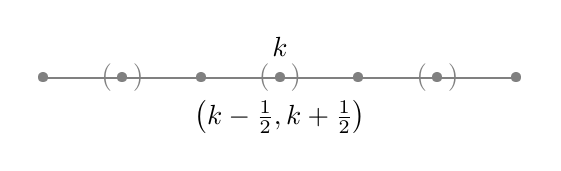
\begin{tikzpicture}
        \draw[gray] (-3,0) -- (3,0);
        \foreach \Point in {(-3, 0), (-2, 0), (-1, 0), (0, 0), (1, 0), (2, 0), (3, 0)}{
            \node[gray] at \Point {\textbullet};
        }
        \foreach \Point in {(-2.2, 0), (-0.2, 0), (1.8, 0)}{
            \node[gray] at \Point {$($};
        }
        \foreach \Point in {(-1.8, 0), (0.2, 0), (2.2, 0)}{
            \node[gray] at \Point {$)$};
        }
        \node at (0, 0.4) {$k$};
        \node at (0, -0.5) {$\left( k - \frac{1}{2}, k + \frac{1}{2} \right)$};
    \end{tikzpicture}
    \caption{\textit{Enteros en los reales como subespacio discreto.}}
    \label{fig:enteros-en-los-reales-como-subespacio-discreto.}
\end{figure}

    \item Si tomamos la topología del punto $(a \in X, \mathcal{T}_a|_{X \setminus \{a\}})$ vemos que se trata de la discreta.
\end{enumerate}
\end{ej}

\begin{obs}
\begin{enumerate}
    \item Los abiertos $W$ de un subespacio abierto $Y \ab X$ son abiertos en el espacio ambiente $X$.
   	$$
    W = U \cap Y : U,\ Y\ab X \Rightarrow W \ab X 
    $$
    \item Los cerrados $F$ de un subespacio cerrado $Y \cerr X$ son cerrados en el espacio ambiente $X$.
    $$
    F = C \cap Y : Y,\ C\cerr X \Rightarrow F \cerr X
    $$
\end{enumerate}
\end{obs}


\chapter{Aplicaciones continuas}%
\label{cha:aplicaciones_continuas}
Una vez vista la estructura de espacio topológico, nos encaminamos a estudiar los morfismos entre estructuras de este tipo. El primer paso para realizar este estudio es una característica clave, no sólo para el Análisis, sino  también para la Topología: la continuidad.

A partir de este capítulo, vamos a estudiar las buenas propiedades que adquieren las aplicaciones continuas por la forma en que transforman los abiertos entre espacios y relacionan las topologías de cada uno.

\section{Continuidad}%
\label{sec:continuidad}

Si hacemos memoria, recordaremos la famosa definición $\varepsilon-\delta$ para la continuidad que nos dieron para $\left( \mathbb{R}^n, \mathcal{T}_u \right)$. Esta venía decir que una función $f : X \rightarrow Y$ era continua en un punto $x_0\in X$ si y sólo si:
\[
\forall \varepsilon > 0, \ \exists \delta > 0 : \left(\lVert x - x_0 \rVert < \delta \Rightarrow \lVert f(x) - f(x_0) \rVert \right)
\]
y podemos reescribir esto último como $x \in B\left( x_0, \delta \right) \Rightarrow f\left( x \right) \in B\left( f\left( x_0 \right), \varepsilon \right)$ o también como $f\left( B\left( x_0, \delta \right) \right) \subset B\left( f\left( x_0 \right), \varepsilon \right) $. Lo anterior sugiere que la definición más ajena a las propiedades métricas y topológicas de $\mathbb{R}^n$ sería:
\[
\forall B\left( f\left( x_0 \right), \varepsilon \right),\ \exists B\left( x_0, \delta \right) \subset f^{-1}\left( B\left( f\left( x_0 \right), \varepsilon \right) \right)
\]
Sin embargo, esta definición sólo es válida para los espacios con la topología usual, pues el concepto de bola puede ser (y significar) cosas muy distintas en función de la topología empleada (sin ir más lejos puede no ser un abierto). Por ello, la siguiente definición pretende desligar el concepto de continuidad de la topología usual de $\mathbb{R}^n$ para que pueda ser aplicable a cualquier espacio topológico.

\begin{defi}[Continuidad]
Sea $f: X \rightarrow Y$ una función entre espacios topológicos, decimos que es \textbf{continua en $x_0$ $\in X$} si y sólo si:
\[
\forall V^{f\left( x_0 \right)} :  f^{-1}\left( V^{f\left( x_0 \right)} \right) = V^{x_0} 
\]
es decir, la preimagen de cualquier entorno de $f(x_0)$ es entorno de $x_0$.
\end{defi}

\begin{prop}[Composición de continuidades]
Sean $f:X \rightarrow Y$ y $g: Y \rightarrow Z$ funciones continuas en $x_0\in X$ e $y_0\in Y$ tales que $f(x_0) = y_0$, entonces la composición $h = g \circ f$ es una función continua en $x_0$.
\end{prop}
\begin{demo}
Escojamos un entorno $V^{h\left( x_0 \right)}$ de la imagen por $h$ de $x_0$, entonces
\[
h^{-1} V^{h\left( x_0 \right)} = f^{-1}g^{-1}V^{g\left( y_0 \right)} = f^{-1} V^{y_0} = V^{x_0}
\]
\end{demo}

\begin{ej}
\begin{enumerate}
    \item Sea $f: X_{\text{discreta}} \rightarrow Y$, entonces es continua sean cuales sean los conjuntos de partida y de llegada, pues todo es abierto y, en consecuencia, todo es entorno en $\mathcal{T}_{\text{disc}}$.
    \item Sea $f: X \rightarrow Y_{\text{trivial}}$, entonces es continua sean cuales sean los conjuntos de partida y de llegada, pues como $Y$ es el único abierto, entonces es el único entorno $V^{f\left( x \right)}$ para cualquier $f(x)$ y $f^{-1}V^{f\left( x \right)} = f^{-1}Y = X$, que es abierto.
    \item Si una función $f: X \rightarrow Y_{\text{discreta}}$ es continua, entonces $f$ es localmente constante, pues como en la trivial los puntos son abiertos, entonces el punto $\{f\left( x_0 \right)\}$ es entorno $V^{f\left( x_0 \right)}$ de sí mismo. Por tanto, por la continuidad de $f$, $f^{-1}f\left( x_0 \right) = V^{x_0}$, luego $f \equiv f\left( x_0 \right)$ en ese entorno $V^{x_0}$.
    \item Si una función $f: X \rightarrow Y$ es localmente constante, entonces es continua, puesto que si es localmente constante para cualquier $x_0 \in X$ existe un entorno $U^{x_0} : f\mid_{U^{x_0}} \equiv f\left( x_0 \right)$. De este modo, cualquier entorno $V^{f\left( x_0 \right)}$ de la imagen $f(x_0)$ cumple que $f^{-1}V^{f\left( x_0 \right)} \supset U^{x_0}$ y llamando $V^{x_0} = f^{-1} V^{f\left( x_0 \right)}$ entonces vemos que es entorno de $x_0$.
\end{enumerate}
\end{ej}

\begin{prop}[Caracterización de Continuidad]
Sea $f:X\rightarrow Y$ una función entre espacios topológicos, entonces son equivalentes:
\begin{enumerate}
    \item $f$ es continua.
    \item $\forall U \ab Y : f^{-1}\left( U \right) \ab X$.
    \item $\forall F \cerr Y : f^{-1}\left( F \right) \cerr X$.
    \item $\forall A \subset Y : f^{-1}\left( \mathring{A} \right) \subset \inter\left( f^{-1}\left( A \right) \right)$.
    \item $\forall A \subset X : f\left( \overline{A} \right) \subset \overline{f\left( A \right)}$.
\end{enumerate}
\end{prop}
\begin{demo}
\begin{itemize}
    \item $1. \Rightarrow 2.$
    
    Escojamos un abierto cualquiera $W \ab Y$. Por ser abierto, es entorno de todos sus puntos y, en particular, es entorno de las imágenes que puedan caer dentro de dicho abierto, es decir, $\forall x \in f^{-1} (W) : W = V^{f(x)}$. Por continuidad, las preimágenes de entornos de las imágenes son entornos de las preimágenes, luego $\forall x \in f^{-1} W : f^{-1}W = V^x$ y, como es entorno de todos sus puntos, entonces $f^{-1} W \ab X$.
    \item $2. \Rightarrow 3.$
    
    Como lo que sabemos es que las preimágenes de abiertos son abiertas y los cerrados se definen en términos de abiertos, no nos queda otra estrategia que intentar demostrarlo pasando los cerrados a sus complementarios: los abiertos.
    
    Escojamos un cerrado cualquiera $C \cerr Y$ de modo que conocemos que $Y \setminus C \ab Y$. Como conocemos el resultado para abiertos, podemos decir que $f^{-1}\left( Y\setminus C \right) \ab X$ y, conjuntistamente, $X \setminus f^{-1}C = f^{-1}\left( Y\setminus C \right)$, luego directamente tenemos que $f^{-1}C \cerr X$. 
    \item $3. \Rightarrow 5.$
    
    Como $\overline{f\left( A \right)} \cerr Y$ sabemos que $f^{-1}\overline{f\left( A \right)} \cerr X$. Como $A\subset f^{-1}f(A) \subset f^{-1}\overline{f\left( A \right)}$ y este último es cerrado en $X$, entonces $\overline{A}\subset f^{-1}\overline{f\left( A \right)}$ y, por tanto, $f\left( \overline{A} \right) \subset \overline{f\left( A \right)}$.
    \item $5. \Rightarrow 4.$
    \begin{gather*}
        Y \setminus \mathring{A}\Rightarrow \overline{Y\setminus A} \supset \overline{f\left( X \setminus f^{-1}A \right)} \stackrel{5)}{\supset} f\left( \overline{X \setminus f^{-1}\left( A \right)} \right) = f\left( X \setminus \inter\left( f^{-1}A \right) \right) \Rightarrow\\
        X \setminus \inter\left( f^{-1}A \right) \subset f^{-1}\left( Y\setminus \mathring{A} \right) = X \setminus f^{-1}\left( \mathring{A} \right)\Rightarrow f^{-1}\left( \mathring{A} \right) \subset \inter\left( f^{-1}A \right) 
    .\end{gather*}

    \item $4 \Rightarrow 1)$
    \begin{gather*}
        V^{f\left( x \right)} \Rightarrow f\left( x \right) \in \inter\left( V^{f\left( x \right)} \right) \Rightarrow x \in f^{-1}\left( \inter\left( V^{f\left( x \right)} \right) \right) \subset \inter\left( f^{-1}V^{f\left( x \right)} \right) \Rightarrow \\
        f^{-1}V^{f\left( x \right) } \text{ entorno de } x.
    \end{gather*}
\end{itemize}
\end{demo}

\begin{obs}
La definición y posterior caracterización nos permiten recuperar las propiedades de continuidad a las que estamos habituados, como por ejemplo el quinto apartado del que se desprende que la imagen del límite es el límite de la imagen, pero también nos da la posibilidad de utilizar dicha continuidad con fines meramente topológicos, como por ejemplo $id: \left( X, \mathcal{T}_1 \right) \rightarrow \left( X, \mathcal{T}_2 \right)$ es continua si y sólo si $\mathcal{T}_2 \subset \mathcal{T}_1$ (por 1).
\end{obs}

\section{Continuidad y subespacios}%
\label{sec:continuidad_y_subespacios}
En muchas ocasiones tiene interés estudiar el comportamiento de una función, no en el conjunto total, sino en un subconjunto de puntos concreto. Como hemos definido anteriormente los subespacios topológicos, tiene sentido querer ver cómo se comportan las aplicaciones y, sobre todo, la continuidad cuando trabajamos con estos subconjuntos.

\begin{prop}
Sea $f: X \rightarrow Y$ una función continua y $Z \subset X$ un subespacio topológico, entonces la restricción $f|_Z : Z \rightarrow Y$ también es continua.
\end{prop}
\begin{demo}
Aplicando la caracterización de continuidad a través de las preimágenes de abiertos, tenemos que:
\[
\forall A \ab Y : \left( f|_Z \right)^{-1} \left( A \right) = Z \cap f^{-1} A \ab Z
\]
donde este último conjunto es abierto por la definición de topología relativa.
\end{demo}

%TODO: Diagramas composición
\begin{obs}
\begin{enumerate}
    \item La aplicación inclusión $Z \stackrel{j}{\subset} X$ es continua.
    \begin{demo}
     Para cualquier abierto $U \ab X$ la preimagen $j^{-1}\left( U \right)$ corresponde a los puntos de $U \cap Z$, y este último conjunto es abierto en $Z$ por definición.
    \end{demo}

    \item La continuidad se hereda en la restricción a un subespacio, es decir, si consideramos la aplicación $Z \stackrel{j}{\subset} X \xrightarrow{f} Y$, entonces la continuidad de $f$ implica\footnote{Pero el recíproco no es cierto, la continuidad en un subespacio no extiende la continuidad a todo el espacio.} la continuidad de $f|_Z$.
    \begin{demo}
    Como $f|_Z = f \circ j$ y ambas son continuas, por composición, $f|_Z$ es continua.
    \end{demo}

    \item La continuidad es una propiedad local, es decir, que si $f|_{E^x}$ continua en $x$, entonces $f$ continua en $x$.
    \begin{demo}
	La preimagen de cualquier entorno $V^{f\left( x \right)}$ es $\left( f|_{E} \right)^{-1} \left( V^{f\left( x \right)} \right) = W^x$ un entorno de $x$ en $E^x$, pero tenemos que ver que lo es en $X$ para poder afirmar que es continua.
	Como $W^x \stackrel{\text{ent.}}{\subset} E^x \stackrel{\text{ent.}}{\subset} X$, entonces $W^x \stackrel{\text{ent.}}{\subset}X$, ya que entorno de entorno es entorno.
	
	Esta última afirmación es cierta porque:
        \begin{gather*}
        \begin{rcases}
           	W^x \stackrel{\text{ent.}}{\subset} E^x \Rightarrow \exists G \ab E^x \mbox{ tal que }G \subset W^x, \ G = A \cap E^x \subset X\\ 
            E^x \stackrel{\text{ent.}}{\subset} X \Rightarrow \exists B \ab X \mbox{ tal que } B \subset E^x
        \end{rcases}\Rightarrow\\
        x \in \underbrace{A \cap B}_{\ab X} \subset \underbrace{A \cap E^x}_{= G}  \subset W^x
        \end{gather*}
    \end{demo}

    \item Si $f|_{U \ab X}$ es continua $\Rightarrow f$ continua $\forall x \in U$.

    \item $x$ es aislado $\Rightarrow f$ continua en $x$. 
    \begin{demo}
        $x$ aislado $\Leftrightarrow V^x = \{x\}$ es abierto de $X$. $f|_{V^x} : \{x\} \rightarrow Y$.
    \end{demo}

    \item $f: X \rightarrow Y \supset Z$ tal que $f\left( X \right) \subset Z \subset Y$ (si no es así puede estar mal definido).

    Entonces, $f$ a $Y$ es continua $\Leftrightarrow f$ a $Z$ es continua.
    \begin{demo}
        \begin{itemize}
            \item $f$ cont. en $Z \xRightarrow{j \circ f} f$ cont. en $Y$. %TODO: Seguro?
            \item $f$ cont. en $Y \xRightarrow{?} f$ cont. en $Z$. 

            Sea $U_z$ ab. en $Z$. Este será $U_y \cap Z = U_z$ que cumple, $f_z^{-1}\left( U_y \cap Z \right) \stackrel{f\left( X \right) \subset Z}{=}  f_y^{-1}\left( U_y \right)$ que es abierto en $X$ (por ser $f_y$ continua).
        \end{itemize}
    \end{demo}
\end{enumerate}
\end{obs}

\begin{prop}[Criterios de continuidad por recubrimientos]
Sea $f: X \rightarrow Y$ una función entre espacios topológicos, si se da alguna de las siguientes condiciones: 
\begin{align*}
\begin{cases}
X = \bigcup_{i \in  I} U_i \mbox{ donde } U_i \ab X \\
\forall f|_{U_i} : U_i \rightarrow Y \mbox{ cont.}
\end{cases}
& &
\begin{cases}
X = \bigcup_{i =0}^n F_i \mbox{ donde } F_i \cerr X \\
\forall f|_{F_i} : F_i \rightarrow Y \mbox{ cont.}
\end{cases}
\end{align*}
entonces la función $f$ del inicio es continua.
\end{prop}
\begin{demo}
	\begin{itemize}
	\item Escojamos un abierto cualquiera $W \ab Y$ y veamos si su preimagen $f^{-1}W$ es un abierto en $X$.

    En primer lugar, por ser $X = \bigcup_{i \in  I} U_i$ podemos escribir que $f^{-1}W = X\cap f^{-1}W = \bigcup_{i \in  I} U_i \cap f^{-1} W = \bigcup_{i \in  I} \left( U_i \cap f^{-1} W\right) = \bigcup_{i \in  I} \left( f|_{U_i} \right)^{-1} W$. Como $\left( f|_{U_i} \right)^{-1}W \stackrel[\text{(cont.)}]{\text{ab.}}{\subset} U_i \ab X$, entonces $\left( f|_{U_i} \right)^{-1} W \ab X$ y de esta manera podemos escribir $f^{-1}W$ como unión de abiertos $\bigcup_{i \in  I} \left( f|_{U_i} \right)^{-1} W$ de $X$, es decir, que $f^{-1}W \ab X$.
	
	\item Escojamos un cerrado cualquiera $C \cerr Y$ y veamos si su preimagen $f^{-1}C$ es cerrada en $X$.

    En primer lugar, por ser $X = \bigcup_{i=0}^n F_i$ podemos escribir que $f^{-1}C = X\cap f^{-1}C = \bigcup_{i = 0}^n F_i \cap f^{-1} C = \bigcup_{i = 0}^n \left( F_i \cap f^{-1} C\right) = \bigcup_{i = 0}^n \left( f|_{F_i} \right)^{-1} C$. Como $\left( f|_{F_i} \right)^{-1}C \stackrel[\text{(cont.)}]{\text{cerr.}}{\subset} F_i \cerr X$, entonces $\left( f|_{U_i} \right)^{-1} C \cerr X$ y de esta manera podemos escribir $f^{-1}C$ como unión finita de cerrados $\bigcup_{i = 0}^n \left( f|_{F_i} \right)^{-1} C$ de $X$, es decir, que $f^{-1}C \cerr X$.
    \end{itemize}
\end{demo}


\section{Homeomorfismos}%
\label{sec:homeomorfismos}
Supongamos que tenemos una función $f$ biyectiva y continua. Con las definiciones de continuidad anteriores hemos caracterizado la topología de las imágenes por $f^{-1}$, pero no sabemos nada de cómo se comporta la función $f$ con respecto a abiertos, cerrados, etc.
Nos gustaría poder destacar en qué condiciones una función establece una biyección entre abiertos de dos espacios, pues de esa forma existiría un ``isomorfismo'' entre ambas topologías a la hora de trabajar con ellas. Esta idea es precisamente la que hay detrás de la definición de homeomorfismo.

\begin{defi}[Aplicaciones abiertas y cerradas]
Sea $f: X \rightarrow Y$ una función entre espacios topológicos, decimos que es:
\begin{itemize}
\item \textbf{abierta} si y sólo si las imágenes de abiertos son abiertos.
\item \textbf{cerrada} si y sólo si las imágenes de cerrados son cerrados.
\end{itemize}
\end{defi}

\begin{obs}
La caracterización que dimos de la continuidad hacía referencia a las preimágenes de abiertos y cerrados, no a sus imágenes. De hecho, ni la continuidad implica que la aplicación sea abierta o cerrada, ni viceversa.
\end{obs}

\begin{ej}
En la siguiente tabla podemos ver distintos ejemplos de funciones que verifican algunas de las condiciones que hemos definido, pero no otras simultáneamente:
\begin{table}[H]
\centering
\begin{tabular}{c|c|c|c}
Función & continua & abierta & cerrada \\
\hline
$Id: X_{\text{trivial}} \rightarrow X_{\text{discreta}}$ & \ding{55} & \checkmark & \checkmark \\
\hline
$Id: X_{\text{discreta}} \rightarrow X_{\text{trivial}}$ & \checkmark & \ding{55} & \ding{55} \\
\hline
$j: \left[ 0, 1 \right] \subset \mathbb{R}_{u}$ & \checkmark & \ding{55} & \checkmark \\
\hline
$j: \left( 0, 1 \right) \subset \mathbb{R}_u$ & \checkmark & \checkmark & \ding{55} \\
\hline
\end{tabular}
\caption{\textit{En la tabla anterior podemos ver ejemplos de funciones que son continuas, abiertas o cerradas de distintas formas.}}
\end{table}
\end{ej}

\begin{prop}[Trivialidades esenciales]
Sea $f:X\rightarrow Y$ una función biyectiva, entonces las siguientes afirmaciones son equivalentes:
\begin{enumerate}
    \item $f$ es abierta
    \item $f$ es cerrada
    \item $f^{-1}$ es continua.
\end{enumerate}
\end{prop}
\begin{demo}
\begin{itemize}
    \item $1. \Rightarrow 2.$
    
    Sea $F \cerr X$, por la definición de cerrado su complementario $X\setminus F$ es abierto en $X$. De esta manera, como $f$ es abierta, entonces $f\left( X\setminus F \right) \ab X$. Por la biyectividad, $f\left( X\setminus F \right) = Y\setminus f\left( F \right)$, es decir, que $f\left( F \right) \cerr Y$, lo que demuestra que $f$ es cerrada.

    \item $2. \Rightarrow 3.$
    
    Sea $F \cerr X$, como $f$ es cerrada, $f\left( F \right) \cerr Y$. Pero $f(F)= \left( f^{-1} \right)^{-1} \left( F \right)$ por la biyectividad de $f$, luego hemos demostrado que $f^{-1}$ continua porque las preimágenes de cerrados son cerrados.

    \item $3. \Rightarrow 1.$
    
    Sea $U \ab X$, por la continuidad de $f^{-1}$, la preimagen $\left( f^{-1} \right)^{-1} \left( U \right) \ab Y$. Por tanto, como $f\left( U \right) =  \left( f^{-1} \right)^{-1} \left( U \right)$, hemos demostrado que $f$ es abierta.
\end{itemize}
\end{demo}

\begin{defi}[Homeomorfismo]
Sea $f: X \rightarrow Y$ una aplicación biyectiva, decimos que es un \textbf{homeomorfismo} si y sólo si $f$ y $f^{-1}$ son continuas o, equivalentemente, si $f$ es continua y abierta o cerrada.
\end{defi}

\begin{obs}
La definición de homeomorfismo es importante porque no establece simples biyecciones entre conjuntos, establece biyecciones sobre topologías:
\begin{align*}
	f: \mathcal{T}_X &\rightarrow \mathcal{T}_Y\\
	U &\mapsto f\left( U \right)\\
	f^{-1}\left( W \right) &\mapsfrom W 
\end{align*}
Esto permite trabajar con los abiertos de un lado y trasladar el mismo trabajo a los del otro de forma canónica.
\end{obs}

\begin{defi}[Homeomorfismo Local]
Sea $f: X \rightarrow Y$ una función entre espacios topológicos, decimos que es un \textbf{homeomorfismo local en $x_0 \in X$} si y sólo si existen algunos entornos $V^{x_0}$ y $V^{f\left( x_0 \right)}$ tales que la restricción $f: V^{x_0} \rightarrow V^{f\left( x_0 \right)}$ es un homeomorfismo.
\end{defi}

\begin{obs}
En general, cuando decimos que una aplicación $f:X\rightarrow Y$ es un homeomorfismo local sin especificar en qué punto, estamos diciendo que es homeomorfismo local para cualquier punto $x\in X$.
\end{obs}

\begin{obs}
En la definición de homeomorfismo local anterior, podemos tomar $V^{x_0}$ y $V^{f\left( x_0 \right)}$ como entornos abiertos.
%TODO: Habría que meter un diagrama de flechas como el que hizo en clase (preguntar a JD por él si no lo encontramos)
\begin{demo}
Si $f$ es homeomorfismo local, entonces $\exists V^a \subset X$ y $V^{f\left( a \right)} \subset Y$ tal que $f: V^a \rightarrow V^{f\left( a \right)}$ es homeomorfismo y, por esta razón, sabemos que $\exists U^a \ab V^a$ tal que $f\left( U^a \right) \ab V^{f\left( a \right)}$. 

Además, como $f(U^a)$ es abierto en $V^{f\left( a \right)}$, sabemos que $f(U^a)$ es entorno\footnote{En este punto no podemos parar y decir que es abierto porque lo que sabemos es que $f(U^a)$ es abierto en $V^{f(a)}$, pero no sabemos nada sobre si es abierto en $Y$, que es lo que necesitamos.} de $f(a)$ en $V^{f(a)}$. Como tenemos la secuencia $f(U^a) \ent V^{f(a)} \ent Y$, sabemos que $f(U^a) \ent Y$ de $f(a)$ y, por tanto, podemos encontrar un abierto $W \ab Y$ tal que $W\subset f(U^a)$.

Por tanto, como se trata de un homeomorfismo local, existirá algún $G \ab U^a$ de forma que $f(G) = W$. Pero como $U^a$ es abierto global, entonces tenemos que $G\ab X$ y hemos acabado, pues tenemos el homeomorfismo local definido en $f: G \rightarrow W$.
\end{demo}
\end{obs}

\begin{prop}[Restricción de homeomorfismos]
Sea $f: X \rightarrow Y$ un homeomorfismo, la restricción $f: Z \rightarrow f\left( Z \right)$ a cualquier subespacio $Z \subset X$ también es homeomorfismo.
\end{prop}
\begin{demo}
La restricción será biyectiva por serlo $f$ y ser el conjunto de llegada $f(Z)$. Una biyección es homeomorfismo si tanto $f$ como $f^{-1}$ son continuas y como ya vimos que la restricción de una continua es continua, sabemos que la restricción de $f$ y $f^{-1}$ a $Z$ y $f\left( Z \right)$ son también continuas, es decir, $f|_Z$ es homeomorfismo.
\end{demo}

\begin{prop}[Composición de homeomorfismos]
Sean $f: X \rightarrow Y$ y $g: Y \rightarrow Z$ dos homeomorfismos, su composición $h = f \circ g$ también es homeomorfismo.
\end{prop}

\begin{prop}
Sea $f:X\rightarrow Y$ un homeomorfismo local, entonces es abierto.
\end{prop}
\begin{demo}
Hay dos formas de demostrarlo, la primera es intentando ver que para cualquier $U \ab X$ ocurre que $f\left( U \right)$ es entorno de las imágenes de todos los puntos de $U$.

Con este objetivo, sabemos que por ser $f$ homeomorfismo local existe una restricción $\exists f| : V^{x_0} \rightarrow V^{y_0}$ para cada punto $x_0\in U$ y usando la notación $y_0 = f(x_0)$. Como esta restricción es homeomorfismo, $f\left( U \cap V^{x_0} \right) \ab V^{y_0}$ y, por tanto, $ f \left( U \cap V^{x_0} \right)$ es entorno en $Y$ de $y_0$. Al ocurrir esto para todos los puntos y, teniendo en cuenta que $f \left( U \cap V^{x_0} \right)\subset f(U)$, sabemos que $f(U)$ es entorno de las imágenes de todos los puntos de $U$.

La otra forma de verlo es que, por ser homeomorfismo local, para cualquier punto $x\in X$ existe un entorno abierto $W^x \ab X$ de forma que $f(W^x)\ab Y$ es abierto. De esta manera, y abusando de la notación, escribiendo $W^x = W^x \cap U$, $U$ puede expresarse como $U = \bigcup_{x\in U} W^x$. Por tanto, $f(U) = f(\bigcup_{x\in U} W^x) = \bigcup_{x\in U} f(W^x)$ que es unión de abiertos, luego es abierto.
\end{demo}

% TODO: estos ejemplos hay que mirarlos despacio y corregirlos
\begin{ej}[¡Importantes!]
\begin{enumerate}
    \item \textbf{Proyección estereográfica}:

    Sea $\mathbb{S}^m$ y $a \in \mathbb{S}^m \Rightarrow \mathbb{S}^{m} \setminus \{a\} \rightarrow \mathbb{R}^m$ homeomorfismo. ($\mathbb{R}^{m}$ es en realidad un hiperplano de $\mathbb{R}^{m+1}$ en el que se encuentra contenida la ``esfera'')

    \item \textbf{Proyección exponencial}: 

    $\mathbb{R} \rightarrow \mathbb{S}^1: \theta \mapsto e^{2\pi i\theta} = \left( \cos 2\pi \theta, \sin 2\pi \theta \right)$ es homeomorfismo local, pero no es inyectiva al ser periódica.

    \item \textbf{Proyección antipodal}:

    $\mathbb{R}^{m+1}\setminus \{0\} \supset \mathbb{S}^m \rightarrow \mathbb{R}\mathrm{P}^{m}: x \mapsto \left[ x \right]$ es homeomorfismo local. Es 2-1 por llevar las antípodas al mismo $\left[ x \right]$. 

    Podemos dividir $\mathbb{S}^{m}$ tal que: $\mathbb{S}^{m} = S_{+} \cup S_{-} \cup E$ (ecuador). Llamando $U_p$ a todas las rectas no contenidas en el plano ortogonal a la recta formada por el punto que se quita y su antípoda. Con esto tenemos $U_p \simeq \mathbb{R}^{m}$. Uniéndolo con el hiperplano del infinito $H_p^{\infty}$ tenemos que los polos van a $U_p$ y $E$ a $H_p^{\infty}$. Esta correspondencia es homeomorfa por lo que se puede trasladar la topología.

    Con esto, esta proyección será un recubrimiento doble de $\mathbb{R}\mathrm{P}^m,\ m \ge 2$.

    \item \textbf{Lemniscata}:

    $f: \mathbb{R} \rightarrow X \subset \mathbb{R}^2: t \mapsto \left( \frac{t}{1 + t^4}, \frac{t^3}{1 + t^4} \right)$ es biyectiva y continua, pero NO homeomorfismo local.
    \begin{figure}[H]
        \centering
        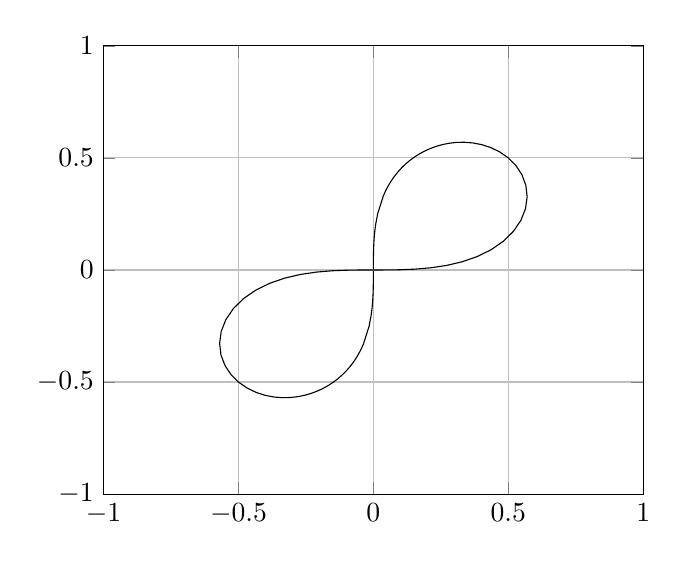
\begin{tikzpicture}
            \begin{axis}[
                xmin=-1,xmax=1,
                ymin=-1,ymax=1,
                grid=both,
                ]
                %TODO: Aumentar el tamaño para la versión final
                %Ponemos varios intervalos para minimizar las samples y, por tanto, el tiempo de compilación.
                \addplot [domain=-3:3,samples=100]({(x/(1+x^4))},{(x^3/(1+x^4))}); 
                \addplot [domain=-3:-50,samples=50]({(x/(1+x^4))},{(x^3/(1+x^4))}); 
                \addplot [domain=-50:-200,samples=50]({(x/(1+x^4))},{(x^3/(1+x^4))}); 
                \addplot [domain=3:50,samples=50]({(x/(1+x^4))},{(x^3/(1+x^4))}); 
                \addplot [domain=50:200,samples=50]({(x/(1+x^4))},{(x^3/(1+x^4))}); 
            \end{axis}
        \end{tikzpicture}
        \caption{\textit{Representación Lemniscata.}}
        \label{fig:lemniscata}
    \end{figure}

    Engañosamente: 
    \[
        \forall t \in \mathbb{R},\ \exists \left( t - \varepsilon, t + \varepsilon \right) = I_{\varepsilon}: f| : I_{\varepsilon} \rightarrow f\left( I_{\varepsilon} \right) 
    \]
    es homeomorfismo.

    En $t = 0,\ f\left( I_{\varepsilon} \right)$ NO es entorno de $f\left( 0 \right) = \left( 0, 0 \right)$, porque se tienen que tomar elementos de la rama ``vertical''.

    \item Las \textbf{coordenadas polares} $\left( 0, \rightarrow \right) \times \mathbb{R}^{} \rightarrow \mathbb{R}^{2},\ \left( r, \theta \right) \mapsto \left( r\cos \theta, r \sin \theta \right)$ son homeomorfismo local con $\theta_0 \in \left( \theta_0 - \pi, \theta_0 + \pi \right)$ hasta $\mathbb{R}^{2} \setminus L$ con $L$ la recta entre $O$ y $\theta_0$.
\end{enumerate} 
\end{ej}

\begin{defi}[Variedad Topológica]
Una \textbf{variedad topológica} de dimensión $m$ es un espacio localmente homeomorfo a $\mathbb{R}^m$, es decir, que cada punto tiene un entorno abierto homeomorfo a una bola\footnote{Luego, en el fondo, es homeomorfo a cualquier bola y, por ser éstas parte de una base de $\mathbb{R}^m$, es homeomorfo a todo $\mathbb{R}^m$.} $B\left( 0, \varepsilon \right) \subset \mathbb{R}^m$.
\end{defi}
\begin{ej}
Esferas, espacios proyectivos, toros...
\end{ej}


\chapter{Construcciones}%
\label{cha:construcciones}
En este capítulo buscaremos topologías en base a unas aplicaciones con el objetivo de hacer a dichas aplicaciones continuas. Tras esto, daremos una caracterización de la topología construida. Por último, exploraremos las propiedades de las construcciones.

\section{Imágenes inversas}%
\label{sec:imagenes_inversas}
El objetivo de esta construcción es crear una topología que, al ser equipada en el conjunto de partida, haga la aplicación $f: (Y, ?) \rightarrow \left( X, \mathcal{T} \right)$ continua. Recordemos que, para poder cumplir con la definición de continuidad, las preimágenes de abiertos deben ser abiertos, luego cuantos más abiertos ``metamos'' en dicha topología más ``fácil'' será que las imágenes inversas caigan en abiertos.

Con dicha observación lo que se nos viene a la cabeza es tomar como topología la discreta, sin embargo, esto carece de interés: lo que realmente nos gustaría es la topología con menos abiertos posibles que haga la función continua.

\begin{defi}[Topología Imagen Inversa]
Sea $f: Y \rightarrow (X,\mathcal{T})$ una aplicación, definimos la \textbf{topología de la imagen inversa} como la topología menos fina que podemos equipar a $Y$ para que la aplicación $f$ sea continua, que es la topología:
$$
f^{-1} \mathcal{T} = \{f^{-1}U: U \in \mathcal{T}\}
$$
donde los abiertos son exactamente las preimágenes de los abiertos la topología de llegada.
\end{defi}

\begin{obs}
Tras la introducción de la sección, la topología de la definición parece la más razonable para ser candidata a menos fina posible, puesto que de ser topología (hay que probarlo) hemos ``metido'' los abiertos indispensables para la continuidad que son precisamente las imágenes inversas.
\end{obs}

\begin{prop}
Sea $f: (Y, f^{-1}\mathcal{T}) \rightarrow (X,\mathcal{T})$ donde $f^{-1}\mathcal{T}$ es la topología de la imagen inversa, entonces:
\begin{enumerate}
    \item $f^{-1}\mathcal{T}$ es topología. 
    \item $f^{-1}\mathcal{T}$ es la menos fina posible.
\end{enumerate}
\end{prop}
\begin{demo}
\begin{enumerate}
    \item Las imágenes inversas funcionan muy bien con uniones, intersecciones, etc. Por tanto, la demostración de que es topología es trivial.
    
    \item Consideremos cualquier otra topología $\mathcal{T}'$ en $Y$ que haga la función $f$ continua. Si tomamos un abierto $U \in f^{-1}\mathcal{T}$ en la topología inversa, entonces $\exists V \in \mathcal{T}: f^{-1}V = U$. Asimismo, como $f$ también es continua en $\mathcal{T}'$ sabemos que $U = f^{-1}V$ también es abierto en $\mathcal{T}'$, es decir, todo abierto en $f^{-1}\mathcal{T}$ es también abierto en $\mathcal{T}'$ y, por tanto, $f^{-1}\mathcal{T} \subset \mathcal{T}'$.
\end{enumerate}
\end{demo}

\subsection{Caracterización de la imagen inversa}
\label{sub:caracterizacion_de_la_imagen_inversa}
En muchas ocasiones, tendremos diagramas con varias aplicaciones entre varios espacios topológicos. En estas situaciones, es de utilidad tener algún teorema para poder identificar unas topologías con otras, ya que entender y manejar bien unas pueden tener buenas ``traslaciones'' en las otras. Es por ello que tiene gran utilidad el siguiente teorema de caracterización de la topología inversa en circunstancias como las descritas.

\begin{theo}[Propiedad universal de las inmersiones]
Sean $g: \left( Z, \mathcal{T}'' \right) \rightarrow \left( Y, \mathcal{T}' \right)$ y $f: \left( Y, \mathcal{T}' \right) \rightarrow \left( Z, \mathcal{T} \right)$ dos funciones entre espacios topológicos:
\begin{figure}[H]
        \centering    
            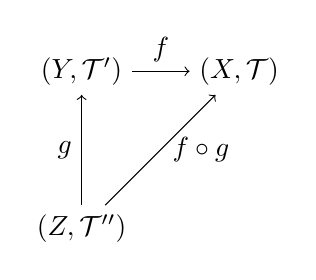
\begin{tikzpicture}[node distance=2cm, auto]
            \node(Y) {$\left( Y, \mathcal{T}' \right)$};
            \node(X) [right of=Y] {$\left( X, \mathcal{T} \right)$};
            \node(Z) [below of=Y] {$\left( Z, \mathcal{T}'' \right)$};
            \draw[->](Y) to node {$f$}(X);
            \draw[->](Z) to node [left] {$g$}(Y);
            \draw[->](Z) to node [right=0.2ex] {$f \circ g$}(X);
            \end{tikzpicture}
        \caption{\textit{Ilustración de la composición propuesta}}
        \label{prop_universal_inmersiones}
    \end{figure}
entonces $\mathcal{T}' = f^{-1}\mathcal{T}$ si y sólo si:
\[
\forall g: g \text{ cont.} \Leftrightarrow f \circ g \text{ cont.}
\]    
\end{theo}
\begin{demo}
\begin{itemize}
    \item $\Rightarrow)$ $\mathcal{T}' = f^{-1}\mathcal{T}: $ 
    \begin{itemize}
        \item $g$ cont. $\Rightarrow f \circ g$ cont. es trivial por composición de continuas.
        \item $f \circ g$ cont. $\Rightarrow g$ cont.
        
        Para probarlo, basta ver para cualquier abierto $V \in \mathcal{T}'$, $g^{-1}V$ es abierto en $\mathcal{T}''$. Por ser $\mathcal{T}'=f^{-1}\mathcal{T}$, entonces $g^{-1}V = g^{-1} f^{-1} U$ para algún abierto $U\in \mathcal{T}$, pero es que precisamente $g^{-1} f^{-1} U = \left( f \circ g \right)^{-1} U \in \mathcal{T}''$ por ser $f\circ g$ continua.
    \end{itemize}

    \item $\Leftarrow)$
	Para demostrarla vamos a ver el doble contenido de $\mathcal{T}'$ en $f^{-1}\mathcal{T} $ y viceversa.
	
	Como la propiedad de caracterización se cumple para cualquier $g$ que escojamos, podemos escoger como $g$ la aplicación identidad. De esta manera, $g \text{ cont.} \Leftrightarrow f\circ g \text{ cont.}$ implica que $id \text{ cont.} \Leftrightarrow f\circ id = f \text{ cont.}$, luego hemos demostrado que $f$ es continua.
    \begin{figure}[H]
        \centering    
            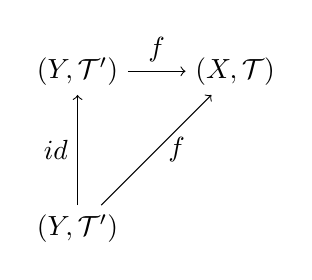
\begin{tikzpicture}[node distance=2cm, auto]
            \node(Y) {$\left( Y, \mathcal{T}' \right)$};
            \node(X) [right of=Y] {$\left( X, \mathcal{T} \right)$};
            \node(Z) [below of=Y] {$\left( Y, \mathcal{T}' \right)$};
            \draw[->](Y) to node {$f$}(X);
            \draw[->](Z) to node [left] {$id$}(Y);
            \draw[->](Z) to node [right=0.2ex] {$f$}(X);
            \end{tikzpicture}
    \end{figure}
    Y como precisamente $f^{-1}\mathcal{T}$ es la topología menos fina que posibilita la continuidad de $f$, sabemos que $\mathcal{T}' \supset f^{-1}\mathcal{T}$. 
   
   Si ahora utilizamos como $g$ la identidad puramente conjuntista (las topologías no se conservan, pero los puntos van a ellos mismos), entonces:
    \begin{figure}[H]
        \centering    
            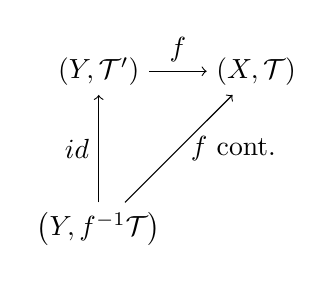
\begin{tikzpicture}[node distance=2cm, auto]
            \node(Y) {$\left( Y, \mathcal{T}' \right)$};
            \node(X) [right of=Y] {$\left( X, \mathcal{T} \right)$};
            \node(Z) [below of=Y] {$\left( Y, f^{-1}\mathcal{T} \right)$};
            \draw[->](Y) to node {$f$}(X);
            \draw[->](Z) to node [left] {$id$}(Y);
            \draw[->](Z) to node [right=0.2ex] {$f$ cont.}(X);
            \end{tikzpicture}
    \end{figure}
    de nuevo, por la propiedad de caracterización sabemos que esta nueva ``identidad'' es una función continua. Como la aplicación es entre el mismo conjunto de puntos es biyectiva, entonces cualquier abierto $U\in \mathcal{T}'$ coincide con su preimagen $f^{-1}U$. Al demostrar que la ``identidad'' es continua, entonces $\forall U \in \mathcal{T}', \ U = f^{-1}U\in f^{-1}\mathcal{T}$, es decir, que $\mathcal{T}'\subset f^{-1}\mathcal{T}$.
\end{itemize}
\end{demo}

\subsection{Inmersiones}
\label{sub:inmersiones}
La construcción anterior cobra especial relevancia cuando la aplicación $f: Y \rightarrow X$ que hemos hecho continua con la topología imagen inversa es inyectiva porque de alguna forma permite ``sumergir'' el espacio de salida en el de llegada.

\begin{defi}[Inmersión]
Sea $f:\left( Y, f^{-1}\mathcal{T} \right) \rightarrow \left( X, \mathcal{T} \right)$ una aplicación continua gracias a la topología de la imagen inversa, decimos que es una \textbf{inmersión} si y sólo si es inyectiva.
\end{defi}

\begin{prop}[Caracterización de Inmersiones]
Sea $f: \left( Y, \mathcal{T}' \right) \rightarrow \left( X, \mathcal{T} \right)$ una aplicación entre espacios topológicos, entonces:
\[
    f\text{ es inmersión} \Leftrightarrow f: \left( Y, \mathcal{T}' \right) \xrightarrow{\text{homeo.}} \left( f\left( Y \right), \mathcal{T}|_{f\left( Y \right)} \right)
\]
\end{prop}
\begin{demo}
\begin{itemize}
    \item $\Rightarrow)$ Tenemos que $f: \left( Y, f^{-1}\mathcal{T} \right) \rightarrow \left( f\left( Y \right), \mathcal{T}|_{f\left( Y \right)} \right)$. 

    Como $f$ es inmersión sabemos que es inyectiva, lo que sumado a que el espacio de llegada es $f(Y)$, nos permite saber que es sobreyectiva y, por tanto, biyectiva. De los requisitos para ver que es un homeomorfismo, bastaría con ver que es abierta y continua:
    \begin{itemize}
        \item Continua:
        
        Si escogemos un abierto cualquier $U\in \mathcal{T}\mid_{f(Y)}$, por ser abierto de la topología relativa, sabemos que $\exists W \in \mathcal{T}: U = f\left( Y \right) \cap W $ y entonces su imagen inversa
        \[
        f^{-1}\left( U \right) = f^{-1}\left( W \cap f\left( Y \right) \right) = Y \cap f^{-1}\left( W \right) = f^{-1}\left( W \right) \in f^{-1}\mathcal{T}
        \]

        \item Abierta:
        
        Observamos que cualquier abierto $U \in f^{-1}\mathcal{T}$ de la topología imagen inversa es preeimagen de un abierto de la topología de llegada, es decir, $\exists W \in \mathcal{T}: f^{-1}W = U$. Por tanto, si calculamos la imagen de $U$ por $f$, tenemos que:
        \[
        fU = ff^{-1}W = W \cap f\left( Y \right) \ab f\left( Y \right)
        \]
        es decir que $fU$ es abierto en $f\left( Y \right)$.
    \end{itemize}

    %TODO: Posiblemente mal. Algo de la relativa 
    \item $\Leftarrow)$ Veamos por el doble contenido que $\mathcal{T}' = f^{-1}\mathcal{T}$
    \begin{itemize}
        \item $\subset)$
        
        Sea $U \in \mathcal{T}'$, como es homeomorfismo es abierto, luego $fU\in \mathcal{T}|_{f\left( Y \right)}$, es decir, $\exists W \in \mathcal{T}'|_{f\left( Y \right)}: f^{-1}W = U$, luego podemos decir que $U \in f^{-1}\mathcal{T}$. 
        \item $\supset)$
        
        Sea $U \in f^{-1}\mathcal{T}$, por definición, $\exists W \in \mathcal{T}|_{f\left( Y \right)}: f^{-1}W = U$ y, como $f$ es continua en $\mathcal{T}'$, $U = f^{-1} W \in \mathcal{T}'$.
    \end{itemize}
\end{itemize} 
\end{demo}

\begin{obs}
Podemos extraer de la definición, pero sobre todo de la caracterización anterior de inmersión las siguientes conclusiones:
\begin{enumerate}
    \item Si una función $f: Y \rightarrow X$ es inyectiva, continua y abierta o cerrada, entonces es inmersión.
    \begin{demo}
    La caracterización de imagen inversa exige continuidad, biyectividad y apertura o cierre (es decir, que sea homeomorfismo) de la aplicación $g: Y \rightarrow f(Y)$. Como $f$ es inyectiva y coincide con $g$ en la imagen $f(Y)$, ésta última también es inyectiva, luego por ser sobreyectiva es biyectiva. La continuidad también se extiende a $g$ naturalmente y falta solo ver que es abierta o cerrada respectivamente. Si $f$ lo es, entonces para cualquier abierto o cerrado $W\subset Y$ su imagen $f(W)$ será abierta o cerrada en $X$. Del mismo modo, para cualquier abierto o cerrado $W\subset Y$ su imagen $g(W)$ se puede escribir como $g(W) = f(W)\cap f(Y)$ que es abierto o cerrado por ser un corte de un abierto o cerrado ambiente con el subespacio $f(Y)$.
    \end{demo}

    \item Si $f: Y \rightarrow X$ es una inmersión, entonces:
	\begin{itemize}
		\item es una aplicación abierta si y sólo si 	$f(Y)$ es abierto en $X$.
		\item es una aplicación cerrada si y sólo si $f(Y)$ es cerrado en $X$.
	\end{itemize}	    
    
    \begin{demo}
    En ambos casos, la implicación de izquierda a derecha es trivial, luego sólo es necesaria la de derecha a izquierda:
    \begin{itemize}
        \item 
        $\forall V = f^{-1}U \in f^{-1}\mathcal{T}, \ fV = \overbrace{U \cap f\left( Y \right)}^{\text{inter. abiertos}} \in \mathcal{T}$.
        \item 
        $\forall C \cerr  f^{-1}\mathcal{T}, \ Y\setminus C = f^{-1} U \in f^{-1}\mathcal{T} \Rightarrow f\left( C \right) = \underbrace{\left( X\setminus U \right) \cap f\left( Y \right)}_{\text{inter. cerrados}}  \cerr X$ 
    \end{itemize} 
    \end{demo}

    \item Las inmersiones y la apertura o cierre de la aplicación no están relacionadas. Esto quiere decir que existen inmersiones que no son abiertas ni cerradas, que sólo son abiertas, que sólo son cerradas y ambas cosas simultáneamente.
\end{enumerate}
\end{obs}

\begin{obs}
Las inmersiones son las que justifican la idea de considerar unos espacios como subespacios de otros. Las frases ``el plano proyectivo real no es un subespacio de $\mathbb{R}^3$'', ``la esfera no es un subespacio de $\mathbb{R}^2$'' o ``el plano proyectivo real es un subespacio de $\mathbb{R}^4$'' se refieren a esto mismo: cuándo hay o no hay una inmersión del primer espacio en el segundo, es decir, un subespacio del segundo homeomorfo al primero.
\end{obs}

\section{Imágenes directas}%
\label{sec:imagenes_directas}
El objetivo de esta construcción es crear una topología que, al ser equipada en el conjunto de llegada, haga la aplicación $f: (X, \mathcal{T}) \rightarrow \left( Y, ? \right)$ continua. De nuevo, recordemos que, para poder cumplir con la definición de continuidad, las preimágenes de abiertos deben ser abiertos, luego cuantos menos abiertos ``metamos'' en dicha topología menos posibilidades habrá de que sus preimágenes no caigan en abiertos.

Con dicha observación, en este caso lo que se nos viene a la cabeza es tomar como topología la trivial, sin embargo, esto vuelve a carecer de interés: lo que realmente nos gustaría es la topología con más abiertos posibles que haga la función continua.

\begin{defi}[Topología Imagen Directa]
Sea $f: (X,\mathcal{T}) \rightarrow Y$ una aplicación, definimos la \textbf{topología de la imagen directa} como la topología más fina que podemos equipar a $Y$ para que la aplicación $f$ sea continua, que es la topología:
$$
f \mathcal{T} = \{V \subset Y: f^{-1}V \in \mathcal{T}\}
$$
donde los abiertos son exactamente aquellos cuyas preimágenes son abiertos de la topología de salida.
\end{defi}

\begin{obs}
Tras la introducción de la sección, de nuevo, parece que la topología de la definición es la más razonable para ser candidata a más fina posible, puesto que de ser topología (hay que probarlo) hemos ``metido'' todo lo que podemos meter como abierto conservando el requisito de la continuidad.
\end{obs}

\begin{prop}
Sea $f: (X,\mathcal{T}) \rightarrow (Y, f\mathcal{T})$ donde $f\mathcal{T}$ es la topología de la imagen directa, entonces:
\begin{enumerate}
    \item $f\mathcal{T}$ es topología. 
    \item $f\mathcal{T}$ es la más fina posible.
\end{enumerate}
\end{prop}

\begin{demo}
\begin{enumerate}
    \item Trivial.
    \item Consideremos cualquier otra topología $\mathcal{T}'$ en $Y$ tal que haga $f$ continua. Si tomamos un abierto $U \in \mathcal{T}'$, como conserva la continuidad , $f^{-1} U = W \in \mathcal{T}$. Sin embargo, tal y como hemos definido $f \mathcal{T}$, sabemos que $U \in f \mathcal{T}$ porque $W \ab X$, luego $\mathcal{T}'\subset f\mathcal{T}$.
\end{enumerate}
\end{demo}

\subsection{Caracterización de la imagen directa}
\label{sub:caracterizacion_de_la_imagen_directa}
De nuevo, en las situaciones en las que haya diagramas con varias aplicaciones entre varios espacios topológicos, es de utilidad tener algún teorema para poder identificar unas topologías con otras, ya que entender y manejar bien unas pueden tener buenas ``traslaciones'' en las otras. Por ello, tiene gran utilidad el teorema de caracterización de la topología directa en circunstancias como las descritas.

\begin{theo}[Propiedad universal de las identificaciones]
Sean $g: \left( Y, \mathcal{T}' \right) \rightarrow \left( Z, \mathcal{T}'' \right)$ y $f: \left( X, \mathcal{T} \right) \rightarrow \left( Y, \mathcal{T}' \right)$ dos funciones entre espacio topológicos
    \begin{figure}[H]
        \centering    
            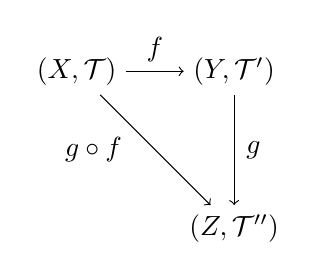
\begin{tikzpicture}[node distance=2cm, auto]
            \node(X) {$\left( X, \mathcal{T} \right)$};
            \node(Y) [right of=X] {$\left( Y, \mathcal{T}' \right)$};
            \node(Z) [below of=Y] {$\left( Z, \mathcal{T}'' \right)$};
            \draw[->](X) to node {$f$}(Y);
            \draw[->](X) to node [left=0.3cm] {$g \circ f$}(Z);
            \draw[->](Y) to node [right=0.2ex] {$g$}(Z);
            \end{tikzpicture}
        \caption{\textit{Ilustración de la composición propuesta}}
        \label{prop_universal_directas}
    \end{figure}
entonces $\mathcal{T}' = f\mathcal{T}$ si y sólo si:
	\[
        \forall g, \ g \text{ cont.} \Leftrightarrow g \circ f \text{ cont.}
	\]
\end{theo}
\begin{demo}
\begin{itemize}
    \item $\Rightarrow)$ $\mathcal{T}' = f\mathcal{T}: $ 
    \begin{itemize}
        \item $g$ cont. $\Rightarrow g \circ f$ cont. es trivial por composición de continuas.
        \item $g \circ f$ cont. $\Rightarrow g$ cont.
        
        Si escogemos un $W \in \mathcal{T}''$ sabemos que $f^{-1}\left( g^{-1} W \right) = \left( g \circ f \right)^{-1} W \in \mathcal{T}$ porque la aplicación $g\circ f$ es continua. Sin embargo, que $f^{-1} V \in \mathcal{T}$ implica que $V\in \mathcal{T}'$ porque $\mathcal{T}' = f\mathcal{T}$, luego $g^{-1}W \in \mathcal{T}'$, es decir, es continua.
    \end{itemize}

    \item $\Leftarrow)$
    Para demostrarla vamos a ver el doble contenido de $\mathcal{T}'$ en $f^{-1}\mathcal{T} $ y viceversa.
    
    Como la caracterización se cumple para cualquier $g$, en particular podemos seleccionar como $g$ la identidad. Como la identidad es continua, por la caracterización, $id \circ f = f$ es continua y, como $f\mathcal{T}$ es la topología más fina que hace $f$ continua, entonces $\mathcal{T}'\subset f\mathcal{T}$.

    \begin{figure}[H]
        \centering    
            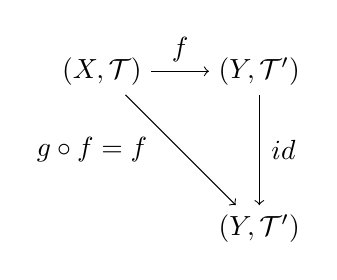
\begin{tikzpicture}[node distance=2cm, auto]
            \node(X) {$\left( X, \mathcal{T} \right)$};
            \node(Y) [right of=X] {$\left( Y, \mathcal{T}' \right)$};
            \node(Z) [below of=Y] {$\left( Y, \mathcal{T}' \right)$};
            \draw[->](X) to node {$f$}(Y);
            \draw[->](X) to node [left=0.3cm] {$g \circ f = f$}(Z);
            \draw[->](Y) to node [right=0.2ex] {$id$}(Z);
            \end{tikzpicture}
    \end{figure}
    
    De la misma manera que antes, podemos seleccionar como $g$ la identidad meramente conjuntista (donde cada punto va a sí mismo, pero no se conserva la topología porque son distintas la de salida y la de llegada). 
    \begin{figure}[H]
        \centering    
            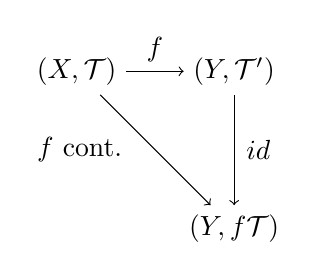
\begin{tikzpicture}[node distance=2cm, auto]
            \node(X) {$\left( X, \mathcal{T} \right)$};
            \node(Y) [right of=X] {$\left( Y, \mathcal{T}' \right)$};
            \node(Z) [below of=Y] {$\left( Y, f\mathcal{T} \right)$};
            \draw[->](X) to node {$f$}(Y);
            \draw[->](X) to node [left=0.3cm] {$f$ cont.}(Z);
            \draw[->](Y) to node [right=0.2ex] {$id$}(Z);
            \end{tikzpicture}
    \end{figure}
	En este caso, como $f$ va de $(X,\mathcal{T})$ a $(Y, f\mathcal{T})$ es continua por definición de $f\mathcal{T}$ y, por la caracterización, sabemos que la ``identidad'' que hemos seleccionado también lo es. Esto quiere decir que $\forall W \in f\mathcal{T}, id^{-1} W = W \in \mathcal{T}'$, por tanto, $f\mathcal{T}\subset \mathcal{T}'$.
\end{itemize}
\end{demo}

\begin{obs}
$f\left( X \right)$ es abierto y cerrado en $f\mathcal{T}: \begin{cases}
    \forall y \in Y \setminus f\left( X \right), f^{-1}y = \emptyset \in \mathcal{T} \Rightarrow \{y\} \in f\mathcal{T}\\
    f^{-1}f\left( X \right) = X \in \mathcal{T} \Rightarrow f\left( X \right) \in f\mathcal{T}
\end{cases}$
\end{obs}

%TODO: En sus apuntes el orden es distinto a como lo dio en clase. De momento, lo dejo como en los apuntes.
\subsection{Identificaciones}
\label{sub:identificaciones}
La construcción anterior cobra especial relevancia cuando la aplicación $f: Y \rightarrow X$ que hemos hecho continua con la topología imagen directa es sobreyectiva porque de alguna forma permite ``identificar'' el espacio de llegada en el de salida.

\begin{defi}[Identificación]
Sea $f: \left( X, \mathcal{T} \right) \rightarrow \left( Y, \mathcal{T}' \right)$ una aplicación sobreyectiva, decimos que es una \textbf{identificación} si y sólo si $\mathcal{T}' = f\mathcal{T}$.
\end{defi}

\begin{obs}
\begin{enumerate}
    \item Las identificaciones verifican $V \stackrel{\text{ab}}{\subset} Y \Leftrightarrow f^{-1}V \stackrel{\text{ab}}{\subset} X$ y la continuidad $V \stackrel{\text{ab}}{\subset } Y \Rightarrow f^{-1}V \stackrel{\text{ab}}{\subset} X$.

	\item Si una función $f: X \rightarrow Y$ es sobreyectiva, continua y abierta o cerrada, entonces es identificación.
	\begin{demo}
	Las hipótesis ya nos otorgan la continuidad y la sobreyectividad, hay que demostrar pues que $\mathcal{T}' = f\mathcal{T}$ utilizando que es abierta o cerrada.
	\begin{itemize}
		\item Abierta:
	
		Hay que ver que $\forall V \subset Y : f^{-1} V \ab X, \ V \ab Y$. Por ser $f$ sobreyectiva, $f^{-1}V$ está bien definido y, por tanto, podemos escribir $V=f(f^{-1}V)$. Como $f$ es abierta, $\forall W \ab X : f(W) \ab Y$ y como $f^{-1}V$ es abierto por la continuidad de $f$, entonces $V \ab Y$.
		
		\item Cerrada:
		
		$f^{-1}V \stackrel{\text{ab}}{\subset} X \stackrel{\text{cerr.}}{\Rightarrow} \underbrace{f \left( X \setminus f^{-1}\left( V \right) \right)}_{\stackrel{\text{sobr.}}{=} Y\setminus V}  \cerr Y \Rightarrow V \stackrel{\text{ab}}{\subset} Y$		
	\end{itemize}
	\end{demo}
	
	 \item Las identificaciones y la apertura o cierre de la aplicación no están relacionadas. Esto quiere decir que existen identificaciones que no son abiertas ni cerradas, que sólo son abiertas, que sólo son cerradas y ambas cosas simultáneamente.
\end{enumerate}
\end{obs}


\subsection{Espacio Cociente}
\label{sub:cocientes}
Para entender los abiertos de una imagen directa es conveniente representarlos en el dominio. El concepto es conjuntista en realidad:

\begin{defi}[Conjunto Saturado]
Sea $A \subset X$ un subconjunto de puntos, decimos que es \textbf{saturado respecto de $f$} si y sólo si $f^{-1}f\left( A \right) = A$.
\end{defi}

\begin{prop}[Caracterización de abiertos de $f\mathcal{T}$]
Sea $f : (X, \mathcal{T}) \rightarrow (Y, f\mathcal{T})$ donde $f\mathcal{T}$ es la topología imagen directa, los abiertos de $f\mathcal{T}$ son las imágenes de los abiertos saturados de $\mathcal{T}$, es decir:
\[
f\mathcal{T} := \{fU \mbox{ donde } U \in \mathcal{T} f^{-1}fU = U\}
\]
\end{prop}
\begin{demo}
\begin{itemize}
    %TODO: No sé si está del todo bien.
    \item $\Rightarrow)\ V \in f\mathcal{T} \Rightarrow f^{-1}V \in \mathcal{T}$ y $V \stackrel{f \text{ sobre}}{=} f^{-1}fV$, es decir, que $f^{-1} V$ es saturado.
    \item $\Leftarrow)$ Sea $V \in Y: \exists U \in \mathcal{T}$, saturado tal que: $fU = V$. Debemos ver que $f^{-1}V \in \mathcal{T}$.

    Como $f^{-1}V = f^{-1}fU \stackrel{\text{sat.}}{=} U \in \mathcal{T}$ ya lo tenemos.
\end{itemize}
\end{demo}

\begin{obs}
Los abiertos \underline{no} saturados de $X$ pueden tener imágenes \underline{no} abiertas de $Y$. 
\end{obs}

\begin{ej}
\begin{enumerate}
    %TODO: Hacer la circunferencia con todo R
    \item Consideremos la aplicación que transforma el intervalo $[0,1]$ en la circunferencia unidad de $\mathbb{R}^2$ definida como:
    \begin{align*}
        f: \left[ 0, 1 \right] &\longrightarrow \mathbb{S}^1 \\
        t &\longmapsto \left( \cos 2\pi t, \sin 2\pi t \right)
    \end{align*}
    que geométricamente es:
    \begin{figure}[H]
        \centering
        \begin{tikzpicture}
            %Flechas y texto
            \draw[gray] (0,0) -- (3,0); 
            \draw[green, ->] (0,0) -- (1,0); 
            \draw[green, ->] (3,0) -- (2,0); 
            \draw[red, ->] (3,0.4) -- (2.2,0.4); 
            \node[green] at (3.1,0.03) [right] {Saturado};
            \node[red] at (3.05,0.45) [right] {No saturado};

            %0 y 1
            \node[gray] at (0,0) [below] {$0$};
            \node[gray] at (0,0) {\textbullet};

            \node[gray] at (3,0) [below] {$1$};
            \node[gray] at (3,0) {\textbullet};

            %t saturado
            \node[gray] at (1.5,0.3) {$t$};
            \node[gray] at (1.5,0) {\textbullet};
            \node[gray] at (1.5,-0.3) {Saturado};

            %Paréntesis t
            \node[gray] at (1.3,0) {(};
            \node[gray] at (1.7,0) {)};

            \draw [gray, decorate, decoration = {brace}] (5.1,0.6) -- (5.1,-0.2);
            \node[gray] at (5.2,0.2) [right] {Abierto};

            %Función
            \node(X) at (-1,0) {$X$};
            \node(S) at (-1,-1.5) {$\mathbb{S}^1$};
            \draw[->](X) -- node [left] {$f$} (S);

            %Circulo 
            \draw[color=gray, very thick,
                decoration={markings, mark=at position 0.07 with \arrow[green]{)};,
                                      mark=at position 0.35 with \arrow{(};,
                                      mark=at position 0.47 with \arrow{)};,
                                      mark=at position 0.95 with \arrow[green]{(};,
                                      mark=at position 0.97 with \arrow[red]{(};,
                           },
                postaction={decorate}
                ] (1.5,-2) circle (1);
                %Centro
                \node(O) [gray] at (1.5,-2) {\textbullet};
                %Izquierda
                \node(izq) [gray] at (0.7,-1.4) {\textbullet};
                %Derecha
                \node(der) [gray] at (2.5,-2) {\textbullet};
                %Radio derecho
                \draw[gray, dashed] (O) -- (der);
                %Radio izquierdo
                \draw[gray, dashed] (O) -- (izq);
                
            %Entorno derecho
            \node[gray] at (der) [right] {$f\left( 0 \right) = f\left( 2 \pi \right)$};
            \node[green] at (2.5,-1.4) [right] {Es entorno abierto de $f\left( 0 \right)$};
            \node[red] at (2.5,-2.7) [right] {No es entorno abierto de $f\left( 0 \right)$};

            %Entorno izquierdo
            \node[gray] at (izq) [left] {$f\left( t \right)$};
            \draw[->, thick, gray] (-0.7,-2.3) -- (0.2,-1.8);
            \node[gray] at (0.5,-2.7) [left] {Entorno en $f \mathcal{T}$};

            %Localización
            \draw [gray, decorate, decoration = {brace}] (7.4,-1.1) -- (7.4,-3);
            \node[gray] at (7.5,-2.05) [right] {En $f\mathcal{T}$};
        \end{tikzpicture}
        \caption{\textit{La topología imagen directa es la usual en $\mathbb{S}^1$}}
        \label{fig:proyeccion_exponencial_img_directa}
    \end{figure}

    \item Tenemos:
    \begin{align*}
        f: R = \left[ 0, 1 \right] \times \left[ 0, 1 \right] &\rightarrow C \subset \mathbb{R}^3: x^2 + y^2 = 1,\ 0 \le z \le 1\\
        \left( s, t \right) &\mapsto \left( \cos 2\pi s, \sin 2\pi s, t \right) 
    .\end{align*}
    que geométricamente es:
    \begin{figure}[H]
        \centering
        \incfig[0.9]{rectángulo-a-cilindro-por-imagen-directa.}
        \caption{\textit{Analizando los abiertos saturados y no saturados se concluye que la topología imagen directa es la usual en el tronco del cilindro.}}
        \label{fig:rectángulo-a-cilindro-por-imagen-directa.}
    \end{figure}
\end{enumerate}
\end{ej}

\begin{defi}[Relación de inyectividad]
Llamamos \textbf{relación de inyectividad} a aquella relación de equivalencia que viene dada por una función $f$ tal que dos elementos están relacionados si comparten imagen:
\[
x \sim y \Leftrightarrow f\left( x \right) = f\left( y \right)
\]
\end{defi}

\begin{defi}[Proyección canónica]
Llamamos \textbf{proyección canónica} respecto de una relación de equivalencia a la aplicación:
\begin{align*}
    p: X &\rightarrow \faktor{X}{\sim}\\ 
    x &\mapsto \left[ x \right]
\end{align*}
donde $\left[ x \right]$ es la clase de equivalencia de $x$.
\end{defi}
Con esto vemos que dentro de las identificaciones tenemos el caso particular del cociente:
\[
p: \left( X, \mathcal{T} \right) \rightarrow \faktor{X}{\sim}.
\]
Con esto definimos:
\begin{defi}[Topología cociente]
Llamamos \textbf{topología cociente} a: 
\[
    \faktor{\mathcal{T}}{\sim} := \left\{ U \subset \faktor{X}{\sim}: p ^{-1}\left( U \right) \in \mathcal{T} \right\}
\]
que viene a ser la topología imagen directa por $p$.
\end{defi}

\begin{figure}[H]
    \centering    
        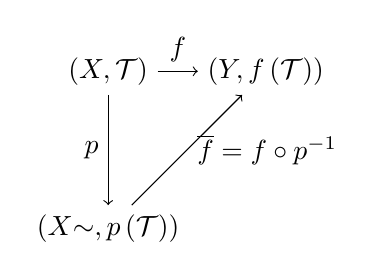
\begin{tikzpicture}[node distance=2cm, auto]
        \node(X) {$\left( X, \mathcal{T} \right)$};
        \node(Y) [right of=X] {$\left( Y, f\left( \mathcal{T} \right) \right)$};
        \node(Z) [below of=X] {$\left( \faktor{X}{\sim}, p\left( \mathcal{T} \right) \right)$};
        \draw[->](X) to node {$f$}(Y);
        \draw[->](X) to node [left] {$p$}(Z);
        \draw[->](Z) to node [right=0.2] {$\overline{f} = f \circ p^{-1}$}(Y);
        \end{tikzpicture}  
        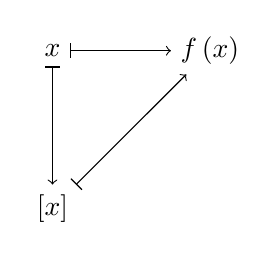
\begin{tikzpicture}[node distance=2cm, auto]
        \node(x) {$x$};
        \node(y) [right of=x] {$f\left( x \right)$};
        \node(z) [below of=x] {$\left[ x \right]$};
        \draw[|->](x) to (y);
        \draw[|->](x) to (z);
        \draw[|->](z) to (y);
        \end{tikzpicture}
        \caption{\textit{Representación de la composición del cociente}}
\end{figure}

\begin{obs}
La relación de equivalencia que vamos a usar es la que viene dada por la relación de \underline{inyectividad} respecto de $f$. Por esta razón, $\overline{f}$ será una biyección.
\end{obs}
\begin{demo}
Sea $z \in Y$ como $f$ es suprayectiva $\exists x \in X: f\left( x \right) = z$. A su vez, $y \in \left[ x \right] \Leftrightarrow f\left( x \right) = f\left( y \right) \Rightarrow \overline{f}\left( \left[ x \right] \right) = z$. Con esto, $\overline{f}$ es sobreyectiva y bien definida.

Sean ahora $\left[ x \right], \left[ y \right] \in \faktor{X}{\sim}$ tal que $\overline{f}\left[ x \right] = \overline{f}\left[ y \right] \Rightarrow f\left( x \right) = f\left( y \right) \Rightarrow \left[ x \right] = \left[ y \right]$. Por tanto, también es inyectiva.
\end{demo}

%TODO: No estoy seguro de como es esta proposición
\begin{prop}
\begin{enumerate}
    \item $\exists \overline{f} \Leftrightarrow x \sim y \Rightarrow f\left( x \right) \sim f\left( y \right)$
    \item $\exists \overline{f} : \overline{f}$ continua $\Leftrightarrow f$ continua.
    \item $\exists \overline{f}: \overline{f} \begin{cases}
        \text{sobre. }\\ 
        \text{iny. 1-1}\\ 
    \end{cases} \Leftrightarrow f \begin{cases}
        \text{sobre.}\\ 
        x \sim y \Leftarrow f \left( x \right) \sim f \left( y \right)
    \end{cases}$

    \item $\overline{f}$ homeomorfa $\Leftrightarrow f$ identificación.
    %TODO: Fix 
    \begin{figure}[H]
        \centering
        \begin{tikzpicture}[node distance=2cm, auto]
        \node(X) {$\left( X, \mathcal{T} \right)$};
        \node(Y) [right=2cm of X] {$\left( Y, \mathcal{T}' \right)$};
        \node(Z) [below=1.5cm of X] {$\left( \faktor{X}{\sim}, \overline{\mathcal{T}} \right)$};
        \draw[->](X) to node {$f$} node [below] {ident.}(Y);
        \draw[->](X) to node [left] {$p$} (Z);
        \draw[->](Z) to node [left=0.2] {$\overline{f}$} node [below=0.3] {homeo.} (Y);
        \end{tikzpicture}  
        \caption{\textit{Relación entre el cociente y una identificación.}}
        \label{fig:relacion_cociente_identificacion}
    \end{figure}
\end{enumerate} 
\end{prop}
\begin{demo}
\begin{enumerate}
    \item Por la definición de $\sim$ y de $\overline{f}$.
    %TODO: Corregir. Creo que se puede usar la propiedad universal
    \item Sea $\overline{f}$ continua. Tomemos $U \in \mathcal{T}' \Rightarrow \overline{f}^{-1}U \in \overline{\mathcal{T}}$. Como $p$ es continua por definición de $\overline{\mathcal{T}}$, $f^{-1} U = p^{-1} \overline{f}^{-1} U \in \mathcal{T}$. Por lo que $f$ es continua.

    Sea ahora $f$ continua. Tomemos $U \in \mathcal{T}' \Rightarrow W = f^{-1}U \in \mathcal{T}$. Al ser $p$ sobreyectiva $W = p^{-1}pW$, es decir, que $pW \in \overline{\mathcal{T}}$ (ya que $p^{-1}\left( p W \right) \in \mathcal{T}$ y la definición de $\overline{\mathcal{T}}$).

    \item (Anterior observación) Si $\overline{f}$ es inyectiva 1-1 $\Rightarrow \underbrace{\overline{f}\left[ x \right] = \overline{f}\left[ y \right]}_{\Leftrightarrow f\left( x \right) \sim f\left( y \right)} \Rightarrow \underbrace{\left[ x \right] = \left[ y \right]}_{\Leftrightarrow x \sim y}$
\end{enumerate}
\end{demo}

\begin{pg}
    Los cocientes son cómodos para definir espacios, las identificaciones son mejores para estudiar las propiedades que tenemos. Conviene pues tener triángulos como el anterior (\ref{fig:relacion_cociente_identificacion}). 

    Se puede contemplar $Y$ como un modelo del cociente. Es decir, utilizamos la identificación como ``modelo teórico'' y el cociente como ``modelo geométrico''. Esto no siempre será posible ya que dependerá de ciertas propiedades geométricas que veremos.
\end{pg}

\begin{ej}[Anteriores]
\begin{itemize}
    \item Circunferencia y el cilindro como cocientes:
    \begin{figure}[H]
        \centering
        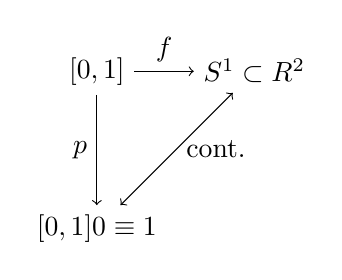
\begin{tikzpicture}[node distance=2cm, auto]
            \node(X) {$\left[ 0, 1 \right]$};
            \node(Y) [right of=X] {$\mathbb{S}^1 \subset \mathbb{R}^2$};
            \node(Z) [below of=X] {$\faktor{\left[ 0, 1 \right]}{0 \equiv 1}$};
            \draw[->](X) to node {$f$} (Y);
            \draw[->](X) to node [left] {$p$} (Z);
            \draw[<->](Z) to node [right] {cont.}(Y);
        \end{tikzpicture}
        %TODO: arreglar distancia X a Y
        \begin{tikzpicture}[node distance=2cm, auto]
            \node(X) {$\left[ 0, 1 \right] \times \left[ 0, 1 \right]$};
            \node(Y) [right=1.5cm of X] {$C \subset \mathbb{R}^3$};
            \node(Z) [below of=X] {$\faktor{\left[ 0, 1 \right] \times \left[ 0, 1 \right]}{\left( 0, t \right) \equiv \left( 1, t \right)}$};
            \draw[->](X) to (Y);
            \draw[->](X) to (Z);
            \draw[<->](Z) to (Y);
        \end{tikzpicture}
        \caption{\textit{En el primero tomamos un segmento de longitud $1$ y ``pegamos'' los extremos, lo que nos da una figura equivalente a un circunferencia. En el segundo, tomamos un rectángulo de área $1$ y ``pegamos'' el lado izquierdo con el derecho directamente.}}
    \end{figure}

    Para la circunferencia tenemos:
    \[
        \faktor{X}{\sim} = \left\{ \left\{ t \right\} : 0 < t < 1, \left\{ 0, 1 \right\} \right\}
    \]
    %TODO: Posiblemente mal
    la biyección entre el cociente y la esfera se da por el punto (3) de la anterior proposición y la continuidad por (2). Por último, la identificación se da por el anterior ejemplo.

    \item Para representar cocientes se utilizan dibujos que indican las identificaciones en los espacios de partida:
    \begin{figure}[H]
        \centering
        \hspace{2cm}
        \begin{tikzpicture}
            \node at (1,2.3) {Cilindro};
            \filldraw[color=cyan, fill=cyan!5, very thick,
                decoration={markings, mark=at position 0.18 with \arrow{>};,
                                      mark=at position 0.59 with \arrow{<};,
                           },
                postaction={decorate}
                ] (0,0) rectangle (2,2);
            \node[cyan] at (0,1.35) {\textbullet};
            \node[cyan] at (2,1.35) {\textbullet};
            \node[gray] at (2.1,1) [right] {$\left( 0, t \right) \equiv \left( 1, t \right)$};
        \end{tikzpicture}
        \begin{tikzpicture}
            \node at (1,2.3) {Banda de Möbius};
            \filldraw[color=cyan, fill=cyan!5, very thick,
                decoration={markings, mark=at position 0.18 with \arrow{>};,
                                      mark=at position 0.67 with \arrow{>};,
                           },
                postaction={decorate}
                ] (0,0) rectangle (2,2);
            \node[cyan](izq) at (0,1.35) {\textbullet};
            \node[cyan](der) at (2,0.67) {\textbullet};
            \node[cyan](O) at (1,1) {\textbullet};
            \draw[-, cyan, dashed] (izq) -- (der);
            \node[gray] at (2.1,1) [right] {$\left( 0, t \right) \equiv \left( 0, 1-t \right)$};
        \end{tikzpicture}
    \end{figure}
\end{itemize}
\end{ej}


\section{Productos finitos}%
\label{sec:productos_finitos_}
El objetivo de esta construcción es, dado un producto cartesiano $Y := X_1 \times \cdots \times X_r$, generar una topología que garantice la continuidad de las aplicaciones $p_i: Y \rightarrow \left( X_i, \mathcal{T}_i \right)$ al ser equipada sobre el mismo, es decir, que haga continuas las proyecciones sobre cada factor. Inmediatamente uno repara en que la discreta sobre $Y$ cumple los requisitos. Sin embargo, el interés está en saber cuál es la topología menos fina que hace las $p_i$ continuas.

Tal y como venimos haciendo en las construcciones anteriores, vamos a tratar de introducir lo mínimo indispensable para verificar la continuidad. En primer lugar, como las preimágenes de abiertos deben ser abiertos, entonces $\forall U_i \in \mathcal{T}_i : p_i^{-1}U_i = X_1 \times \ldots U_i \times \ldots \times X_r $ debe ser un abierto. Como para que pueda ser topología la intersección finita de abiertos tiene que ser abierto, sabemos que $\bigcap_{i=1}^{r} p_i^{-1}U_i = U_1 \times \ldots \times U_r$ debe ser abierto, pero a diferencia de como venía ocurriendo en las construcciones anteriores no podemos decir aún que sea topología porque las uniones arbitrarias no funcionan bien (las uniones de productos no tienen por qué ser producto). 

Sin embargo, se puede demostrar sin demasiada dificultad que el conjunto  $\{U_1 \times \cdots \times U_r \mbox{ donde } U_i \in \mathcal{T}_i\}$ caracteriza una topología en $Y$ de la que es base de abiertos y, de esta manera, ahora sí tenemos determinada de modo único la topología buscada.

\begin{defi}[Topología Producto]
Sea $Y := X_1\times \cdots \times X_n$ un producto cartesiano de espacios topológicos y $p_i : Y \rightarrow (X_i, \mathcal{T}_i)$ las proyecciones sobre cada uno de sus factores, definimos la \textbf{topología producto} como aquella determinada por la base de abiertos:
\[
\mathcal{B} = \left\{ U_1 \times \ldots \times U_r: U_i \in \mathcal{T}_i \right\}
\]
y la denotamos por $\mathcal{T}_1 \times \ldots \times \mathcal{T}_r$.
\end{defi}

\begin{ej}
Si consideramos $\mathcal{T}_u$ en $\mathbb{R}^n$ es automático ver el resultado anterior. Una base de abiertos de la topología son las ``bolas cuadradas'' y estas son productos cartesianos de intervalos de $\mathbb{R}$ con la $\mathcal{T}_u$.
\end{ej}

\begin{theo}[Propiedad universal de la topología producto]
Sea $g: \left( Z, \mathcal{T}'' \right) \rightarrow \left( Y, \mathcal{T}' \right)$ y $p_i: \left( Y, \mathcal{T}' \right) \rightarrow \left( X_i, \mathcal{T}_i \right)$:

    \begin{figure}[H]
        \centering    
            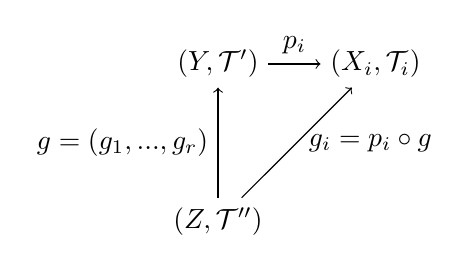
\begin{tikzpicture}[node distance=2cm, auto]
            \node(Y) {$\left( Y, \mathcal{T}' \right)$};
            \node(X) [right of=Y] {$\left( X_i, \mathcal{T}_i \right)$};
            \node(Z) [below of=Y] {$\left( Z, \mathcal{T}'' \right)$};
            \draw[->](Y) to node {$p_i$}(X);
            \draw[->](Z) to node [left] {$g = \left( g_1, ..., g_r \right)$}(Y);
            \draw[->](Z) to node [right=0.2ex] {$g_i = p_i \circ g$}(X);
            \end{tikzpicture}
        \caption{\textit{Ilustración de la composición propuesta}}
        \label{prop_universal_prod_finitos}
    \end{figure}

entonces $\mathcal{T}' = \prod_{i} \mathcal{T}$ si y sólo si
$$
g \text{ cont.} \Leftrightarrow \forall g_i \text{ cont.}
$$
\end{theo}
\begin{demo}
\begin{enumerate}
    \item $\mathcal{T}' = \prod_{i} \mathcal{T}: $ 
    \begin{itemize}
        \item $g$ cont. implica que $g_i$ cont. porque $g_i = p_i \circ g$ y $p_i$ es continua si la topología es la producto.
        \item $g_i$ cont. implica que $g^{-1}\left( U_1 \times \ldots \times U_r \right) = \overbrace{g_1^{-1}\left( U_1 \right)}^{\in \mathcal{T}''} \cap \ldots \cap \overbrace{g_r^{-1}\left( U_i \right)}^{\in \mathcal{T}''} \in \mathcal{T}''$ y como esto es una intersección finita de abiertos, es abierto.
    \end{itemize}

    \item Para demostrarlo, vamos a ver el doble contenido de ambas.
    
    Como la propiedad de caracterización se cumple para cualquier función $g$ que escojamos, podemos elegir la identidad de modo que:
    \begin{figure}[H]
        \centering    
            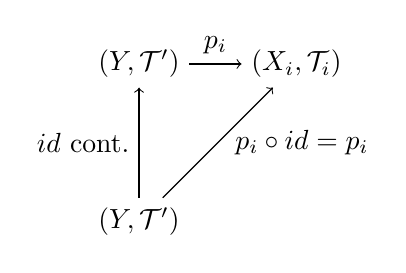
\begin{tikzpicture}[node distance=2cm, auto]
            \node(Y) {$\left( Y, \mathcal{T}' \right)$};
            \node(X) [right of=Y] {$\left( X_i, \mathcal{T}_i \right)$};
            \node(Z) [below of=Y] {$\left( Y, \mathcal{T}' \right)$};
            \draw[->](Y) to node {$p_i$}(X);
            \draw[->](Z) to node [right=0.1cm] {$p_i \circ id = p_i$}(X);
            \draw[->](Z) to node [left] {$id$ cont.}(Y);
            \end{tikzpicture}
    \end{figure}
    la continuidad de $id$ nos asegura la continuidad de $g_i = p_i \circ id = p_i$. Como tenemos que $p_i$ es continua y $\prod \mathcal{T}_i$ es la topología menos fina que verifica esto, entonces $\prod \mathcal{T}_i \subset \mathcal{T}'$.
    
    Para ver el otro contenido, elegimos de nuevo la identidad, pero esta vez la identidad meramente conjuntista:
    \begin{figure}[H]
        \centering    
            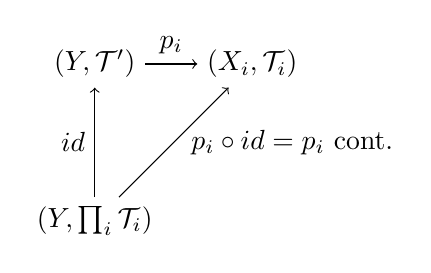
\begin{tikzpicture}[node distance=2cm, auto]
            \node(Y) {$\left( Y, \mathcal{T}' \right)$};
            \node(X) [right of=Y] {$\left( X_i, \mathcal{T}_i \right)$};
            \node(Z) [below of=Y] {$\left( Y, \prod_{i} \mathcal{T}_i \right)$};
            \draw[->](Y) to node {$p_i$}(X);
            \draw[->](Z) to node [right=0.1cm] {$p_i \circ id = p_i$ cont.}(X);
            \draw[->](Z) to node [left] {$id$}(Y);
            \end{tikzpicture}
    \end{figure}
   En este caso, sabemos que $g_i = p_i \circ id = p_i$ es continua porque $p_i$ lo es por construcción. Esto quiere decir que la identidad conjuntista $id$ es continua, es decir, $\forall U \in \mathcal{T}' : id^{-1} U = U \in \prod \mathcal{T}_i$. Por tanto, tenemos que $\mathcal{T}' \subset \prod \mathcal{T}_i$.
\end{enumerate}
\end{demo}

%TODO: Hacer bien
\begin{ej}
La $\mathcal{T}_{\text{rad}}$ no es producto.
\begin{figure}[H]
    \centering
    \begin{tikzpicture}
    \begin{axis}[
        axis lines = middle,
        xlabel = \(\mathcal{T}_1\),
        ylabel = {\(\mathcal{T}_2\)},
        xticklabels={,},
        yticklabels={,},
        xmin=-2,
        xmax=2,
        ymin=-2,
        ymax=2,
    ]
    \addplot [
        domain=0:2, 
        samples=100, 
        color=red,
        dashed,
    ]
    {x^2};
    %\addlegendentry{Eliminamos un ``trozo'' a $\mathbb{R}^2$.}

    \draw[dashed] (0,0) circle (0.5);
    \node(O) at (0,0) {\textbullet};
    \node(U1) at (0,0.3) [left] {\tiny$U_2$};
    \node(U2) at (0.3,0) [below] {\tiny$U_1$};
    \end{axis}
    \end{tikzpicture}
    \caption{\textit{La topología radial no es producto de topologías.}}
\end{figure}

\begin{figure}[H]
    \centering
    \begin{tikzpicture}
    \begin{axis}[
        axis lines = middle,
        xlabel = \(\mathcal{T}_1\),
        ylabel = {\(\mathcal{T}_2\)},
        xticklabels={,},
        yticklabels={,},
        xmin=-1,
        xmax=1.2,
        ymin=-1,
        ymax=1,
    ]
    \addplot [
        domain=0:1, 
        samples=100, 
        color=red,
        dashed,
    ]
    {x^2};
    %\addlegendentry{Eliminamos un ``trozo'' a $\mathbb{R}^2$.}

    \draw[-, dashed] (0,0.49) -- (0.7, 0.49);
    \draw[-, dashed] (0.7,0) -- (0.7, 0.49);
    \node(O) at (0,0) {\textbullet};

    \node at (0,0.49)  {\tiny \textbullet};
    \node(U1) at (0,0.35) [left] {\tiny$y_1 \not\in U_1$};

    \node at (0.7,0)  {\tiny \textbullet};
    \node(U2) at (0.6,0) [below] {\tiny$U_1 \ni x_1$};
    \node at (0.7,0.49)  {\tiny \textbullet};
    \node(xy) at (0.7,0.49) [right] {\tiny$\left( x, y \right) \not\in U$};
    \end{axis}
    \end{tikzpicture}
    \caption{\textit{La topología radial no es producto de topologías.}}
\end{figure}

\begin{figure}[H]
    \centering
    \begin{tikzpicture}
    \begin{axis}[
        axis lines* = middle,
        height=2cm,
        width=5cm,
        scale only axis=true,
        ytick=\empty,
        xtick=\empty,
        xmin=-0.2,
        xmax=1,
        ymin=-0.3,
        ymax=0.6,
    ]
    \node(O) at (0,0) {\textbullet};

    \draw[<->] (0,0.3) -- (0.6,0.3);
    \node at (0.3,0.3) [above] {$\varepsilon$};

    \draw[<->] (0,-0.1) -- (0.6,-0.1);
    \node at (0.3,-0.1) [below] {\tiny No hay};

    \node at (0.6,0) {\tiny$\mid$};
    \node at (0.8,0) {\tiny$\mid$};
    \node at (0.8,0) [below] {\tiny$x_1$};
    \node at (0.9,0) {\tiny$\mid$};
    \node at (0.9,0) [below] {\tiny$x_2$};
    \node at (1.0,0) {\tiny$\mid$};
    \end{axis}
    \end{tikzpicture}
    \caption{\textit{La topología radial no es producto de topologías.}}
\end{figure}
\begin{demo}
    Tomamos un abierto y veamos que no es producto. 
    %TODO: Dibujo

    Supongamos que sí:
    $U = \mathbb{R}^2 \setminus $ arco $\ni \left( 0, 0 \right) \Rightarrow U_1 \times U_2 \subset U$ y $\left( 0, 0 \right) \in U_1 \times U_2 \subset \mathcal{T}_{\text{rad}}$. Tomando $x_1 \in U_1$ y vemos $x = x_1 \cap r$ con $r$ línea vertical por $x_1$ con esto $y_1 = x \cap l$ con $l$ línea horizontal por $x$ no pertenece a $U$ (de lo contrario el producto $y_1$ con $x_1 = x$ pertenecería). Por tanto, $I_k = \left[ \left( 0, y_k \right), \left( x_k, y_k \right) \right]$ no tiene ningún punto en $U_1 \times U_2$. Haciendo converger $I_k$ hacía $0$ para cualquier recta por $0$ tendremos un $I_k$ que tenga intersección con la recta, es decir, la recta tendrá un punto que no pertenezca al abierto y $U$ no sería abierto ¡!

    Con esto, $\nexists x_k \rightarrow 0 \Rightarrow$ habrá un intervalo $\left( 0, \varepsilon \right)$ en el eje $x$ que no pertenece a $U_1$ y tendremos un ``vacío'' que de nuevo incumple que $U$ es abierto.
\end{demo}
\end{ej}

\begin{prop}
\begin{enumerate}
    \item Las proyecciones $p_i: Y \rightarrow X_i$ sobre los factores del producto son aplicaciones abiertas. 
    \item La aplicación natural\footnote{Obviamente, con los $a_i$ fijados.} que sumerge un factor en el producto 
	\begin{align*}
	 \alpha_j : X_j &\longrightarrow Y \\
	 x_j &\longmapsto \left( a_1, \ldots, x_j, \ldots, a_r \right)	
	\end{align*}	    
     es una inmersión que llamamos aplicación parcial.
\end{enumerate}
\end{prop}
\begin{demo}
\begin{enumerate}
    \item Nos vale con probarlo para una base: $p_i\left( U_1 \times \ldots \times U_r \right) = U_i$ 
    \item Trivialmente es inyectiva y continua. Por último, $X_i \rightarrow j\left( X_i \right)$ es homeomorfismo, es decir, es abierta porque:
    \[
    \begin{cases}
        \alpha_j\left( X_j \right) = \{a_1\} \times \ldots \times X_j \times \ldots \times \{a_r\} \\
        \alpha_j\left( U_j \right) = \{a_1\} \times \ldots \times U_j \times \ldots \times \{a_r\} = \alpha_j\left( X_j \right) \cap \left( X_1 \times \ldots \times U_j \times \ldots \times X_r \right) 
    \end{cases}
    \]
    que es abierto porque estamos restringiendo la topología producto a $\left\{ a_1 \right\} \times \ldots \times X_i \times \ldots \times \left\{ a_r \right\} = \alpha_j\left( X_j \right)$.
\end{enumerate}
\end{demo}

\begin{ej}
El ejemplo ahora de $\mathcal{T}_{\text{rad}}$ simplemente es porque si fuese producto sus elementos deberían ser la usual y el producto de usuales es usual que es distinta de la radial.
\end{ej}

\begin{pg}
En una topología producto todo ``se genera en productos''.
\begin{ej}
\begin{itemize}
    \item Bases de entornos: $\mathcal{V}^a = \mathcal{V}^{a_1} \times \ldots \times \mathcal{V}^{a_r} \stackrel{mut??}{=} \{V_1 \times \ldots \times V_r: V_i \in \mathcal{V}^{a_i}\} \left( a \in Y \right)$.
    \item Base de abiertos: $\mathcal{B} = \mathcal{B}_1 \times \ldots \times \mathcal{B}_r = \{B_1 \times \ldots \times B_r: B_i \in \mathcal{B}_i\}$ (esto repite la construcción de $\prod_{i} \mathcal{T}_i$)
\end{itemize}
\end{ej}
\end{pg}


%TODO: Cambiar e_i por j_i?
\section{Sumas (finitas)}%
\label{sec:sumas_finitas}
Supongamos que tenemos $e_i: \left( X_i, \mathcal{T}_i \right) \rightarrow Y = X_1 + \ldots + X_r = \left( X_1 \times \left\{ 1 \right\} \right) \cup \ldots \cup \left( X_r \times \left\{ r \right\} \right), 1 \le i \le r: x_i \mapsto \left( x_i, i \right)$ (ponemos los índices para hacerlos disjuntos) y buscamos hacerlas continuas. Trivialmente, podemos hacer que la topología en $Y$ sea la trivial, sin embargo, esto carece de interés. Por esta razón, buscamos la topología \underline{más fina} que haga $f$ continua.

Debido a que, $\forall U_i \in \mathcal{T}_i,\ e_i^{-1}\left( U_i \times \left\{ i \right\} \right)$ debe ser abierto, podemos definir lo siguiente:
\begin{defi}
Llamamos \textbf{topología suma}, $\sum_{i=1}^{k} \mathcal{T}_i$, a aquella que viene determinada por la siguiente base:
\[
\mathcal{B} = \left\{ U_1 \times \left\{ 1 \right\}, \ldots, U_r \times \left\{ r \right\}: U_i \in \mathcal{T}_i, 1 \le i \le r \right\}
\]
\end{defi}

\begin{obs}
Tenemos que los $\left\{ i \right\} \times X_i \in \sum_{i=1}^{r} \mathcal{T}_i$ son sumandos abiertos y cerrados (porque el complementario es la intersección del resto de sumandos que son abiertos?).
\end{obs}

\begin{prop}
Con la anterior definición sabemos que 
\[
e_i: \left( X_i, \mathcal{T}_i \right) \rightarrow \left( X_i\times \{i\}, \mathcal{T}|_{X_i \times \{i\}} \right),\ \forall i \in \left\{ 1, \ldots, r \right\}
\]
es inmersión abierta y cerrada.
\end{prop}
\begin{demo}
\begin{itemize}
    \item Inmersión abierta: $e_i\left( U_i \right) = U_i \times \{i\} \in \mathcal{T}$
    \item Cerrada: $Y\setminus e_i\left( X_i \right) = Y \setminus X_i \times \{i\} = \bigcup_{j \neq i} X_j \times \{j\} \in \mathcal{T}$
\end{itemize}
\end{demo}

%TODO: Fix teorema
\begin{theo}[Caracterización topología suma]
Sea $g: \left( Y, \mathcal{T}' \right) \rightarrow \left( Z, \mathcal{T}'' \right)$ y $e_i: \left( X_i, \mathcal{T}_i \right) \rightarrow \left( Y, \mathcal{T}' \right)$. Entonces:
    \[
    \mathcal{T}' = \mathcal{T}_1 + \ldots + \mathcal{T}_r \Leftrightarrow  
    \]
    \begin{equation}\label{eq:prop_universal_sum}
        \forall g \left[ g \text{ cont.} \Leftrightarrow \forall g_i \text{ cont.} \right]
    \end{equation}

    \begin{figure}[H]
        \centering    
            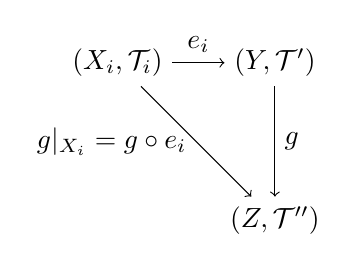
\begin{tikzpicture}[node distance=2cm, auto]
            \node(X) {$\left( X_i, \mathcal{T}_i \right)$};
            \node(Y) [right of=X] {$\left( Y, \mathcal{T}' \right)$};
            \node(Z) [below of=Y] {$\left( Z, \mathcal{T}'' \right)$};
            \draw[->](X) to node {$e_i$}(Y);
            \draw[->](X) to node [left] {$g|_{X_i} = g \circ e_i$}(Z);
            \draw[->](Y) to node {$g$}(Z);
            \end{tikzpicture}
        \caption{\textit{Ilustración de la composición propuesta}}
        \label{prop_universal_sum_finitas}
    \end{figure}
\end{theo}
%TODO: Tal vez hacerlo bien?
\begin{demo}
    Análoga a las anteriores construcciones.
\end{demo}

\begin{pg}
Localmente $Y = X_1 + \ldots + X_r$ es como sea cada $X_i$. Por ejemplo, las bases de entornos de $Y$ son las de los sumandos. Globalmente, se trata cada sumando separadamente. Por ejemplo, las bases de abiertos de los sumandos se unen para dar una base de abiertos de $Y$. Olvidando el tecnicismo $X_i \times \{i\} \equiv X_i$:
\begin{center}
   $Y$ es unión disjunta de los sumandos\\
   Los sumando son subespacios abiertos y cerrados de $Y$
\end{center}
Es un formalismo para hacer cómodamente otras construcciones. Por ejemplo, ``pegar dos discos por sus bordes'' sería:
\begin{gather*}
    \text{Disco } D \subset \mathbb{R}^2: x^2 + y^2 \le 1, \text{ borde } \partial D = \mathbb{S}^1: x^2 + y^2 = 1\\
    %TODO: Fix cociente
    \faktor{D_1 + D_2}{\sim} \quad \overbrace{\left( p, 1 \right)}^{\in \partial D} \sim \left( p, 2 \right) 
.\end{gather*}

\begin{figure}[H]
    \centering
    \incfig{dos-discos.}
    \caption{\textit{Dos discos}}
    \label{fig:dos-discos.}
\end{figure}
y más elaborado $h: \partial D \stackrel{\text{homeo.}}{\approx} \partial D$ con $\overbrace{p}^{\in \partial D} \sim h\left( p \right)$.

Finalmente, hay otros conceptos de ``suma'' más significativos que veremos en algún ejemplo.
\end{pg}


\section{Espacios proyectivos reales}%
\label{sec:espacios_proyectivos_reales}
\subsection{Geometría lineal}
\label{sub:geometría_lineal}
En primer lugar, veamos un repaso de lo visto en geometría lineal sobre espacios proyectivos.
\begin{defi}[Espacio proyectivo real]    
Usando $\sim$, proporcionalidad: 
\[
\mathbb{R}P^n = \mathbb{P}^{n} = \faktor{\mathbb{R}^{n+1}\setminus \{0\}}{\sim} \Rightarrow \mathbb{P}^{n} = \{\text{rectas vectoriales de } \mathbb{R}^{n+1}\}     
\]
Que en coordenadas es:
\begin{align*}
    \pi: \mathbb{R}^{n+1} \setminus \{0\} &\rightarrow \mathbb{P}^{n}\\
    \left( x_0, \ldots, x_n \right) &\mapsto \left( x_0 : \ldots : x_n \right) 
.\end{align*}
\end{defi}
\begin{obs}
Las ecuaciones serán de la forma: $h\in \mathbb{R}\left[ x_0, \ldots, x_n \right]$ homogénea $\Rightarrow \begin{cases}
    h\left( x \right) = 0\\
    h\left( x \right) \neq 0
\end{cases}$ está bien definido en $\mathbb{P}^{n}$.
Sabemos que el grado de la ecuación homogénea $h$ nos dará lugar a:
\begin{itemize}
    \item Grado \underline{1}: Variedades proyectivas lineales.
    \item Grado \underline{2}: Cuádricas proyectivas.
    \item Grado \underline{arbitrario}: Variedades proyectivas algebraicas.
\end{itemize}
\end{obs}

\begin{defi}[Cartas afines]
Sea $H \subset \mathbb{P}^n$ un hiperplano proyectivo. Entonces, tenemos un hiperplano lineal $\hat{H} \subset \mathbb{R}^{n+1}$, con una forma lineal asociada $h = 0$, de la siguiente forma:
\[
H = \faktor{\hat{H}\setminus \left\{ 0 \right\}}{\sim}
\]
Decimos que $H$ es \textbf{hiperplano del infinito} de la \textbf{carta afín} $U = \mathbb{P}^n \setminus H$.
\end{defi}
\begin{prop}
La aplicación 
\[
\pi|: \underbrace{\left\{ h = 1 \right\}\subset \mathbb{R}^{n+1} \setminus \left\{ 0 \right\}}_{\text{Hiperplano afín}} \rightarrow \underbrace{\mathbb{P}^{n} \setminus H}_{\left\{ h \neq 0 \right\}} = U
\]
es una biyección.
\end{prop}

\subsection{Topología de espacio proyectivos}
\label{sub:topología_de_espacio_proyectivos}
Para la topología en $U$ usaremos la imagen directa de la usual en $\left\{ h = 1 \right\} \subset \mathbb{R}^{n+1}$
\begin{prop}
Con la anterior suposición tenemos que la aplicación:
\[
\pi|: \{h = 1\} \rightarrow U
\]
es un \underline{homeomorfismo}.     
\end{prop}
\begin{demo}
Ya sabemos que es biyección por lo que queda ver que es continua y abierta/cerrada. Continua lo será por tener $U$ la topología imagen directa. Y abierta porque???%TODO
\end{demo}
%TODO: Creo que esta demostración no es de esto.
%\begin{demo}
%Veamos lo que tenemos:
%\begin{figure}[H]
%    \centering
%        \begin{tikzpicture}[node distance=2cm, auto]
%        \node(X) {$\mathbb{R}^{n+1} \setminus \left\{ 0 \right\}$ usual};
%        \node(Z) [below of=X] {$U \subset \mathbb{P}^n$ cociente};
%        \node(Y) [left=1.2cm of Z] {$\mathbb{R}^{n+1} \supset \left\{ h = 1 \right\}$};
%        \draw[->](X) to node [left] {$\pi$}(Z);
%        \draw[->](Y) to node [below] {homeo.}(Z);
%        \end{tikzpicture}
%    \captionsetup{font={color=gray}}
%    \caption[gray]{\textit{Composición propuesta}}
%    \label{}
%\end{figure}
%Tomemos $W \subset U \begin{cases}
%    \text{cociente: } \pi^{-1} \left( W \right) \ab \mathbb{R}^{n+1} \setminus \left\{ 0 \right\}\\
%    \text{homeo: } \pi^{-1}\left( W \right) \cap \left\{ h = 1 \right\} \ab \left\{ h=1 \right\}
%\end{cases}$.    
%Cociente $\Rightarrow$ homeomorfismo es trivial y significa que $\pi|_{\left\{ h=1 \right\}}$ es continua. Homeomorfismo $\Rightarrow$ cociente porque:
%\[
%\pi^{-1}\left( W \right) = \text{cono de } \underbrace{\pi^{-1}\left( W \right) \cap \left\{ h = 1 \right\}}_{A}
%\]
%Como $\left\{ h=1 \right\} \supset A$ abierto $\Leftrightarrow \text{cono}\left( A \right) \ab \mathbb{R}^{n+1} \setminus \left\{ 0 \right\}$ donde cono$\left( A \right) = \left\{ \lambda a: a \in A, \lambda \in \mathbb{R} \setminus \left\{ 0 \right\} \right\}$
%\end{demo}

\begin{prop}
La siguiente definición es topología en $\mathbb{P}^n$:
\[
W \text{ abierto si } W \cap U \text{ es abierto } \forall U \text{ carta afín.}
\]
\end{prop}
\begin{demo}
%TODO
Ni idea
\end{demo}

%TODO: Fix topologia
\begin{prop}[Topología en Pn]    
\begin{itemize}
    \item \underline{Cociente} de la usual vía $\mathbb{R}^{n+1}\setminus \{0\} \xrightarrow{\pi} \mathbb{P}^{n}: \left( x_0, \ldots, x_n \right) \mapsto \left( x_0 : \ldots : x_n \right)$
    \item ``\underline{Suma}'' de las definidas en las cartas afines:
    \[
        W \text{ abierto si } W \cap U \text{ es abierto } \forall U \text{ carta afín.} 
    \]
\end{itemize}
Estas dos topologías coinciden.
\end{prop}
\begin{demo}
\begin{enumerate}
    \item $U$ es abierto en la topología cociente ya que $\pi^{-1} U = \{h \neq 0\}$ es abierto usual.
    \item La topología cociente en $U$ coincide con la topología de carta afín:
    %¡¡¡¡IMPORTANTE!!!!: TOCAR LO MINIMO POSIBLE
    \begin{figure}[H]
        \centering
        \begin{tikzpicture}
            \node(top) at (0,0) {$W \subset U : \pi^{-1}W = $ cono sobre $\underbrace{\left( \pi^{-1} W \right)\cap \left\{ h = 1 \right\}}_{= \left( \pi|_{\left\{ h=1 \right\}} \right)^{-1}W}$}; 
            %Izquierda
            \draw[->] (-2.4,0) -- (-2,0.1);
            \node at (-2,0) [below, text width=2cm] {para la top. cociente};
            %Derecha
            \draw[->] (4.4,-0.3) -- (3.5,-0.3);
            \node at (5.5,0.2) [below, text width=2cm] {para la top. de carta afín};

            \draw[-{implies},double] (0,0) -- (0,-2);

            \node(bottom) at (0.7,-2.2) {$\pi^{-1}W \ab \mathbb{R}^{n+1} \Leftrightarrow \left( \pi|_{\left\{ h=1 \right\}}^{-1} \right)W \ab\left\{ h=1 \right\}$};

            %Izquieda
            \draw[implies-implies,double] (-1.35,-2.4) -- (-1.35,-3);
            \node at (-1.35,-3) [below, text width=2cm] {$W$ abierto top. cociente};
            %Derecha
            \draw[implies-implies,double] (2.55,-2.4) -- (2.55,-3);
            \node at (2.55,-3) [below, text width=2cm] {$W$ abierto top. carta afín};
        \end{tikzpicture}
        \captionsetup{font={color=gray}}
        \caption[gray]{\textit{Equivalencia entre las topologías cociente y suma.}}
        \label{fig:cociente_suma_equivalentes}
    \end{figure}
    \item[1. + 2.] $\Rightarrow $ La top. cociente está generada por las topologías de las cartas afines, que forman un recubrimiento abierto de $\mathbb{P}^{n}$.
\end{enumerate}
\end{demo}

%TODO: Fix orden
\begin{prop}
    En este caso, la $\mathcal{T}_{\text{cociente}}$ tendrá como base: $\left\{ \pi\left( B \right) \subset U : B \ab \left\{ h = 1 \right\},\ h \in \mathbb{P}\left[ x_0, \ldots, x_n \right] \right\}$ homogéneo de grado $1: G = \bigcup_{U} G \cap U$ abierto en $\mathbb{P}^n$ y abierto en $U$.
\end{prop}

\begin{obs}
    En $U_1 \cap U_2$ la topología definida por $\pi_1 = $ definida por $\pi_2$.
\end{obs}

\begin{obs}
De lo anterior deducimos:
\begin{enumerate}
    \item $U_1, U_2$ dos cartas afines $\Rightarrow U_1 \cap U_2$ abiertos.
    \begin{demo}
    \[
        \text{Cartas afines: } U_i = \{h_1 \neq 0\} \begin{cases}
                \pi|: \{h_1 = 1\} \rightarrow U_1 \text{homeo.}\\
                \left( \pi_1 \right)^{-1}\left( U_1 \cap U_2 \right) = \{h_1 = 1, h_2 \neq 0\} \ab \{h_1 = 1\}  
        \end{cases}  
    \]
    \end{demo}
    \item Las topologías de $U_1$ y $U_2$ coinciden en $U_1 \cap U_2$.
    \begin{demo}
        De nuevo conviene entenderlo con cartas:
        \begin{figure}[H]
            \centering
                \begin{tikzpicture}[node distance=2cm, auto]
                %Lado izquierdo
                \node(X) {$\mathbb{R}^{n+1} \supset \left\{ h_1=1, h_2 \neq 0 \right\}$};
                \node(Y) [below=1cm of X] {$\mathbb{R}^{n+1} \supset \left\{ h_1 \neq 0, h_2=1 \right\}$};
                \draw[<->] (X) to node [left] {\footnotesize homeo?} (Y);
                \node(Z) [below right=0.3cm and 1.2cm of X] {$U_1 \cap U_2$};
                \draw[->] (X) to node [text width=1.1cm, font=\tiny\linespread{0.8}\selectfont] {homeo. para $U_1$} (Z);
                \draw[->] (Y) to node [pos=0.8, below=0.15, text width=1.1cm, font=\tiny\linespread{0.8}\selectfont] {homeo. para $U_2$} (Z);
                %Lado derecho
                \draw [decorate,
                    decoration = {brace}] (4.7,-0.2) --  (4.7,-1.6);
                \draw[-implies,double] (5,-0.9) -- (6,-0.9);
                \node(x) at (7.5,-0.2) {$x = \faktor{y}{h_1\left( y \right)}$};
                \node(y) [below=0.6cm of x] {$y = \faktor{x}{h_2\left( x \right)}$};
                \draw[<->] (x) to node [right=1cm] {\footnotesize homeos usuales} (y);
                \end{tikzpicture}
            %TODO: Ni idea de que significa esto
            %\caption{}
            %\label{}
        \end{figure}
    \end{demo}
\end{enumerate}
\end{obs}

%TODO: Esto es posible que se pueda agrupar mejor (hasta Möbius)
\begin{defi}[Atlas afín canónico]
No se suelen utilizar todas las cartas afines: $n + 1$ distintas ya cubren $\mathbb{P}^{n}$. Típicamente $\mathbb{P}^{n} = U_0 \cup \ldots \cup U_n$ con:
\[
    U_i = \{x_i \neq 0\} \leftrightarrow \{\underbrace{x_i = 1}_{\equiv \mathbb{R}^n}\}: \left( x_0 : \ldots : x_i : \ldots : x_n \right) \mapsto \left( \frac{x_0}{x_i}, \ldots, \underbrace{\not1}_{\mathbb{R}^n \rightarrow}, \ldots, \frac{x_n}{x_i} \right), 0 \le i \le n
\]
\end{defi}

\begin{prop}[Cociente antipodal]
    Toda recta de $\mathbb{R}^{n + 1}$ corta a $\mathbb{S}^{n}: x_0^2 + \ldots + x_n^2 = 1$ en dos puntos \underline{antipodales}, así que denotamos un ``sub'' cociente, que es también identificación.
    \begin{figure}[H]
        \tikzset{
            draw=none,
            subset/.style={
                edge node={node [sloped, allow upside down, auto=false]{$\subseteq$}}
            }
        }
        \centering
            \begin{tikzpicture}[node distance=2cm, auto]
            \node(X) {$\mathbb{R}^{n+1}\setminus \left\{ 0 \right\}$};
            \node(Y) [right=0.2cm of X] {$\mathbb{S}^n$};
            \node(Z) [below of=X] {$\mathbb{R}^n$};
            \node at (1.03,-0.01) {$\supset$};
            \draw[->](X) to (Z);
            \draw[->](Y) to node [right] {$\pi|$} (Z);
            \end{tikzpicture}
        \caption{\textit{Cociente antipodal de $\mathbb{S}^n$}}
        \label{fig:cociente_antipodal_Sn}
    \end{figure}
\end{prop}
\begin{demo} 
    Como antes tenemos conos: $\pi^{-1}W = $ cono sobre $\underbrace{\mathbb{S}^n \cap \pi^{-1}W}_{= \left( \pi / \mathbb{S}^n \right)^{-1} W}$.
\end{demo}
\begin{obs}
    Las cartas afines tienen una representación muy conveniente:
    %TODO: Fix imagen
    \begin{center}
        \includegraphics[scale=0.3]{images/repr_carta_afin} 
    \end{center}
\end{obs}

%TODO: Demostrar que un hemisferio tiene una identificación al proyectivo. 
\begin{prop}[Cociente de un disco]
Consideremos un disco:
\[
    E = \{h = 0, x_0^2 + \cdots + x_n^2 = 1\} = \partial \begin{cases}
        \overline{S}_+ = \mathbb{S}^n \cap \{h \ge 0\} \text{ hemisferio cerrado.} \\
        D^n = \{h = 0, x_0^2 + \cdots + x_n^2 \le 1\} \text{ disco.} 
    \end{cases} 
\]
\begin{figure}[H]
    \centering
        \begin{tikzpicture}[node distance=2cm, auto]
        \node(X) {$\overline{S}_+$};
        \node(Y) [right of=X] {$D^n$};
        \node(Z) [below of=X] {$\mathbb{R}^n$};
        \draw[->](X) to node {$\alpha$}(Y);
        \draw[->](X) to node [left] {$\pi$}(Z);
        \draw[->](Y) to node {$\pi \circ \alpha^{-1}$}(Z);
        \node(E1) [above=0.4 of X] {E};
        \node(S1) at (-0.15,0.5) [rotate=90] {$\stackrel{\partial}{\subset}$};
        \node(E2) [above=0.4 of Y] {E};
        \node(S2) at (2.15,0.5) [rotate=90] {$\stackrel[\partial]{}{\subset}$};
        \draw[-, double] (0.5, 0.9) -- (1.5, 0.9);
        \end{tikzpicture}
    \incfig[0.4]{proyectivo_disco}
    \caption{\textit{$\mathbb{R}^n$ se obtiene identificando puntos antipodales del borde de un disco.}} 
    \label{fig:proyectivo_disco}
\end{figure}
\end{prop}

\begin{ej}
$\mathbb{P}^{2} \setminus D^2 = $ banda de Möbius.
%TODO: Fix imagen
\begin{center}
    \includegraphics[scale=0.3]{images/banda_moebius} 
\end{center}
\end{ej}


\chapter{Separación}%
\label{cha:separacion}

\section{Concepto}%
\label{sec:concepto}
\begin{defi}
Un espacio $X$ es \textbf{Hausdorff} o $T_2$ si para cada par de puntos distintos $x, y \in X$ existen entornos disjuntos:
\[
\forall x, y \in X,\ \exists V^x, V^y: V^x \cap V^y = \emptyset
\]
\end{defi}
Hay otras formas de separación, más débiles o más fuertes, pero nos contentaremos con ésta al ser la más intuitiva.

\begin{obs}
\begin{enumerate}
    \item Si existen entornos disjuntos, existen entornos abiertos disjuntos.
    \begin{demo}
        $\forall V^{\text{ent.}},\ \exists U^{\text{ent. ab.}}: V \supset U$
    \end{demo}
    \item Si $X$ es Hausdorff, los puntos son cerrados.
    \begin{demo}    
    Sea $x \in X$
    \[
    \forall y \in X \setminus \left\{ x \right\},\ \exists U^y \not\ni x \Rightarrow X \setminus \{x\} = \bigcup_{y \neq x} U^y  \text{ es abierto.} 
    \]
    También lo podemos ver como entorno de todos sus puntos.
    \end{demo}
    \item $\left( X, \mathcal{T}_{\text{CF}} \right)$ no es Hausdorff. Sin embargo, tiene puntos cerrados.
    \begin{demo}
        No es Hausdorff porque, si $X$ es infinito, dos abiertos cualesquiera se cortan.
        Sean $U_1, U_2 \in \mathcal{T}_{\text{CF}} \Rightarrow X \setminus U_1, X \setminus U_2$ son finitos y como $X$ es infinito $\Rightarrow \exists x \not\in X \setminus U_1 \cup X \setminus U_2 \Rightarrow x \in U_1 \cap U_2$.
    \end{demo}

    \item $\left( \mathbb{R}^n, \mathcal{T}_{u} \right)$ es Hausdorff. Como $\mathcal{T}_{u} \subset \mathcal{T}_{\text{rad}}$, esta última también es Hausdorff.
    \begin{demo}    
    Sean $x \neq y \Rightarrow B\left( x, \varepsilon \right) \cap B\left( y, \varepsilon \right) = \emptyset$ si $\varepsilon < \frac{\lVert x - y \rVert}{2}$.
    \end{demo}

    \item En $\left( X, \mathcal{T}_a \right)$ el punto $a$ no es cerrado. Por lo tanto no es Hausdorff. 
    \begin{demo}
    Veamos que $a$ no es cerrado: $a \not\in X \setminus \{a\} \Rightarrow X \setminus \{a\}$ no es abierto: $\forall x \neq a, U^x \supset \{a, x\} \ni a$.   
    \end{demo}
\end{enumerate}
\end{obs}

\begin{prop}
Sean $f, g: X \rightarrow Y$ continuas con $Y$ Hausdorff $\Rightarrow \{f = g\} = \{x \in X : f\left( x \right) = g\left( x \right)\}$ es cerrado.
\end{prop}
\begin{demo}
En primer lugar, veamos que si un punto cumple $f\left( x \right) \neq g\left( x \right) \Rightarrow$ tiene un entorno cuyos puntos cumplen todos que $f\left( y \right) \neq g\left( y \right)$. Con esto, tendremos que $\left\{ f \neq g \right\}$ es entorno de todos sus puntos y, por tanto, abierto.
\begin{enumerate}
    \item $f\left( x \right) \neq g\left( x \right) \xRightarrow{T_2} \exists V^{f\left( x \right)} \cap V^{g\left( x \right)} \stackrel{*}{=} \emptyset \xRightarrow{\text{cont.}} f^{-1}V^{f\left( x \right)} \cap g^{-1}V^{g\left( x \right)} = W^x$ entorno de $x$ (cada uno es entorno de $x$ y no son vacíos porque $x$ pertenece a ellos).

    \item Vemos que $W^x \cap \{f = g\} = \emptyset: y \in V^x \Rightarrow \begin{cases}
        f\left( y \right) \in V^{f\left( x \right)} \\
        g\left( y \right) \in V^{g\left( x \right)} 
    \end{cases} \xRightarrow{*} f\left( y \right) \neq g\left( y \right)$

    \item[1. + 2.] $X\setminus \{f = g\} = \{f \neq g\}$ es entorno de todos sus puntos, luego abierto, es decir, $\{f = g\}$ es cerrado.
\end{enumerate}
\end{demo}

\begin{coro}
Si $\left\{ f = g \right\}$ es un subconjunto denso, es decir, $\exists A \subset X: \overline{A} = X$ y $\left\{ f = g \right\}_A$, entonces $f \equiv g$.
\end{coro}
\begin{demo}
$f|_A = g|_A \Rightarrow \{f = g\} \supset A \xRightarrow{\text{prop.}} \overline{\left\{ f = g \right\}} = \{f = g\} \supset \overline{A} = X \Rightarrow \boxed{X = \left\{ f = g \right\}}$.
\end{demo}

\begin{obs}
Este último resultado nos permite extender de forma única una función continua $f$ a su adherencia.
\end{obs}

\begin{ej}[Importante]
Un caso importante en el que $Y$ es Hausdorff es: 
\[
f: X \rightarrow Y = \mathbb{R}
\]
\end{ej}

\begin{obs}
$f: X \rightarrow Y$ continua con $Y$ Hausdorff $\Rightarrow f^{-1}\left( y \right)$ cerrado $\forall y \in Y$.
\begin{demo}
Porque los puntos de $Y$ son cerrados y la preimagen de cerrados por continuidad es cerrada.
\end{demo}
\end{obs}

\section{Tabla de comportamiento}%
\label{sec:tabla_de_comportamiento}
Se trata de saber si la propiedad se conserva por las construcciones que hemos visto.

Se tiene que:
\begin{table}[H]
\centering
\begin{tabular}{| c | c | c | c | c |}
    \hline
    & Subespacios & Cocientes & Productos & Sumas\\
    \hline
    $T_2$ & $\Rightarrow$ & \ding{55} & $\Leftrightarrow$ & $\Leftrightarrow$\\
    \hline
\end{tabular}
\caption{\textit{Tabla que nos indica como se conserva la propiedad Hausdorff en distintas construcciones. Las sumas y los productos son finitos.}}
\end{table}
\begin{demo}
\begin{enumerate}
    \item\label{it:subespacio_hausdorff} Veamos como los subespacios conservan la propiedad: 

    Sea $Y \subset X = T_2: y_1, y_2 \in Y \Rightarrow \exists \underbrace{V^{y_1}}_{\text{En } X}  \cap \underbrace{V^{y_2}}_{\text{En } X} = \emptyset \Rightarrow \underbrace{\left( V^{y_1} \cap Y \right)}_{\text{En } Y}  \cap \underbrace{\left( V^{y_2} \cap Y \right)}_{\text{En } Y} = \emptyset$.

    \item Veamos un contraejemplo de un cociente que no conserva Hausdorff: 

    Sea $Y = \faktor{\mathbb{R}}{\mathbb{Q}}: \begin{rcases}
        y_1 = \mathbb{Q} \in Y\\
        y_2 = \sqrt{2} \in Y
    \end{rcases} \nexists V^{y_1} \cap V^{y_2} = \emptyset: $ todo entorno abierto de $\sqrt{2}$ contiene racionales, luego al saturar, contiene $\mathbb{Q}$. Con esto, todo abierto en el cociente (recordemos que en el cociente los abiertos son imágenes por proyección de los saturados) contiene este punto y, por tanto, la intersección nunca es disjunta.

    \item Veamos que el producto conserva la propiedad: 

    $X$ y $Y$ son ambos $T_2 \Leftrightarrow X \times Y$ Hausdorff.
    \begin{itemize}
        \item[$\Rightarrow)$] Tomamos $\left( x_1, y_1 \right) \neq \left( x_2, y_2 \right) \in X \times Y$. Esto es posible en dos casos:
        \begin{itemize}
            \item $x_1 \neq x_2$. Como $X$ es $T_2 \Rightarrow \exists V^{x_1} \cap V^{x_2} = \emptyset \Rightarrow \left( V^{x_1} \times Y \right) \cap \left( V^{x_2} \times Y \right) = \emptyset$ 
            \item $y_1 \neq y_2$ podemos hacer lo mismo porque $Y$ es también $T_2$.
        \end{itemize}

    %TODO: Corregir caption 
    \begin{figure}[H]
        \centering
        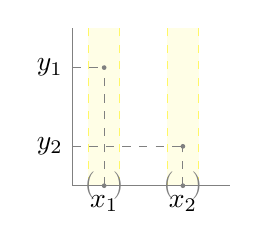
\begin{tikzpicture}
            \draw[-, gray] (0,0) -- (0,2);

            %Rectangulo izq
            \fill[fill=yellow!10, very thick, dashed] (0.2,2) rectangle (0.6,0);
            \draw[-, yellow!60] (0.2,0) -- (0.6,0);
            \draw[-, yellow!60, dashed] (0.2,0) -- (0.2,2);
            \draw[-, yellow!60, dashed] (0.6,0) -- (0.6,2);
            \fill[gray] (0.4,0) circle (0.03);

            %Rectangulo der
            \fill[fill=yellow!10, very thick, dashed] (1.2,2) rectangle (1.6,0);
            \draw[-, yellow!60] (1.2,0) -- (1.6,0);
            \draw[-, yellow!60, dashed] (1.2,0) -- (1.2,2);
            \draw[-, yellow!60, dashed] (1.6,0) -- (1.6,2);
            \fill[gray] (1.4,0) circle (0.03);

            \draw[-, gray] (0,0) -- (2,0) node[pos=0.11] {(}
                node[pos=0.29] {)}
                node[pos=0.61] {(}
                node[pos=0.79] {)};
            postaction={decorate}

            \node(x1) at (0.4,0) [below] {$x_1$};
            \node(x2) at (1.4,0) [below] {$x_2$};

            \fill[gray] (0.4,1.5) circle (0.03);
            \fill[gray] (1.4,0.5) circle (0.03);

            \node(y1) at (0,1.5) [left] {$y_1$};
            \node(y2) at (0,0.5) [left] {$y_2$};

            %Lineas 1
            \draw[-, gray, dashed] (x1) -- (0.4,1.5);
            \draw[-, gray, dashed] (y1) -- (0.4,1.5);

            %Lineas 2
            \draw[-, gray, dashed] (x2) -- (1.4,0.5);
            \draw[-, gray, dashed] (y2) -- (1.4,0.5);
        \end{tikzpicture}
        \captionsetup{font={color=gray}}
        \caption{\textit{Siendo $x_1 \neq x_2$ vemos que es posible separar los puntos $\left( x_1, y_1 \right)$ y $\left( x_2, y_2 \right)$ simplemente separando en el factor $X$ del producto.}}
    \end{figure}

    \item[$\Leftarrow)$] Sabemos que $X \approx X \times \left\{ y_0 \right\} \subset X \times Y$ que es $T_2 \xRightarrow{\ref{it:subespacio_hausdorff}.} X \times \left\{ y_0 \right\}$ es $T_2$ y, por homeomorfismo, $X$ también.
    \end{itemize} 

    \item Veamos que la suma conserva la propiedad:

    $X$ y $Y$ son ambos $T_2 \Leftrightarrow X + Y$ es Hausdorff.

    Único comentario: $x \in X$ e $y \in Y \Rightarrow X = V^x, Y = V^y$ y $X \cap Y = \emptyset$ (recordemos que hemos definido la suma como unión disjunta).

    Si $x$ e $y$ pertenecen ambos a $X$ ó a $Y$ simplemente aplicamos que son $T_2$.
\end{enumerate}    
\end{demo}

\chapter{Numerabilidad}%
\label{cha:numerabilidad}

\section{Axiomas}%
\label{sec:axiomas}
\subsection{I Axioma}%
\label{sub:i_axioma}
\begin{defi}[I Ax.]
$X$ es \textbf{1\textsuperscript{er} axioma} si $\forall x \in X,\ \exists \mathcal{V}^x$ base numerable de entornos.  
\end{defi}

\begin{obs}
\begin{enumerate}
    \item $\mathcal{B}^x = \{U_k = \mathring{V}_k \}_{k \ge 1}$, base numerable de entornos de abiertos.
    \item $\mathcal{W}^x = \{W_k = U_1 \cap \ldots \cap U_k\}_{k \ge 1}$, base numerable de entornos abiertos encajados.
    \begin{demo}
        Sea $\left\{ V_k^x, k \ge 1 \right\}$ base de entornos abiertos. Hacemos que: $W_1^x = V_1^x,\ W_2^x = V_1^x \cap V_2^x, \ldots,\\ W_k^x = \bigcap_{i = 1}^{k} V_i^x$ y tenemos que:
        \[
        W_{k+1}^x \subset W_{k}^x
        \]
        que mantiene el ser base de entornos abiertos.
    \end{demo}
\end{enumerate}
\end{obs}

\begin{ej}
\begin{enumerate}
    \item $\mathbb{R}^n, \mathcal{T}_u$ cumple el I Axioma
    \begin{demo}    
        Sea $x \in \mathbb{R}^n \Rightarrow \mathcal{W}^x = \{B\left( x, \frac{1}{k} \right): k \ge 1\}$ es base de entornos.
    \end{demo}
    \item $\left( X, \mathcal{T}_a \right), \left( X, \mathcal{T}_{\text{discreta}} \right)$ cumplen el I Axioma.
    \item $\left( \mathbb{R}, \mathcal{T}_{\text{CF}} \right)$ no es I Axioma.
    \begin{demo}
    Sabemos que $\left\{ W_k \right\}$ no es base de entornos de $x$ si $\exists U^x \not \supset W_k\ \forall k \Leftrightarrow \forall k \ge 1,\ \exists \underbrace{x_k}_{\neq x} \in W_k \setminus U^x$.

    Veámoslo por reducción al absurdo. Supongamos que $\exists V^x$ numerable $\Rightarrow$

    %TODO: Creo que no es necesario que sean encajados
    $\exists \mathcal{W}^x = \{W_k\}_{k \ge 1}$ abiertos encajados, $W_k = \mathbb{R} \setminus F_k$ (finito) $\Rightarrow \bigcap_{k \in \mathbb{N}} W_k = \mathbb{R} \setminus \bigcup_{k \in \mathbb{N}} F_k \neq \emptyset \Rightarrow \exists y \in \bigcap_{k \in \mathbb{N}} W_k \Rightarrow U^x = \mathbb{R}\setminus \{y\} \not \supset W_k,\ \forall k \in \mathbb{N}$ (porque $y$ pertenece a todos los $W_k$). Por tanto, tenemos un entorno que no contiene a ningún $W_k$.
    \end{demo}

    \item $\left( \mathbb{R}, \mathcal{T}_{\text{rad}} \right)$ no es I axioma.
    \begin{demo}
    %TODO: Dibujo 
    Sea $\left\{ W_k : W_k \ni x_0 \right\}_{k \ge 1}$ y $L_k:$ recta de pendiente $\frac{1}{k}$ por $x_0$. %TODO: Creo?

    Si hacemos $W_k \cap L_k \supset \left( x_0 - \varepsilon, x_0 + \varepsilon \right) \ni x_k$ 
    tal que $0 < \lVert x_k - x_0 \rVert < \frac{1}{k}$. Ya vimos que $U^{x_0} = \mathbb{R}^2 \setminus \left\{ x_k: k \ge 1 \right\}$ es abierto radial que 
    no contiene ningún $W_k$ ya que a estos pertenecen los $x_k$.
    \end{demo}
\end{enumerate}
\end{ej}

\subsection{II Axioma}%
\label{sub:iiax}
\begin{defi}[II Ax.]
$X$ es \textbf{2º axioma} si $\exists \mathcal{B}$, base numerable de abiertos
\end{defi}

\begin{ej}
\begin{itemize}
    \item $\mathcal{T}_a, \mathcal{T}_{\text{discr.}}$ en $X$ no numerable no es II axioma.
    \begin{demo}
        En $\mathcal{T}_a$ la base de abiertos mínima es $\mathcal{B}_a = \left\{ \left\{ a, x \right\}: x \in X \right\}$, por tanto, si $X$ no es numerable
        tampoco lo será esta base.

        Por otro lado, en $\mathcal{T}_{\text{discr.}}$ tenemos como base mínima $\left\{ \left\{ x \right\}: x \in X \right\}$ que no es numerable.
    \end{demo}
    \item $\left( \mathbb{R}^n, \mathcal{T}_{u} \right)$ es II Axioma ya que tenemos como base a: $\mathcal{B} = \{B \left( q, \frac{1}{k}\right) : q \in \mathbb{Q}^n, k \ge 1 \}$.
    \begin{demo}
        Ejercicio.
    \end{demo}
\end{itemize}
\end{ej}

\begin{prop}
\begin{enumerate}
    \item II Ax. $\Rightarrow$ I Ax. 
    \item I Ax $\not \Rightarrow$ II Ax. 
\end{enumerate}
\end{prop}
\begin{demo}
\begin{enumerate}
    \item Sea la base de abiertos: $\mathcal{B} = \{B_k\}_{k \ge 1} \Rightarrow \mathcal{B}^x = \{B_k : x \in B_k\}$ es base de entornos $\forall x \in X$. Si $\mathcal{B}$ es numerable, también lo será $\mathcal{B}^x$.
    \item Tenemos como contraejemplo $\mathcal{T}_{\text{discr.}}$ en $X$ no numerable.
\end{enumerate}
\end{demo}

\subsection{Separable}%
\label{sub:separable}
\begin{defi}[Separable]
$X$ es \textbf{separable} si $\exists A \subset X$, numerable denso.
\end{defi}

\begin{ej}
\begin{itemize}
    \item $\left( \mathbb{R}^n, \mathcal{T}_u \right)$ es separable, porque $\mathbb{Q}^n$ es denso.
    \item $\left( X, \mathcal{T}_{\text{discr.}} \right)$, si $X$ es no numerable, no es separable.
    \item $\mathcal{T}_a$ sí es separable porque $\overline{\left\{ a \right\}} = X$.
    \item $\left( \mathbb{R}, \mathcal{T}_{\text{CF}} \right),\ \forall A \subset \mathbb{R}$, con $A$ numerable infinito, es denso y, por tanto, separable. 
    \item $\left( \mathbb{R}^2, \mathcal{T}_{\text{rad}} \right)$ también lo es. %TODO: Dibujo para ver que Q2 es denso aquí también
\end{itemize}
\end{ej}

\begin{prop}
\begin{enumerate}
    \item II Ax. $\Rightarrow$ separable. 
    \item I Ax. $+$ separable $\not \Rightarrow$ II Ax. 
    \item I Ax. $\not \Rightarrow$ separable. 
    \item Separable $\not \Rightarrow$ I Ax. 
\end{enumerate}
\end{prop}
\begin{demo}
\begin{enumerate}
    \item $\mathcal{B} = \{B_k\}_{k \ge 1} \Rightarrow A = \{a_k : a_k \in B_k\}_{k \ge 1}$ corta a todo abierto (y, por tanto, es denso).
    \item Contraejemplo: $\left( X, \mathcal{T}_a \right), X$ no numerable.
    \item Contraejemplo: Topología discreta en un espacio no numerable.
    \item Contraejemplo: $\left( \mathbb{R}, \mathcal{T}_{\text{CF}} \right) : \overline{\mathbb{Z}} = \mathbb{R}$.
\end{enumerate}
\end{demo}

\subsection{Lindelöf}%
\label{sub:lindelof}
\begin{defi}[Lindelöf]
$X$ es \textbf{Lindelöf} si $\forall X = \bigcup_{i \in I} U_i$ (recubrimiento abierto), $\exists X = \bigcup_{k=1}^{\infty} U_{i_k}$ (subrecubrimiento numerable). 
\end{defi}

Esta forma débil de compacidad se menciona como complemento en los ejercicios.

\section{Tabla de comportamiento}%
\label{sec:tabla_de_comportamiento_num}
%TODO: Fix table
\begin{table}[H]
\centering 
\begin{tabular}{| c | c | c | c | c |}
\hline
& Subespacios & Cocientes & Productos & Sumas\\
\hline
    I Ax. & \checkmark & \begin{tabular}{@{}c@{}}\ding{55}\\ abiertos \checkmark \end{tabular} & \checkmark & \checkmark\\
    \hline
    II Ax. & \checkmark & \begin{tabular}{@{}c@{}}\ding{55}\\ abiertos \checkmark \end{tabular} & \checkmark & \checkmark\\
    \hline
    Separable & \begin{tabular}{@{}c@{}}\ding{55}\\ abiertos \checkmark \end{tabular} & \checkmark & \checkmark & \checkmark\\
    \hline
    Lindelöf & \begin{tabular}{@{}c@{}}\ding{55}\\ cerrados \checkmark \end{tabular} & \checkmark & \ding{55} & \checkmark\\
    \hline
\end{tabular}
\caption{\textit{Tabla que nos indica como se comportan las propiedades que hemos visto en la anterior sección con las distintas construcciones. Las sumas y productos son finitos.}}
\end{table}
%TODO
\begin{demo}
\begin{itemize}
    \item \underline{Subespacios}:
    \begin{itemize}
        \item I Ax. y II Ax. se \underline{heredan} a subespacios intersecando bases.
        \item Separable se hereda a subespacios abiertos intersecando el conjunto denso.

        No en general: Sea $\left( X, \mathcal{T}_a \right)$ con $X$ no numerable $\Rightarrow X \setminus \left\{ a \right\}$ discreto y no Lindelöf.
        \item Lindelöf se hereda a subespacios cerrados como la compacidad. 

        No en general: Sea $Y$ no Lindelöf, $X = Y \cup \{w\}$ compacto, $\mathcal{B}^w = \{X \setminus F: F \subset Y\}$ con $F$ finito.    
    \end{itemize}

    \item \underline{Cocientes}:
    \begin{itemize}
        \item $X = \mathbb{R}_u$ es I y II Axiomas, $Y = \faktor{\mathbb{R}}{\mathbb{Z}}$ no es I.
        \begin{demo}
            $\alpha = \mathbb{Z} \in Y,\ \exists \mathcal{W}^{\alpha} = \{W_k : k \ge 1\}$ abiertos \underline{saturados}, $W_k \supset \mathbb{Z},\ \forall k$

            (Figura \ref{fig:I_ax_II_ax_cocientes}) $\Rightarrow U = \mathbb{R} \setminus \underbrace{\{\varepsilon_k : k \ge 1\}}_{\text{cerr.}}$ entorno abierto saturado de $\mathbb{Z},\ U \not \supset W_k,\ \forall k$. Esto último porque $\varepsilon_k \in W_k$, pero $\varepsilon_k \not\in \mathbb{R} \setminus \left\{ \varepsilon_k : k \ge 1 \right\}$.

        \begin{figure}[H]
            \centering
            \begin{tikzpicture}
                \fill[cyan!15] (-1,0) rectangle (1, -0.14);
                \draw[-] (-2.3,0) -- (2.3,0); 
                \node(O) at (0,0) {$\mid$};
                \node(e) at (-0.7,0) {\textbullet};
                \node(izq) at (-2,0) {$\mid$};
                \node(der) at (2,0) {$\mid$};
                \node at (-1,0) {(};
                \node(Wk) at (1,0) {)};
                \node [below=0.001 of O] {$k$};
                \node [below=0.001 of izq] {$k-1$};
                \node [below=0.001 of der] {$k+1$};
                \node [above=0.001 of e] {$\varepsilon_k$};
                \node [above=0.001 of Wk] {$W_k$};
            \end{tikzpicture}
            \captionsetup{font={color=gray}}
            \caption{\textit{Si $\varepsilon_k \not\in \mathbb{Z}$, vemos que aunque $\mathbb{R}_u$ cumple el I y el II axioma, existe un cociente que no.}}
            \label{fig:I_ax_II_ax_cocientes}
        \end{figure}
        \end{demo}

        \item Las aplicaciones continuas y abiertas conservan I y II.
        \begin{demo}
            La imagen de una base es una base.
        \end{demo}
        \item Las aplicaciones continuas conservan la separabilidad 
        %TODO: Asumo que es suprayectiva, ¿necesario?
        \begin{demo}
            Sabemos que $f\left( \overline{A} \right) \stackrel{\text{cont.}}{\subset} \overline{f\left( A \right)}$. Entonces, si $\overline{A} = X$, $Y = f\left( X \right) = f\left( \overline{A} \right) \subset \overline{f\left( A \right)} \Rightarrow \overline{f\left( A \right)} = Y$.
        \end{demo}
        %TODO: Ya se sabe xd
        \item Las aplicaciones continuas conservan Lindelöf. 
        \begin{demo}
            Como la compacidad, ya se sabe...
        \end{demo}

        Estas tres últimas propiedades se pueden aplicar al cociente porque la proyección es una aplicación continua.
    \end{itemize}

    \item \underline{Productos/sumas} (finitos):
    \begin{itemize}
        \item Para productos: producto \underline{finito} de familias numerables es numerable.
        \item Para sumas: suma \underline{finita} de familias numerables es numerable.
        %TODO: Se asume de nuevo suprayectividad?
        \item La separabilidad se mantiene porque: $\overline{A_1 \times A_2} = \overline{A}_1 \times \overline{A}_2$.
        \item Solo falla Lindelöf:
        \begin{itemize}
            \item $\left( \mathbb{R}, \mathcal{T}_{[, )} \right)$ es Lindelöf (ejercicio no banal).
            %TODO: Dibujo.
            \item $\left( \mathbb{R}^2, \mathcal{T}_{[, )}^2 \right)$ no es Lindelöf: si lo fuera, $L = \{x + y = 0\} \subset \mathbb{R}^2$ heredaría la propiedad, pero es \underline{discreto} no numerable. ($\bot$)
        \end{itemize}
    \end{itemize}
\end{itemize} 
\end{demo}


\section{Sucesiones}
\label{sub:sucesiones}
\begin{defi}[Sucesiones]
Llamamos \textbf{sucesión} en un espacio $X$ a una aplicación $f: \mathbb{N} \rightarrow X$. La denotamos por:
\[
\left\{ x_n \right\}_{n \in \mathbb{N}}
\]
Con esta notación queremos decir que $x_n = f\left( n \right)$.
\end{defi}
\begin{defi}[Límites]
Decimos que $\lim_{k \rightarrow \infty} x_k = x \Leftrightarrow$ 
\[
\forall U^x,\ \exists k_0 \in \mathbb{N}: k \ge k_0 \Rightarrow x_k \in U^x
\]
\end{defi}
\begin{obs}
\begin{enumerate}
    \item $X$ es Hausdorff $\Rightarrow \exists! $ límite. 
    \begin{demo}    
    $x_k \rightarrow x \neq y,\ \exists U^x \cap U^y = \emptyset \Rightarrow \{x_k : k \ge k_0\} \subset U^x$, por tanto, $x_k \not\in U^y \Rightarrow \lim_{n \rightarrow \infty} x_n \neq y$.
    \end{demo}
    En las hojas de ejercicios hay ejemplos en los que el límite no es único.

    \item El I Axioma permite describir la topología con sucesiones:
    \[
     x \in \overline{A} \Leftrightarrow \exists \{x_k\} \subset A: x_k \rightarrow x
    \]

    \begin{demo}
    \begin{itemize}
        \item[$\Rightarrow)$] Supongamos que $x \in \overline{A} \Rightarrow$
        \[
        \begin{rcases}
            \exists \mathcal{W}^x = \{W_k^x\}_{k \ge 1} \text{ base ent. encajados} \xRightarrow{x \in \overline{A}} \exists x_k \in W_k \cap A\\
            \forall U^x \stackrel{\text{base}}{\supset} W_{k_0}^x \stackrel{\text{enc.}}{\supset} W_{k_0 + 1}^x \supset \ldots \Rightarrow x_k \in U^x,\ \forall k \ge k_0  
        \end{rcases} \Rightarrow x_k \rightarrow x
        \]
        \item[$\Leftarrow)$] Supongamos que $\exists \left\{ x_k \right\} \subset A: x_k \rightarrow x$:
        \[
        A \ni x_k \rightarrow x \Rightarrow \forall U^x,\ \exists x_{k_0} \in U^x \cap A
        \]
    \end{itemize}
    \end{demo}
\end{enumerate}
En general, los límites de sucesiones son poco útiles.
\end{obs}

\begin{enun}
Caracterizar la continuidad por sucesiones, si es posible:
\[
f: X \rightarrow Y
\]
\end{enun}


\chapter{Compacidad}%
\label{cha:compacidad}
\section{Concepto y mantras}%
\label{sec:concepto_y_mantras_comp}
\begin{defi}[Compacidad]
Un espacio topológico $X$ decimos que es \textbf{compacto} si y sólo si se cumplen las siguientes condiciones equivalentes:
\begin{itemize}
\item De todo recubrimiento abierto se puede extraer un subrecubrimiento finito:
\[
X = \bigcup_{i \in  I} U_i \Rightarrow \exists U_{i_1} \cup \ldots \cup U_{i_r} = X
\]
\item Dada una familia de cerrados, si la intersección finita de algunos de ellos es no vacía, entones la intersección no finita del total es no vacía:
\[
\forall F_{i_1} \cap \ldots \cap F_{i_r} \neq \emptyset \Rightarrow \bigcap_{i \in  I} F_i \neq \emptyset
\]
\end{itemize}
\end{defi}

\begin{ej}
Como estamos más acostumbrados a la primera de las definiciones que se ha dado, vamos a ejemplificar que la 2ª no se cumple si, por ejemplo, los conjuntos no son cerrados. Para ello, podemos considerar la familia de conjuntos $\{\left( 0, \frac{1}{n} \right)\}_{n = 1}^\infty$. De dicha familia, cualquier cantidad finita tiene intersección no vacía, pero cuando hacemos la intersección arbitraria ésta sí es vacía.
\end{ej}

\begin{defi}[Subespacios compactos]
Sea $X$ un espacio topológico y $K \subset X$ un subconjunto, decimos que $K$ es \textbf{compacto en $X$} si y sólo si para cualquier recubrimiento suyo por abiertos de $X$
\[
K \subset \bigcup_{i \in  I} U_i \text{ con } U_i \ab X \Rightarrow \exists U_{i_1} \cup \ldots \cup U_{i_r} \supset K
\]
existe un subrecubrimiento finito.
\end{defi}

\begin{obs}
La definición anterior es trivialmente equivalente a dar la definición de compacidad del inicio del capítulo, pero considerando $K$ como espacio topológico con su topología relativa.
\end{obs}

\begin{ej}
\begin{enumerate}
    \item $K \subset \mathbb{R}_u^n$ es compacto $\Leftrightarrow K$ es cerrado y acotado (Heine-Borel). 
    \item $\left[ a, b \right] \subset \mathbb{R}_u$ compacto. ($\Rightarrow$ Heine-Borel por resultados generales).
    \item Si $X$ es compacto con $\mathcal{T}_{\text{discr.}} \Rightarrow$ es finito 
    \begin{demo}
        $X = \bigcup_{x \in X} \{x\}$ es recubrimiento abierto en $\mathcal{T}_{\text{discreta}}$ y como es compacto $\exists \bigcup_{i=1}^n \left\{ x_i \right\} = X$.
    \end{demo}
    \item $x_k \rightarrow x \Rightarrow K = \{x, x_k: k \ge 1\}$ es compacto.
    \begin{demo}
        Sea $\left\{ U_i \right\}_{i \in I}$ tal que, $\bigcup_{i \in I} U_i = K \Rightarrow$
        \[
            \exists U_{i_0}^x \ni x \xRightarrow{\lim} \begin{rcases}
                x_k \in U_{i_0},\ \forall k > k_0\\
                x_k \in U_{i_k},\ \forall k \le k_0
            \end{rcases} \Rightarrow K \subset U_{i_0} \cup U_{i_1} \cup \ldots \cup U_{i_{k_0}} 
        \]
        Por ser $k_0$ finito.
    \end{demo}

    \item $K \subset \mathbb{R}_u^n$ compacto $\Leftrightarrow \forall A^{\infty} \subset K, A' \cap K \neq \emptyset$ (Bolzano-Weierstrass)
\end{enumerate}
\end{ej}

\begin{prop}[Mantra 1]
Sea $X$ un espacio topológico compacto y $K$ un subespacio cerrado suyo, entonces es compacto.
\[
F \cerr X _{compacto} \Rightarrow F \text{ compacto.}
\]
\end{prop}
\begin{demo}
Dado un recubrimiento $K \subset \bigcup_{i \in I} U_i$ podemos escribir el total en términos de unión de abiertos como $X = \left( X \setminus K \right) \cup \bigcup_{i \in I} U_i$. Como $X$ es compacto, de este recubrimiento podemos extraer otro finito, es decir, $\exists \left( X \setminus K \right) \cup U_{i_1} \cup \ldots \cup U_{i_r} = X$. Por ser subespacio $K \subset X = \left( X \setminus K \right) \cup U_{i_1} \cup \ldots \cup U_{i_r}$ y como no puede estar contenido en su complementario, entonces está $K\subset U_{i_1} \cup \ldots \cup U_{i_r}$, es decir, es compacto.
\end{demo}

\begin{prop}[Mantra 2]
Sea $X$ un espacio topológico compacto y $A\subset X$ un subconjunto con infinitos puntos, entonces tiene puntos de acumulación en $X$.
\[
A_\infty \subset X_{compacto} \Rightarrow A' \neq \emptyset
\]
\end{prop}
\begin{demo}
Vimos en su momento que la adherencia puede expresarse como $\overline{A} = A \cup A'$ y , si $A' = \emptyset$, entonces $\overline{A} = A$ y esto indica que $A$ es cerrado. Cerrado en compacto hemos visto que es compacto luego $A$ es compacto.

Pero recordemos también que al adherencia se podía escribir como
\[
\overline{A} = \{\text{puntos aislados}\} \sqcup A'
\]
es decir, que $A$ está compuesto únicamente por puntos aislados. Como hemos visto que $A$ es compacto y sus puntos son aislados, si proponemos como recubrimiento de abiertos los entornos abiertos disjuntos de cada punto (que existen porque son aislados) tiene que existir un subrecubrimiento finito y, como cada punto sólo pertenece a uno de los conjuntos, no se puede prescindir de ninguno, luego el recubrimiento inicial era finito. Esto indica que existe un número finito de puntos aislados, es decir, que $A$ es finito \#.
\end{demo}

\begin{prop}[Mantra 3]
Sea $f:X\rightarrow Y$ una aplicación continua y $K\subset X$ un subespacio compacto, entonces $f(K)$ es compacto en $Y$.
\end{prop}
\begin{demo}
\[
f\left( X \right) \subset \bigcup_{i} U_i \Rightarrow X = \bigcup_{i} f^{-1} U_i \Rightarrow \exists f^{-1}U_{i_1} \cup \ldots \cup f^{-1}U_{i_r} = X \Rightarrow U_{i_1} \cup \ldots \cup U_{i_r} \supset f\left( X \right)
\]
\end{demo}

\begin{obs}
La propiedad de conservación de la compacidad a través de aplicaciones continuas es muy importante porque permite demostrar la compacidad de espacios muy complicados a través de una aplicación continua desde espacios más sencillos. Por ejemplo, el proyectivo real $\mathbb{P}^n$ es compacto porque es imagen continua de la esfera $\mathbb{S}^n$ por la aplicación de la proyección antipodal y la esfera es compacta.
\end{obs}

\begin{prop}[Mantra 4]
Sea $X$ un espacio topológico $T_2$ y $K\subset X$ un subespacio compacto, entonces $K$ es cerrado.
\end{prop}
\begin{demo}
Vamos a ver que $X \setminus K$ es abierto probando que es entorno de todos sus puntos, es decir, vamos a probar que $\forall x\in X\setminus K : \exists U^x \cap K = \emptyset$ (que es lo mismo que $U^x \subset X\setminus K$). 

Dado cualquier punto $x\in X\setminus K$, para cualquier $y\in K$ que escojamos se verifica que existen entornos de ambos $V^x_y$ y $W^y$ disjuntos, por ser el espacio $T_2$. De esta manera, podemos escribir $K := \bigcup_{y\in K} W^y$ y, como es compacto, $K := W^{y_1} \cup \cdots \cup W^{y_r}$.

Como buscamos un abierto $U^x$ que no corte con $K$ y tenemos definido este en términos de unos entornos finitos (de los que hemos calculado otros homólogos que no cortan con ellos), lo único que es posible hacer es considerar el abierto $U^x := V^x_{y_1} \cap \cdots \cap V^{x}_{y_r}$ que es disjunto a cualquier $W^{y_i}$, es decir, a $K$.
\end{demo}

\begin{obs}
En un espacio topológico $T_2$, los resultados que se aplican a puntos se suelen poder aplicar a compactos. Es sencillo, utilizando el Mantra 4, demostrar que dos compactos disjuntos en un $T_2$ se separan como puntos.
\end{obs}

\begin{prop}
Sea $X$ un espacio compacto, $Y$ un espacio Haussdorff y $f : X \rightarrow Y$ una función continua entre ambos, entonces $f$ es cerrada.
\end{prop}
\begin{demo}
Si escogemos un cerrado $F \cerr X$, entonces por ser $X$ compacto, $F$ es compacto. Como la aplicación es continua $f(F)$ es compacto en $Y$ y, por ser $T_2$, es cerrado en $Y$. Por tanto, hemos demostrado que la aplicación es cerrada.
\end{demo}

\begin{coro}
Sea $f : X \rightarrow Y$ una función continua, $X$ compacto e $Y$ Hausdorff, si añadimos las siguientes hipótesis:
\[
\begin{cases}
    \text{inyectiva}\\
    \text{sobreyectiva}\\
    \text{biyectiva}
\end{cases} \Rightarrow
\begin{cases}
    \text{inmersión cerrada}\\
    \text{identificación cerrada}\\
    \text{homeomorfismo}
\end{cases} 
\]
se tienen los anteriores resultados.
\end{coro}
\begin{demo}
Por las caracterizaciones que hicimos en el tema de \nameref{cha:construcciones}.
\end{demo}

\section{Tabla de comportamiento}%
\label{sec:tabla_de_comportamiento_comp}
En este apartado estudiamos como se comporta la compacidad con respecto a las construcciones del tema \nameref{cha:construcciones} para ver cuándo se conservan, cuándo se pierden y qué podemos añadir para no perderlas.

%TODO: Fix tabla
\begin{table}[H]
\begin{center}
\begin{minipage}{0.9\linewidth}
\centering
\begin{tabular}{| c | c | c | c | c |}
\hline
& Subespacios & Cocientes & Productos & Sumas\\
\hline
    Compacidad & \begin{tabular}{@{}c@{}}\ding{55}\\ cerrados \checkmark \end{tabular} & \checkmark & \checkmark & \checkmark\\
\hline
    Demostración: & Mantra $1$ & Mantra $3$ & Tychonoff & Unión finita\\
\hline
\end{tabular}
\caption{Tabla de comportamiento de la compacidad respecto a las construcciones, con demostración incluida.}
\end{minipage}
\end{center}
\end{table}

\begin{theo}[de Tychonoff]
Si $X$ e $Y$ son dos compactos $\Rightarrow X \times Y$ es compacto.
\end{theo}
\begin{demo}
Sea $X \times Y = \bigcup_{i \in  I} W_i,\ W_i \in \mathcal{T}_X \times \mathcal{T}_Y$.
\begin{enumerate}
    \item $\forall \left( x, y \right) \in X \times Y,\ \exists U_y^x \times V_x^y \subset W_i$, $i$ depende de $\left( x, y \right)$. Por la definición de la topología producto por base de abiertos.
    \item $\forall x \in X,\ Y = \bigcup_{y \in Y} V_x^y \xRightarrow{Y \text{comp.}} Y = V_x^{y_1} \cup \ldots \cup V_x^{y_r}$, los $y_k$ y su número, $r$, dependen de $x$.
    \item $U^x = U_{y_1}^x \cap \ldots \cap U_{y_r}^x,\ U^x \times V_x^{y_k} \subset U_{y_k}^x \times V_x^{y_k} \subset W_{i_k}$, $i_k$ depende de $x$.
    \item $X = \bigcup_{x \in X} U^x \xRightarrow{X \text{comp.}} X = U^{x_1} \cup \ldots \cup U^{x_s}$.
    \item Veamos que:
    \[
        X \times Y = \bigcup_{\substack{1 \le l \le s\\ 1 \le k \le r}} U^{x_l} \times V_{x_l}^{y_k} \subset \bigcup_{\substack{1 \le l \le s\\ 1 \le k \le r}} W_{i_k} \text{, los } i_k \text{ dependen de los } x_l. 
    \]
    Ya que:
    \begin{itemize}
        \item $x \in X \Rightarrow \exists U^{x_l} \ni x$.
        \item $y \in Y = V_{x_l}^{y_{l_1}} \cup \ldots \cup V_{x_l}^{l_r} \Rightarrow \exists V_{x_l}^{y_{l_k}} \ni y$
    \end{itemize}
    Con lo que tenemos un subrecubrimiento finito a partir de un recubrimiento cualquiera.
\end{enumerate}
\end{demo}

\begin{obs}
\begin{enumerate}
    \item $X \times Y$ compacto $\Rightarrow X$ e $Y$ compactos.\begin{demo}
        Aplicamos el Mantra $3$ para las proyecciones.
    \end{demo} 
    \item Heine-Borel: $K \subset \mathbb{R}_u^n$ cerrado y acotado $\Rightarrow$ compacto.
    \begin{demo}
    Si $K$ es acotado, pertenece al producto cartesiano de intervalos acotados y si además es cerrado, entonces pertenece a un producto cartesiano de intervalos cerrados y acotados de la forma
    \[
	K \subset \left[ a_1, b_1 \right] \times \ldots \times \left[ a_n, b_n \right]
    \]
    Como sabemos que el intervalo $[0,1]$ es compacto, por homeomorfismo, los intervalos $[a,b]$ son compactos. Además, por Tychonov, el producto de ellos también lo es, luego tenemos $K$ cerrado contenido en un compacto, es decir, compacto.
    \end{demo}
\end{enumerate}
\end{obs}


%TODO: Fix
\chapter{Compacidad local}%
\label{cha:compacidad_local}

\begin{defi}[Localmente cerrado]
Sea $X$ un espacio topológico, decimos que un subconjunto $Y \subset X$, es \textbf{localmente cerrado} si y sólo si:
\begin{enumerate}
    \item $\forall y \in Y,\ \exists V^y \ent X: Y \cap V^y \cerr V^y$.
    \item $Y \ab \overline{Y}$.
    \item $\exists U \ab X : Y \cerr U$
\end{enumerate}
donde las condiciones anteriores son equivalentes.
\end{defi}

\begin{obs}
En realidad, podemos reescribir las condiciones anteriores de otra forma para ver más claro lo que estamos queriendo decir:
\begin{enumerate}
\item Si se cumple la propiedad, se cumple para una base de entornos.

Para cualquier entorno $U^y \subset V^y$ también se cumple la propiedad, pues $Y\cap U^y \cerr U^y$ si y sólo si $Y\cap U^y = F \cap U^y$ donde $F$ es un cerrado ambiente, es decir, de $V^y$. Tomamos como $F = V^y \cap Y$ y hemos terminado. 

\item Escrito de otra forma, los abiertos de $\overline{Y}$ son abiertos ambiente cortados con $\overline{Y}$, es decir, $Y = \overline{Y} \cap U$ donde $U \ab X$.

\item De nuevo, los cerrados en $U$ son cerrados ambientes cortados con $U$, es decir que podemos reescribir lo anterior como:
\[
\exists U \ab X \mbox{ y } F\cerr X : Y = F \cap U
\]
\end{enumerate}
\end{obs}

\begin{demo}
\begin{itemize}
    \item 1. $\Rightarrow$ 2) ¿$Y = \overline{Y} \cap \left( \bigcup_{y \in Y} U^y \right)$?
    \begin{itemize}
        \item[$\subset)$] Trivial.
        \item[$\supset)$] Tomamos un elemento $x$:
            \begin{align*}
                x \in \overline{Y} \cap U^y &\xRightarrow{?} x \in \adh_{U^y} \left( Y \cap U^y \right) \stackrel{Y \cap U^y \cerr U^y}{=} Y \cap U^y \subset Y\\
                \forall U^x,\ U^x \subset U^y &\xRightarrow{*} \emptyset \neq Y \cap U^x = \left( Y \cap U^y \right) \cap U^x
            .\end{align*}
            Por tanto, gracias a $*$ demostramos $?$.
    \end{itemize}
    \item 2. $\Rightarrow$ 3) 
	
	Con la observación posterior a la definición la demostración es inmediata, pues que se cumpla dos implica que existe un $U \ab X$ tal que $Y = \overline{Y} \cap U$. Luego si tomamos ese $U$ como el abierto de 3. y $\overline{Y}$ como el cerrado $F$ hemos acabado.
	
    \item 3. $\Rightarrow$ 1)
    
    De nuevo, vuelve a ser trivial por la definición, pues basta con tomar como $V^y$ el abierto $U$ de 3.
\end{itemize}
\end{demo}

Esto es un ejemplo de \underline{localización} de una propiedad topológica $\mathcal{P}$ (en este caso es ser cerrado). Se puede entender como:
\begin{align*}
    &\forall x,\ \exists V^x \text{ que cumple } \mathcal{P} \text{ ó } \\
    &\forall x,\ \exists \mathcal{V}^x \text{ base de entornos que cumplen } \mathcal{P} 
.\end{align*}
A veces son equivalentes (como en este caso), a veces no. El concepto adecuado de localización es mediante \underline{bases de entornos}.

%\begin{ej}
%TODO: Dibujo
%\end{ej}

\section{Compacidad local y mantras}%
\label{sec:compacidad_local_y_mantras}
\begin{defi}
$X$ es \textbf{localmente compacto} si $\forall x \in X,\ \exists \mathcal{V}^x$ base de entornos compactos.
\end{defi}

\begin{ej}
\begin{enumerate}
    \item $\mathbb{R}_u^n$ es localmente compactos: $\mathcal{V}^x = \{B\left[ x, \varepsilon \right] : \varepsilon > 0\}$

    \item $T = B\left( 0, 1 \right) \cup \{p\},\ T_u$ no es localmente compacto.
    \begin{demo}
    Veamos un conjunto infinito sin acumulación en $T$:
    \begin{align*}
        \exists V^p \stackrel{\text{comp.}}{\subset} T &\Rightarrow \exists B\left( 0, \varepsilon \right) \cap T \subset V^p \Rightarrow \exists \overbrace{x_k}^{\in V^p} \rightarrow x_0 \in S\left( 0, 1 \right) \setminus T\\
       &\Rightarrow \{x_k : k \ge 1\} \subset V^p \subset T 
    .\end{align*}
    \end{demo}

    \begin{figure}[H]
        \centering
        \incfig[0.5]{usual-no-localmente-compacto}
        \caption{\textit{Visualización de un conjunto que no es localmente compacto en la topología usual de $\mathbb{R}^2$.}}
        \label{fig:usual-no-localmente-compacto}
    \end{figure}

    \item En general NO basta que exista un entorno compacto.

    En $S = T \sqcup \{q\}$ tomamos como entornos del punto añadido $q$ los $W \subset S$ que tienen complementario finito (y $q \in W$). 
    Es decir, para $q$ tenemos la topología de los complementarios finitos mientras que para el resto de puntos tenemos la topología usual.
    En este caso, $S$ es compacto, pero sus puntos no son localmente compactos (por lo menos, $q$)

    Pero este caso es un ejemplo con un espacio \underline{no separado}.
\end{enumerate}
\end{ej}

\begin{prop}
Si $X$ es $T_2$ y $x \in X$ tiene un entorno compacto, entonces tiene una base de entornos compactos.
\end{prop}
\begin{demo}
    Queremos ver que $\forall U^x$ abierto, $\exists K^x \ent U^x$ compactos.

    $\exists V^x (\stackrel{\text{ab.}}{\supset} W^x)$ compacto $\xRightarrow{?} \mathcal{V}^x =$ \{entornos compactos $K^x$\} \underline{base de entornos}.

    $\exists_{\text{ab.}} U_1^x \subset \overline{U_1^x} \subset U^x$:
    \[ 
        V^x\setminus U^x \cerr V_{\text{comp.}}^x \Rightarrow \overbrace{V \setminus U}^{\not\ni x} \text{comp. en } T_2 \Rightarrow \exists \overbrace{U_1^x\ \&\ A}^{\text{ab. disjuntos}} \supset V^x \setminus U^x
    \]
    Y tenemos que: $K^x = \overline{W^x \cap U^x} \Rightarrow$
    \begin{itemize}
        \item $\overline{V^x}_{\text{comp.}} \cap \overline{U_1^x} = V^x_{\text{comp.}} \cap \overline{U_1^x} \subset V^x \cap \overline{X \setminus A} = V^x \cap \overbrace{\left( X \setminus A \right)}^{\text{cerr.}} \subset U^x$.
        \item Intersección de dos entornos es entorno.
        \item $W^x \cap U_1^x \subset V^x \stackrel{\text{comp. en } T_2}{=} \overline{V^x} \subset X \Rightarrow \underbrace{K^x}_{\text{cerr.}} \subset \underbrace{V^x}_{\text{comp.}} \Rightarrow K^x \text{ comp.}$
    \end{itemize}
\end{demo}

Y tenemos dos mantras:
\begin{prop}[Mantra 1]
Localmente cerrado en localmente compacto es localmente compacto. 
\end{prop}
%TODO: Arreglar formato
\begin{demo}
    Sea $Y \subset X$ con $Y$ localmente cerrado y $X$ localmente compacto e $y \in Y$.

    Tenemos:
    \[
    \overline{U_1^x} \cap V^x \subset \overline{X \setminus A} \cap V^x = \overbrace{\left( X \setminus A \right)}^{\text{cerr.}} \cap V^x \subset U^x
    \]

    Y como $Y$ es localmente cerrado, $\exists W^y \cap Y \cerr W^y$ ent. en $X$. Por ser $X$ localmente compacto $\exists K^y$ compacto tal que, $K^y \subset W^y \Rightarrow K^y \cap W^y \cap Y \cerr K^y \Rightarrow$
    \[
    L^y = \underbrace{K^y \cap W^y}_{\text{ent. en } X} \cap Y \cerr K^y \Rightarrow L^y \text{ ent. en } Y \text{ compacto.}  
    \]
\end{demo}

\begin{prop}[Mantra 2]
Localmente compacto en $T_2$ es localmente cerrado.
\end{prop}
\begin{demo}
Sea $Y \subset X$ con $Y$ localmente compacto, $X$ siendo $T_2$ e $y \in Y \Rightarrow$
\[
\underbrace{\exists L^y}_{\text{comp.}} = \underbrace{V^y \cap Y}_{\text{ent. en } Y} \subset \underbrace{V^y}_{\text{ent. en } X} \xRightarrow{T_2} V^y \cap Y = L^y \cerr V^y.
\]
\end{demo}

\begin{coro}
En un $T_2$ localmente compacto, ser localmente cerrado es equivalente a localmente compacto.
\end{coro}

\section{Tabla de comportamiento}%
\label{sec:tabla_de_comportamiento_loc_comp}
\begin{table}[H]
\centering
\begin{tabular}{| c | c | c | c | c |}
\hline
& Subespacios & Cocientes & Productos & Sumas\\
\hline
    Compacidad local & \begin{tabular}{@{}c@{}}\ding{55}\\ Loc. cerrados \checkmark \end{tabular} & \begin{tabular}{@{}c@{}}\ding{55}\\ Abiertos \checkmark \end{tabular} & \checkmark & \checkmark\\
    \hline
    Demostración: & Mantra $1$ & $f\left( \text{ent.} \right) = $ ent & Tychonoff & Loc. suma es como sum's\\
    \hline
\end{tabular}
\caption{\textit{La tabla nos indica como se conserva la compacidad local en las distintas construcciones que hemos visto. Las sumas y los productos son finitos.}}
\end{table}

\begin{ej}
$Y = \mathbb{R} / \mathbb{Z}$ no es localmente compacto.
\begin{enumerate}
    \item $\mathbb{Z} \subset \underbrace{W}_{\text{ab.}} \subset \mathbb{R}: \exists k + \underbrace{\varepsilon_k}_{0 < \varepsilon_k < 1} \in W\ \forall k \ge 1 \Rightarrow A = \{k + \varepsilon_k : k \ge 1\} \subset W$
    \begin{itemize}
        \item Cerrado
        \item Saturado ($n\mathbb{Z} = \emptyset$)
        \item Infinito
        \item Discreto
    \end{itemize}

    \item $\exists K \subset Y$ entorno compacto de $y = \mathbb{Z} \in Y \Rightarrow \exists \underbrace{W^{\text{ab.}}}_{\supset \mathbb{Z}} \subset p^{-1} K \Rightarrow pA \subset K$ infinito sin acumulación.
\end{enumerate}
\end{ej}

\section{Compactificación por un punto}%
\label{sec:compactificacion_por_un_punto}
Este es otro problema importante: \underline{sumergir un espacio} como subespacio abierto denso de un espacio compacto. Con ``sumergir'' nos referimos a una inmersión.
\[
    X \xhookrightarrow[\text{denso}]{\text{ab.}} X^*
\]
donde $X$ es no compacto y $X^*$ es compacto y Hausdorff, es decir, es localmente compacto y, por ende, la imagen de $X$ es localmente compacta.

Intuitivamente se trata de añadir los límites que el espacio no tiene (por no ser compacto).

\begin{ej}
\begin{enumerate}
    \item $\mathbb{R}^n \equiv B^n \setminus \{a\} \subset \mathbb{S}^n$ vía proyección estereográfica desde $a$.
    \item $\mathbb{R}^n \equiv \mathbb{R}P^n \setminus H \subset \mathbb{R}P^n$ vía cartas afines.
\end{enumerate}
\end{ej}

%TODO: No sé como ponerlo
\begin{defi}
Llamamos \textbf{residuo} a la diferencia entre el espacio desde el que surge la inmersión y el de llegada.
\end{defi}

\begin{prop}
$X$ (no compacto) localmente compacto y $T_2$. Entonces:
\begin{enumerate}
    \item $\exists j : X \xhookrightarrow{} X^*$ compacto $T_2,\ j$ inmersión abierta $X^* \setminus j\left( X \right) = \{\omega\}$.
    \item Unicidad: 
    \begin{figure}[H]
        \centering
            \begin{tikzpicture}[node distance=2cm, auto]
            \node(X) {$X$};
            \node(Y) [above right of=X] {$X_1^*$};
            \node(Z) [below right of=X] {$X_2^*$};
            \draw[right hook->](X) to node {$j_1$}(Y);
            \draw[right hook->](X) to node [below] {$j_2$}(Z);
            \draw[->](Y) to node [right] {$h$}(Z);

            \node(w1) [right=0.5 of Y] {$\omega_1$};
            \node(w2) [right=0.5 of Z] {$\omega_2$};
            \draw[|->](w1) to node [right] {homeo.}(w2);
            \end{tikzpicture}
        \caption{\textit{Con esto vemos que la unicidad es por homeomorfismo.}}
    \end{figure}
\end{enumerate}
\end{prop}
\begin{demo}
\begin{enumerate}
    \item $X^* = X \sqcup \{0\},\ \mathcal{T}^* = \mathcal{T} \cup \{X^* \setminus K: K \subset X \text{ comp.}\}$.
    \begin{itemize}
        \item $\mathcal{T}^*$ es topología: fácil por las hipótesis sobre $X$.
        \begin{itemize}
            \item $K_i \stackrel{\text{comp.}}{\subset} X \xRightarrow{T_2} K_i \cerr X \Rightarrow \overbrace{\bigcap_{i} K_i}^{\text{cerr.}} \subset \overbrace{K_{i_0}}^{\text{comp.}} \Rightarrow \bigcap_{i} K_i$ comp.
            \item $U \ab X,\ X \stackrel{\text{comp.}}{\subset} X \Rightarrow U \setminus K =$ ab. $\setminus$ cerr. $ = $ ab.
            \item $U \ab X,\ K \stackrel{\text{comp.}}{\subset} X \Rightarrow U \cup \left( X^* \setminus K \right) = X^* \setminus \left( K \setminus U \right),\ K \setminus U \subset K$ cerrado $\Rightarrow$ compacto.
        \end{itemize}
        \item $X \subset X^*$ inmersión abierta: $\left( X^* \setminus K \right) \cap X = X \setminus K \in \mathcal{T}$ pues $X$ es $T_2$.
        \item $X^*$ es compacto: $X^* = \bigcup_{i} W_i$.
        \[
        \exists W_{i_0} \ni w \Rightarrow W_{i_0} = X^* \setminus \underbrace{K}_{\text{comp.}} \Rightarrow K \subset W_{i_1} \cup \ldots \cup W_{i_r} \Rightarrow X^* = W_{i_0} \cup W_{i_1} \cup \ldots \cup W_{i_r}  
        \]
        \item $X^*$ es $T_2:$. Si tomamos dos puntos de $X$ simplemente utilizamos que es $T_2$. Por tanto, lo interesante es separar $x \in X$ de $\omega$:
        \[
        x \in X \text{ loc. comp.} \Rightarrow \exists K^x \text{ ent. comp.} \Rightarrow X^* \setminus K^x = U^{\omega} \text{ ent. de } \omega
        \]

        \item $X$ es denso: %TODO
        \[
        \overline{X} = X^*,\ \forall \overbrace{W^x}^{= X \setminus K} \cap X = X \setminus K \neq \emptyset
        \]
        porque $X$ no es compacto, pero $K$ sí.
    \end{itemize}

    \item Unicidad:
    \begin{itemize}
        \item $\begin{rcases}
           h_{j_1} = j_2\\
           j_i \text{ inmersiones} 
        \end{rcases} \Rightarrow h|: j_1\left( X \right) \rightarrow j_2 \left( X \right)$ homeomorfismo.

        \item $h$ continua en $\omega_1$ (análogamente $h^{-1}$ continua en $\omega_2$)
        \begin{align*}
            h\left( \omega_1 \right) = \omega_2 \in W \ab X_2^* &\Rightarrow X_2^* \setminus W \cerr X_2^* \Rightarrow X_2^* \setminus W \stackrel{\text{comp.}}{\subset} j_2\left( X \right)\\
            &\Rightarrow K = h^{-1}\left( X_2^* \setminus W \right) \stackrel{\text{comp.}}{\subset} j_1\left( X \right) \subset X_1^*\\
            \left[ X_1^* \text{ es } T_2 \right] &\Rightarrow K \cerr X_1^* \Rightarrow h^{-1}\left( W \right) = X_1^* \setminus K \ab X_1^*
        .\end{align*}
    \end{itemize}
\end{enumerate}
\end{demo}

\begin{defi}
El espacio $X^*$ se denomina \textbf{compactificación por un punto} de $X$. 

También, \textbf{compactificación de Alexandroff}.
\end{defi}
Por ejemplo, $\mathbb{S}^n$ es la compactificación por un punto de $\mathbb{R}^n$ (vía proyección estéreo como dijimos antes).

\begin{obs}[¡Importante!]
\begin{enumerate}
    \item La unicidad justifica? que un espacio $X^*$ compacto $T_2$ es la compactificación de $X^* \setminus \{0\}$ para cualquier $w \in X^*$.

    \item Si dos espacios son homeomorfos, lo son sus compactos.
    \[
        X_1 \xrightarrow[\text{homeo.}]{f} X_2 \xhookrightarrow{j_2} X_2^* \Rightarrow j_1 = j_2 \circ f : X_1 \rightarrow X_2^*
    \]
    que cumple las condiciones.

    \item Si dos espacios no son homeomorfos, pueden serlo sus compactos.
    \begin{center}
        \includegraphics[scale=0.3]{images/obs_comp_pto} 
    \end{center}
    No son homeomorfos porque %TODO: En clase 
    ningún punto de $X_1$ desconecta sus entornos. Por otro lado, el punto del vértice superior de $X_2$ si que desconecta TODOS sus entornos suficientemente pequeños. 
    Es decir, $X_1$ tiene distintas características topológicas de $X_2$.
\end{enumerate} 
\end{obs}


\chapter{Conexión}%
\label{cha:conexion}
En este capítulo vamos a estudiar cuándo podemos decir que un conjunto está ``conectado'', o dicho de otro modo, cuando no está dividido en trozos y qué significa esto. Además, al final vamos a estudiar cómo se comporta esta nueva propiedad con respecto a las construcciones que hemos estudiado.

\section{Concepto y mantras}%
\label{sec:concepto_y_mantras_conx}
El concepto fundamental de conexión es que no estás dividido en trozos y precisamente esta es la idea intuitiva de la definición formal que viene a continuación. En esta sección vamos a ver no sólo la definición sino también algunas propiedades, como las técnicas que podemos emplear para ``conectar'' un conjunto conexo.

\begin{defi}[Conexión]
Sea $X$ un espacio topológico, decimos que es \textbf{conexo} si y sólo si cumple las siguientes condiciones equivalentes:
\begin{enumerate}
    \item $\nexists U,V \stackrel{ab.}{\subsetneq} X: X= U \sqcup V$ donde $U$ y $V$ son no vacíos y disjuntos.
    \item $\nexists F,C \stackrel{cerr.}{\subsetneq} X: X= F \sqcup C$ donde $F$ y $C$ son no vacíos y disjuntos.
    \item $\nexists E \subsetneq X$ no vacío que sea abierto y cerrado simultáneamente.
\end{enumerate}
\end{defi}
\begin{demo}
Veamos que 1. es equivalente a  2.: si suponemos que existen tales $U$ y $V$ y escogemos como cerrados $F = \underbrace{X \setminus V}$ y $C = \underbrace{X \setminus U}$, entonces tenemos dos cerrados no vacíos y disjuntos que no son el total y cuya unión es el total. Recíprocamente, para ver la implicación inversa basta con hacer una analogía a este último razonamiento.

Veamos que 1. es equivalente a 3.: si existen los conjuntos $U$ y $V$ mencionados, entonces $X\setminus V = U$ y vemos que $U$ es cerrado también, luego hemos encontrado un conjunto abierto y cerrado en el total. Recíprocamente, si tenemos un conjunto $E$ abierto y cerrado en el total, quiere decir que $X \setminus E$ es abierto, luego $E$ y $X\setminus E$ son los conjuntos mencionados en 1.
\end{demo}

\begin{obs}
Si quisiéramos estudiar la conexión de un subespacio no como un espacio en sí mismo sino en términos relativos al espacio ambiente inicial, bastaría con dar la siguiente definición:
\[
\nexists U,V \ab X : Y \subset U \cup V \mbox{ y } \begin{cases}
    U \cap Y \neq \emptyset\\
    V \cap Y \neq \emptyset\\
    U \cap V \cap Y = \emptyset
\end{cases} 
\]
y esta sería equivalente a estudiar la conexión en $Y$ con su topología relativa, esto es, como espacio topológico en sí mismo.
\end{obs}

\begin{ej}
\begin{itemize}
    \item El espacio real usual $\mathbb{R}$ es conexo.
    \item El espacio de los racionales $\mathbb{Q}$ con la topología usual no es conexo y, de hecho, es \textbf{totalmente disconexo} porque los únicos conexos son los puntos.
    \begin{demo}
        %TODO: Dibujo y el hace algo con Y \subset Q
        %Hay que ver que el único subespacio conexo es {q} q in Q
        Si dividimos $\mathbb{R}$ en dos segmentos disjuntos separados por $\alpha \in \mathbb{R} \setminus \mathbb{Q}$ tenemos que $\mathbb{Q} = \mathbb{Q} \cap \left( \left[ -\infty, \alpha \right) \sqcup \left( \alpha, +\infty \right] \right)$ que son abiertos en $\mathbb{Q}$ y disjuntos.
    \end{demo}
    \item En $\mathbb{R}$ con la topología \textit{Sorgenfrey}, sólo son conexos los puntos, es decir, es totalmente disconexo.
    \item El intervalo $\left( 0, 1 \right)$ con la topología usual es conexo. 
    \item En general, los segmentos en $\mathbb{R}^n$, los estrellados y los convexos son conexos.
\end{itemize}
\end{ej}

\begin{theo}[del pivote] 
Sea $X$ un espacio topológico y $A$ un conjunto definido como $A := \bigcup_{i\in I} A_i$ donde los $A_i$ son una familia de conexos en $X$, si se da alguna de las siguientes condiciones:
\begin{enumerate}
\item $\bigcap_{i \in I} A_i \neq \emptyset$.
\item $\exists i_0 \in I : \forall i \in I, \ A_{i_0}\cap A_i \neq \emptyset$.
\item $\forall i \in I: A_i \cap A_{i+1} \neq \emptyset$.
\end{enumerate}
entonces el conjunto $A$ es conexo.
\end{theo}
\begin{demo}
\begin{enumerate}
\item Para demostrar la primera implicación, podemos ver que cualquier conjunto $E\subset A$ no vacío que sea abierto y cerrado simultáneamente ha de ser $A$.

En primer lugar, hay que tener en cuenta que $E\cap A_i \ac A_i$ y, como estos son conexos, sólo hay dos alternativas: $E\cap A_i = \emptyset$ o $E\cap A_i = A_i$. No puede ocurrir que $\forall i \in I:  E \cap A_i = \emptyset$ porque entonces $E\cap \bigcup_{i\in I}A_i = \emptyset$, es decir, $E\cap A= \emptyset$ lo que sería absurdo. Así pues, podemos decir que $\exists i_0\in I : A_{i_0}\cap E = A_{i_0}$ y, como $P:= \bigcap_{i\in I} A_i \neq \emptyset$ y $P\subset E$ sabemos que todos los demás $A_i\cap E$ deben ser necesariamente $A_i$ pues no pueden ser vacíos ya que $\emptyset \neq P \subset A_i \cap E$.

De esta manera, hemos conseguido ver que $E \supset E\cap A_i = A_i$ y entonces $A = \bigcup_{i\in I}A_i \subset E \Rightarrow A=E$, es decir, $A$ es conexo.

\item Para demostrar la segunda implicación, basta con aplicar la primera que ya ha sido demostrada.

Como la intersección $A_{i_0}\cap A_i$ es no vacía y ambos conjuntos son conexos, por la primera implicación la unión $B_i := A_{i_0}\cup A_i$ es conexa. De esta manera, podemos escribir el total como
\[
A= \bigcup_{i\in I}A_i = \bigcup_{i\in I}\underbrace{A_i\cup A_{i_0}}_{B_i} \mbox{ donde }\bigcap_{i\in I} B_i = A_{i_0} \neq \emptyset
\]
así que podemos decir que es conexo por la primera implicación.

\item Para $A_1$ y $A_2$, como la intersección es no vacía y ambos son conexos, por la primera implicación la unión $A_1 \cup A_2 =: B_2$ es conexa. Si ahora miramos $B_2$ y $A_3$, vemos que la intersección es no vacía (pues $A_2 \cap A_3\neq \emptyset$) y, como ambos son conexos, la unión $B_3 := B_2 \cup A_3$ es conexa. De esta manera y de forma inductiva, se llega a que la unión de todos es conexa, es decir, que $A$ es conexo.
\begin{figure}[H]
            \centering
            \incfig[0.5]{cadena-de-conexos}
            \caption{\textit{Ejemplo de una cadena de conexos.}}
            \label{fig:cadena-de-conexos}
\end{figure}
\end{enumerate}
\end{demo}

\begin{prop}[Construcción de cadenas]
Sea $X$ un espacio topológico, $A\subset X$ un conexo tal que $A = \bigcup_{i \in I} U_i$ de abiertos y $p, q \in X$ dos puntos, existe una cadena $U_{i_0} \cup \ldots \cup U_{i_k}$ tal que $U_{i_{j}} \cap U_{i_{j+1}}\neq \emptyset$ y $p \in U_{i_0}$ y $q \in U_{i_r}$. 
\end{prop}
\begin{demo}
La demostración va a consistir fundamentalmente en ver que el conjunto $E = \{x \in X: \exists U_{i_k} \text{, cadena, de } p \text{ a } x\} \neq \emptyset$ es abierto y cerrado no vacío para ver que es el total y poder deducir que entonces existe una cadena hasta $q\in A$.
\begin{itemize}
    \item No vacío: 
   	
   	Es no vacío porque como $\exists i_0 \in I : p\in U_{i_0}$ el propio $U_{i_0}$ ya forma la cadena hasta $p$ de la que es inicio y final, es decir, que podemos llegar de $p$ a $p$ y entonces $p\in E$.
   	
    \item Abierto: 
    
	Para verlo vamos a demostrar la caracterización: el conjunto $E$ es entorno de todos sus puntos. Para cualquier $x\in E$, existe una cadena $U_{i_0}, \cdots, U_{i_k}$ tal que $U_{i_{j}}\cap U_{i_{j+1}} \neq \emptyset$, pero para todos los puntos del último eslabón $U_{i_k}$ también ocurre que hay una cadena que llega hasta ellos, pues es la misma que para $x$. Es decir, hemos encontrado un abierto $U_{i_k}\subset E$, luego $E$ es entorno de $x$.
	
    \item Cerrado:
    
    Si escogemos cualquier valor $y\in \overline{E}$, entonces por pertenecer a la misma existe un entorno $U_y$ abierto que corta con $E$. Es decir, hay puntos $x\in E \cap U_y$ lo que implica que existe una cadena hasta dichos puntos. Basta entonces con añadir $U_y$ a la cadena de abiertos (también es abierto) para llegar hasta $y\in \overline{E}$, luego $E = \overline{E}$.
\end{itemize}
Por tanto, como hemos demostrado que $E$ es no vacío, abierto y cerrado en un conexo $A$, entonces debe ocurrir que $A = E$.
\begin{figure}[H]
    \centering
    \incfig{cadenas-conectadas}
    \caption{\textit{Construcción de cadenas conectadas.}}
    \label{fig:cadenas-conectadas}
\end{figure}
\end{demo}

\begin{prop}[Mantra 2]
Sean $X$ e $Y$ espacios topológicos, $X$ conexo y $f:X\rightarrow Y$ una aplicación continua entre ambos espacios, entonces $f(X)$ es conexo.
\end{prop}
\begin{demo}
Escogemos un conjunto $E \ac f\left( X \right)$ no vacío en la imagen. La preimagen $f^{-1}\left( X \right)$ es no vacía, abierta y cerrada en $X$ por la continuidad de la función $f$ y, como $A$ es conexo entonces $f^{-1}\left( E \right) = X$, lo que quiere decir que $E = f\left( X \right)$.
\end{demo}

\begin{prop}[Mantra 3]
Sea $X$ un espacio topológico y $A\subset X$ un subconjunto conexo, la adherencia $\overline{A}$ es un conjunto conexo.
\end{prop}
%TODO queda por hacer esta demostración que no entiendo, pues recurre a la densidad (que en las hipótesis no se menciona).
\begin{demo}
La demostración puede hacerse a través del hecho de que si $Y\subset X$ es denso en $X$ y $Y$ es conexo, entonces $X$ es conexo, pues si esto está demostrado $A\subset \overline{A}$ y todo conjunto es denso en su adherencia.

De esta manera y suponiendo $Y \subset X$ denso y $Y$ conexo, tomamos un conjunto
\[
\emptyset \neq E \ac X \Rightarrow \underbrace{E \cap Y}_{\neq \emptyset} \ac Y \Rightarrow E \cap Y = Y \Rightarrow Y \subset E \cerr X = \overline{Y} \Rightarrow E = X
\]
\end{demo}

\begin{obs}
El resultado anterior es importante por el hecho de que permite demostrar que un conjunto es conexo a través de la conexión de un subconjunto denso. Como la adherencia es el total, si el conjunto denso es conexo, el total también lo es.
\end{obs}

\begin{ej}
   %TODO: Ejemplos complicados
\begin{enumerate}
    %TODO: Ejemplo de la esfera y del proyectivo.

    \item Como el intervalo $\left( 0, 1 \right)$ es denso en el intervalo $\left[ 0, 1 \right]$ (pues se trata de su adherencia), entonces $\left[ 0, 1 \right]$ conexo.
    
    \item Sabiendo que $[0,1]$ es conexo, podemos generalizar el razonamiento anterior a través de otro método: viendo que la aplicación $\sigma\left( t \right) = \left( 1 - t \right) a + tb$ establece un homeomorfismo con $\left[ a, b \right] \subset \mathbb{R}^n$ y, por ser continua y $[0,1]$ conexo, entonces $\left[ a, b \right]$ es conexo.
    
    \item Con aún más generalidad y conociendo los casos anteriores, podemos deducir que otros conjuntos también son conexos:
    \begin{itemize}
        \item Los conjuntos estrellados $E = \bigcup_{\substack{x \in E\\ \text{conx.}}} \left[ a, x \right]$ respecto de $a$, los convexos, las bolas abiertas y cerradas, los rectángulos... son todos conexos gracias al teorema del pivote y los resultados anteriores.
        
        \item Las trazas de curvas continuas $\sigma: \left[ 0, 1 \right] \rightarrow \mathbb{R}^n$ tales como caminos, etc. son conexos, pues son imagen continua de conexos.
    \end{itemize}
    
    \item Seno del topólogo/polaco:
    
    Si uno considera la función $f(t) = sen(1/t)$ la gráfica que observa es la que se ve en la figura \ref{fig:seno_topologo}. Dicha gráfica, que denotaremos por $\Gamma$ es un conjunto conexo, pues es imagen continua de un conexo. La línea vertical donde se ``aprieta'' la función, que denotaremos por $J$, también lo es por ser un segmento (más bien homólogo a uno). Lo interesante es que la unión de ambas cosas es conexa pues precisamente es la adherencia de la gráfica $J$.

    \begin{figure}[H]
        \centering
        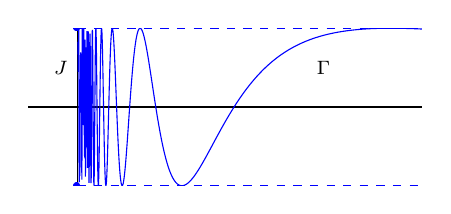
\begin{tikzpicture}
        \begin{axis}[
            axis lines* = middle,
            height=2cm,
            width=5cm,
            scale only axis=true,
            ytick=\empty,
            xtick=\empty,
            xmin=-0.1,
            xmax=0.7,
            ymin=-1,
            ymax=1,
        ]
        \addplot[
            domain=0.001:0.8,
            samples=1000,
            color=blue,
            smooth,
        ]
        {sin(deg(1/x))};
        \draw[blue, dashed] (0,1) -- (1,1);
        \draw[blue, dashed] (0,-1) -- (1,-1);
        \node at (0,0.5) [left] {\scriptsize $J$};
        \node[blue] at (0,1) {\tiny \textbullet};
        \node[blue] at (0,-1) {\tiny \textbullet};

        \node at (0.5, 0.5) {\scriptsize $\Gamma$};
        \end{axis}
        \end{tikzpicture}
        \caption{\textit{Seno del topólogo o de Varsovia.}}
        \label{fig:seno_topologo}
    \end{figure}
\end{enumerate}
\end{ej}

\section{Tabla de comportamiento}%
\label{sec:tabla_de_comportamiento_conx}
En este apartado estudiamos como comporta conexión con respecto a las construcciones del tema \nameref{cha:construcciones}. Se trata de ver cuándo se conserva, cuándo no y qué hipótesis podemos añadir para que se conserve en los casos que no.

\begin{table}[H]
\centering
\begin{tabular}{| c | c | c | c | c |}
\hline
& Subespacios & Cocientes & Productos & Sumas\\
\hline
    Conexión & \ding{55} & \checkmark & \checkmark & \ding{55} \\
    \hline
    Demostración: & $\{0, 1\} \subset \left[ 0, 1 \right]$ & Mantra $2$ & Pivote & Cada sum. es ab. y cerr.\\
    \hline
\end{tabular}
\caption{\textit{Tabla de comportamiento de la conexión con respecto a las construcciones.}}
\end{table}

\begin{prop}
$X \times Y$ conexo $\Leftrightarrow X$ y $Y$ conexo.
\end{prop} 
\begin{demo}
\begin{itemize}
    \item[$\Rightarrow)$] Cada factor es imagen del total a través de la función proyección, que es continua. Como el total es conexo, la imagen continua a través de un conexo es conexa, luego se tiene el resultado.

    \item[$\Leftarrow)$] Fijamos un valor $a \in X$ y entonces vemos que el conjunto
    \[
    Z_y = \underbrace{\left( X \times \{y\} \right)}_{\approx X}\cup \underbrace{\left( \{a\} \times Y \right)}_{\approx Y}
    \]
    es conexo por ser dos conexos que se cortan en el punto $\left( a, y \right)$ (teorema del pivote).
    
    Además, la intersección de todos los $Z_y$
    \[
    \bigcap_{y \in Y} Z_y = \{a\} \times Y \neq \emptyset
    \]
    es no nula, luego por el teorema del pivote de nuevo, tenemos que:
    \[
    \bigcup_{y \in Y} Z_y = X \times Y \text{ conx.}
    \]
    \begin{figure}[H]
        \centering
        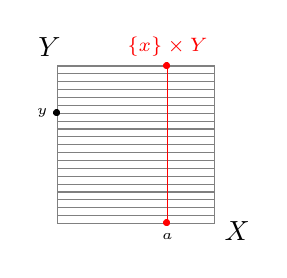
\begin{tikzpicture}
            \draw[gray] (0,0) rectangle (2,2);
            \foreach \y in {0.1, 0.2, ..., 2}
                {
                    \draw[gray,-] (0,\y) -- (2,\y);
                }
            \node at (0,1.4) {\tiny\textbullet};
            \node at (0,1.4) [left] {\tiny $y$};

            \node[red] at (1.4,0) {\tiny\textbullet};
            \node at (1.4,0) [below] {\tiny $a$};

            \draw[red,-] (1.4,0) -- (1.4,2);
            \node[red] at (1.4,2) {\tiny\textbullet};
            \node[red] at (1.4,2) [above] {\scriptsize $\left\{ x \right\} \times Y$};

            \node at (-0.1,2) [above] {$Y$};
            \node at (2,-0.1) [right] {$X$};
        \end{tikzpicture}
        \caption{\textit{Representación de que el producto conexos es conexo: cada línea del cuadrado es un $X \times \left\{ y \right\}.$}}
    \end{figure}
\end{itemize}
\end{demo}


\chapter{Componentes conexas y\texorpdfstring{\\}{} conexión local}%
\label{cha:componentes_conexas_y_conexion_local}
Una vez estudiada la noción de conexión, vamos a repetir el procedimiento que venimos haciendo varios capítulos atrás y vamos a estudiar la versión local de la propiedad. Además, es de especial interés estudiar unos subespacios especiales en cuanto a conexión se refiere que son las componentes conexas y que permiten dividir el espacio en una partición de conjuntos conexos.

\section{Componentes}%
\label{sec:componentes}
Cuando un conjunto no es conexo, tiene sentido preguntarse en cada punto ¿cuál será el mayor subespacio que contiene al punto y que sí es conexo? Porque trabajar en dicho subespacio cuando estemos trabajando en entornos del punto permitirá trabajar como si de un conexo se tratara. Además, este mismo subespacio será el mayor conexo que contiene también a otros puntos distintos, luego en cierta manera podemos verlo como una ``clase de equivalencia'' que asocia puntos con el mismo subespacio conexo maximal.

\begin{defi}[Componente Conexa]
Sea $X$ un espacio topológico, definimos una \textbf{componente conexa} de dicho espacio como un subespacio conexo maximal.
\end{defi}

Aunque la definición anterior es correcta y va en la línea de la intuición explicada al comienzo de la sección, necesitamos formalizar de alguna forma como se calculan dichas componentes conexas cuando nos dan un punto concreto. Esto nos va a permitir no sólo calcular la componente conexa a la que pertenece un punto, sino caracterizar las propiedades que éstas pueden tener dentro del espacio topológico.

\begin{prop}[Caracterización de componentes conexas]
Sea $X$ un espacio topológico y $a\in X$ un punto del mismo, el conjunto:
\[
C(a) := \bigcup_{C \ni a} C \mbox{ donde }C \mbox{ es conexo}
\]
verifica las siguientes propiedades:
\begin{itemize}
\item Es conexo
\item Para cualquier $E\subset X$ conexo tal que $C(a) \cap E \neq \emptyset$, se cumple que $E \subset C(a)$.
\end{itemize}
por tanto, podemos decir que $C(a)$ es la componente\footnote{Puesto que si verifica las dos propiedades mencionadas, entonces es un subespacio conexo maximal.} conexa a la que pertenece $a$.
\end{prop}
\begin{demo}
En primer lugar, como la intersección de todos los conexos de la unión es no vacía (porque $a$ está contenido en la misma) y todos son conexos, por el teorema del pivote el conjunto $C(a)$ es conexo.

Por otro lado, si escogemos un conexo $E\subset X$ tal que $C(a) \cap E \neq \emptyset$, por el teorema del pivote, el conjunto $W := C(a)\cup E$ es conexo y contiene a $a$. Precisamente por esto último, este conjunto es uno de los de la unión que definía $C(a)$, luego $W \subset C(a) \Rightarrow E\subset E \cup C(a) \subset C(a)$, es decir, $E\subset C(a)$.
\end{demo}

\begin{obs}
Tras la caracterización anterior, hay un par de observaciones que son evidentes:
\begin{itemize}
\item Las componentes conexas de dos puntos distintos $a \neq b$ son la misma o son disjuntas, pues si la intersección es no vacía la una está contenida en la otra y viceversa, es decir, son la misma.
\item Como se trata de un conjunto conexo, sabemos que la adherencia $\overline{C(a)}$ es un conjunto conexo. Sin embargo, como $\overline{C(a)}$ es un conjunto conexo que contiene a $a$, tiene que estar contenido en $C(a)$, luego $\overline{C(a)} \subset C(a) \Rightarrow C(a) = \overline{C(a)}$.
\end{itemize}
Las dos observaciones anteriores sumadas a la caracterización, permiten darse cuenta de que el espacio $X$ se puede escribir como unión disjunta
\[
X = \bigsqcup_{C\subset X} C \mbox{ donde }C \mbox{ es comp. conexa}
\]
es decir, que $X$ es una partición de cerrados conexos y disjuntos.
\end{obs}

\begin{ej}
\begin{enumerate}
    \item $X_{\text{discreto}}: C\left( x \right) = \{x\}$ (puntos abiertos y cerrados)
    \item $\mathbb{Q}_u : C\left( p \right) = \{p\}$ (todo intervalo de $\mathbb{R}$ tiene racionales)
    \item $\left( \mathbb{R}, \mathcal{T}_{[, )} \right): C\left( t \right) = \{t\}$ ($\mathbb{R} = \left( \leftarrow, a \right) \cup \left[ a, \rightarrow \right)$ abierto y cerrado)
    \item $X = \{0, Y_k,\ k \ge 1\} : \begin{cases}
        C\left( 0 \right) = \{0\} \text{ cerrado, no abierto} \left( \{\frac{1}{k}: k\ge 1 \}  \text{ no cerr.}\right)\\
        C\left( \frac{1}{k} \right) = \{\frac{1}{k}\} \text{ cerrado y abierto.} 
    \end{cases} $
\end{enumerate}
\end{ej}

\begin{defi}[Espacio totalmente disconexo]
Sea $X$ un espacio topológico, decimos que es \textbf{totalmente disconexo} si y sólo si $\forall a \in X : C(a) = \{a\}$ o, lo que es lo mismo, las componentes conexas del conjunto son los puntos.
\end{defi}

\begin{prop}
Sean $X$ e $Y$ espacios topológicos y $X\times Y$ el espacio topológico producto, las componentes conexas de $X \times Y$ son los productos de componentes conexas de $X$ y de $Y$.
\end{prop}
\begin{demo}
\begin{itemize}
\item $\Rightarrow $ Las componentes conexas del producto son producto de componentes conexas.

Sea $C \subset X \times Y$ una componente conexa del producto, si denotamos por $p$ y $q$ a las proyecciones sobre cada factor, entonces $p\left( C \right)$ y $q\left( C \right)$ son conexos en $X$ e $Y$ respectivamente (por ser imagen continua de conexo). Estos conexos estarán a su vez contenidos en alguna componente conexa del factor de forma que:
\[
\begin{cases}
    p\left( C \right) \subset E \stackrel{\text{c.c}}{\subset}  X\\
    q\left( C \right) \subset F \stackrel{\text{c.c}}{\subset}  Y
\end{cases} \Rightarrow C \subset E \times F \mbox{ donde } E \times F \mbox{ es conexo}
\]
y como $C$ es un subespacio conexo maximal, necesariamente debe ocurrir que $C = E\times F$.

\item $\Leftarrow$ El producto de componentes conexas es una componente conexa

Supongamos que tenemos dos componentes conexas $C_x$ y $C_y$ de $X$ e $Y$ respectivamente y que $\exists E \subset X$ conexo tal que $E\cap C_x \times C_y \neq \emptyset$, pero $E \not\subset C$. Como $E\cap C_x \times C_y \neq \emptyset$, por el teorema del pivote, $E\cup C_x \times C_y$ es conexo. La proyección $p(E\cup C_x \times C_y)$ es el conjunto conexo formado por los valores $x\in X : x\in E_x \ \vee \ x\in C_x$ y como $C_x \subset p(E\cup C_x \times C_y)$ y es conexo maximal, sabemos que $C_x = p(E\cup C_x \times C_y)$. Un razonamiento análogo para $q$ revela que $C_y = q(E\cup C_x\times C_y)$. Por tanto, hemos conseguido que $E\cup C_x\times C_y = C_x \times C_y$, es decir, que $E\subset C_x \times C_y$, luego absurdo.
\end{itemize}
\end{demo}

\section{Conexión local}%
\label{sec:conexion_local}
En ocasiones es muy útil poder tener la certeza de que puedo trabajar en cada punto de forma local sabiendo que se cumple cierta propiedad. Para ello, vamos a definir qué significa ser conexo localmente y cómo puede esta definición ayudar a satisfacer la cuestión mencionada.

\begin{defi}[Localmente Conexo]
Sea $X$ un espacio topológico, decimos que es \textbf{localmente conexo} si y sólo si para todo punto $x \in X$ existe una base de entornos $\mathcal{B}^x$ formada por entornos abiertos conexos.
\end{defi}

\begin{prop}[Caracterización de conexión local]
Sea $X$ un espacio topológico, este es localmente conexo si y sólo si las componentes conexas de un abierto son abiertas.
\end{prop}
\begin{demo}
\begin{itemize}
    \item[$\Rightarrow)$] 
    
	Vamos a ver que las componentes conexas son entornos de todos sus puntos. Para ello, consideremos $x \in C \stackrel{\text{c.c}}{\subset} U \ab X$. Como $X$ es localmente conexo, con seguridad existirá un $U^x \ab X$ conexo y contenido en $U$ (porque como hay una base de entornos de abiertos conexos, $U$ debe contener alguno). La conexión de $U^x$ implica que $U^x \subset C$ por ser esta componente conexa, luego acabamos de demostrar que $C$ es entorno de todos sus puntos, es decir, abierto. 
	
    \item[$\Leftarrow)$]
    
    Dado un punto $x\in X$, basta con que escojamos como base de entornos las componentes conexas de los abiertos que contienen al punto
    \[
    \mathcal{B}^x := \{C\left( x \right) \stackrel{\text{c.c}}{\subset} U \ab X : x \in U\}			\]
    Dicho conjunto es base de entornos porque cada $C(x)$ es entorno (por ser abierta) y cualquier otro entorno debe contener a alguna, puesto que por ser entorno contendrá algún abierto que contenga al punto y, en consecuencia, alguna de las componentes conexas del conjunto.
\end{itemize}
\end{demo}

\begin{obs}
Sin muchísima dificultad, es sencillo demostrar que la definición de conexión local puede prescindir de la apertura de los conexos que forman la base de entornos, esto es, que la definición dada es equivalente a: ``$X$ es localmente conexo si y sólo si $\forall x \in X,\ \exists \mathcal{V}^x$ base de entornos conexos''.
\end{obs}

\begin{ej}[Esencial]
$\{0, \frac{1}{k} : k \ge 1\} = Y \subset \mathbb{R}_u$ \underline{no} es localmente conexo. 
\begin{demo}
    La $\text{c.c}\left( 0 \right) = \{0\}$ no es abierto. Directamente:
    \begin{align*}
        0 \in \underbrace{V}_{\text{ent. de } 0 \in \mathbb{R}} \cap Y &\Rightarrow V \supset \left( 0, \varepsilon \right),\ \exists 0 < \underbrace{\theta}_{\not\in \mathbb{Q}} < \frac{1}{k} < \varepsilon < 1\\
        &\Rightarrow V\cap Y \subset \underbrace{\left( \leftarrow, \theta \right)}_{\ni 0} \cup \underbrace{\left( \theta, \rightarrow \right)}_{\ni \frac{1}{k}}  \Rightarrow V \cap Y \text{ no conexo.} 
    .\end{align*}
\end{demo}
\end{ej}

\begin{ej}
Supongamos que tenemos un conjunto de segmentos verticales que convergen al segmento de la izquierda del todo, que también incluimos en el conjunto, tal y como muestra la figura
    \begin{figure}[H]
        \centering
        \begin{tikzpicture}
            \foreach \x in {0, 0.005, 0.01, 0.02, 0.035, 0.1, 0.25, 0.5, 0.8, 1.5, 3, 6}
                \draw[-, gray] (\x, 0) -- (\x, 2);
        \end{tikzpicture}
        \caption{\textit{Ejemplo}}
    \end{figure}
¿Es este conjunto localmente conexo? La respuesta es no. Para ver esto, tenemos que ver que para cada punto existe una base de entornos formada por abiertos conexos. En cualquier segmento que no sea el de la izquierda del todo, podemos encontrar una bola $B(x,\rho)$ con $\mathbb{\rho}$ real tal que dicha bola no interseque con ningún otro segmento del conjunto, luego la colección $\{B(x,\varepsilon) : 0 < \varepsilon < \rho\}$ es una base de entornos de cualquier punto de estos segmentos. El problema principal está en el segmento de la izquierda del todo, pues cualquier bola $B(x,\rho)$ centrada en dichos puntos necesariamente interseca con muchos otros segmentos (porque los segmentos convergen hacia la izquierda). Con esto hemos demostrado que cualquier entorno de uno de estos puntos, necesariamente contiene puntos de otros segmentos y entonces el entorno inicial siempre será disjunto.
\end{ej}

\section{Tabla de comportamiento}%
\label{sec:tabla_de_comportamiento_loc_conx}
En este apartado estudiamos como se comportan la conexión local con respecto a las construcciones del tema \nameref{cha:construcciones} para ver cuándo se conservan, cuándo se pierden y qué podemos añadir para no perderlas.

%TODO: Fix tabla. En subespacios los abiertos sí heredan
\begin{table}[H]
\begin{tabular}{| c | c | c | c | c |}
\hline
& Subespacios & Cocientes & Productos & Sumas\\
\hline
Conexión local & \begin{tabular}{cc} \ding{55} & $\checkmark_{abierto}$ \end{tabular} & \checkmark & \begin{tabular}{cc} \checkmark & \checkmark \end{tabular} & \begin{tabular}{cc} \checkmark & \checkmark \end{tabular} \\
\hline
Demostración: & Ejemplo esencial & No banal & Prod. ent. conx. & Suma como sum's\\
\hline
\end{tabular}
\caption{\textit{La tabla nos indica como se conserva la compacidad local en las construcciones que hemos visto. Las sumas y los productos son finitos.}}
\end{table}


\begin{prop}
Sea $X$ un espacio topológico localmente conexo y $f : X \rightarrow Y$ una identificación a un espacio $Y$, el espacio $Y$ es localmente conexo.
\end{prop}
\begin{demo}
Para demostrar la local conexión, vamos a demostrar que las componentes conexas de abiertos son abiertas. Para ello, tomemos un abierto $V\ab Y$ y una componente conexa suya $C \subset V$ y veamos que tiene que ser abierta.

\begin{center}
        \includegraphics[scale=0.3]{images/dem_loc_conx_loc_conx} 
\end{center}

En primer lugar, por la continuidad de $f$, $f^{-1} V \ab X$ así que la local conexión de $X$ nos asegura que $\exists U^x \ab f^{-1}V$ pero además este es conexo. Como $f$ es continua, $f(U^x)$ es conexo y contiene a $x$, luego por la maximalidad de $C$ debe ocurrir que $f(U^x)\subset C$. Por tanto, ahora vemos con facilidad que $f^{-1} C \subset f^{-1}V$ contiene a $U^x$, es decir, hemos visto que la preimagen $f^{-1}C$ es abierta en $X$ y como es abierto saturado $C$ es abierto.
\end{demo}

\chapter{Conexión por caminos}%
\label{cha:conexion_por_caminos}
La conexión por caminos va a ser un elemento central sobre todo en la parte de topología algebraica posterior. Es similar al concepto de conexión que hemos visto, pero la diferencia es que introducimos un elemento ``conector'': los caminos.

\begin{defi}[Camino]
Sea $X$ un espacio topológico, definimos un \textbf{camino en $X$} como una aplicación continua $\alpha: \left[ a, b \right] \subset \mathbb{R}_u \rightarrow X$ y decimos que:
\begin{itemize}
    \item Los puntos $\alpha\left( a \right)$ y $\alpha\left( b \right)$ son los extremos inicial y final del camino.
    \item La imagen $\alpha\left[ a, b \right] \subset X$ es\footnote{Nótese que la traza es un conexo, pues es imagen continua del conexo $[a,b]$.} la \textbf{traza}.
\end{itemize}
\end{defi}

\begin{prop}[Cambios de parámetros]
Sea $X$ un espacio topológico, $\alpha :[a,b] \rightarrow X$ un camino en él y $\varphi
 : [c,d]\rightarrow [a,b]$ una aplicación, entonces:
\begin{itemize}
\item Si $\varphi$ es continua, la aplicación $\alpha \circ \varphi :[c,d]\rightarrow X$ es otro camino sobre $X$ con la misma traza que $\alpha$.
\item Si $\varphi$ es un homeomorfismo\footnote{En funciones de un variable, la equivalencia a ser homeomorfismo (biyectiva, continua y continua la inversa) es ser una función continua y monótona.}, la aplicación $\alpha \circ \varphi:[c,d]\rightarrow X$ es exactamente el mismo camino que $\alpha$, pero con parametrización distinta.
\end{itemize}
al último resultado se le conoce como \textbf{cambio de parámetro}. 
\end{prop}

\begin{obs}
Es importante tener en cuenta que sólo se trata del mismo camino cuando $\varphi$ es homeomorfismo. La principal diferencia está en que cuando $\varphi$ es sólo continua, se conserva la traza, pero no la velocidad a la que se recorre.
\end{obs}

\begin{ej}
Un cambio de parámetro muy útil en lo que queda de documento va a ser la interpolación lineal, que consiste en la parametrización de cualquier segmento en términos del segmento $[0,1]$. El cambio, considerando $p, q\in \mathbb{R}^n$, viene dado por la siguiente aplicación:
\begin{align*}
\varphi : [0, 1] &\longrightarrow [p, q] \\
			t & \longmapsto (1-t)p + tq
\end{align*}
Este resultado es muy potente porque permite reducir cualquier camino a uno parametrizado en $[0,1]$, lo que será de gran utilidad en los capítulos posteriores.
\end{ej}

\begin{defi}[Producto de caminos]
Sea $X$ un espacio topológico y $\alpha : [a,b]\rightarrow X$ y $\beta:[c,d]\rightarrow X$ dos caminos tales que $\alpha(b) = \beta(c)$, entonces la aplicación:
\begin{align*}
\alpha \ast \beta : [a,b] \cup [c,d] &\longrightarrow X \\
						t &\longmapsto \begin{cases}
										\alpha(t) & t \in [a,b] \\
										\beta(t) & t\in [c,d]
										\end{cases}	
\end{align*}
es el camino que resulta de unir los caminos $\alpha$ y $\beta$.
%TODO: Imagen
\begin{center}
    \includegraphics[scale=0.3]{images/prod_caminos} 
\end{center}
\end{defi}

\begin{obs}
Una alternativa para ver mejor que se trata de un camino es reparametrizar el camino $\beta$ al intervalo $[b,b+(d-c)]$. Como $\beta(b) = \alpha(b)$, el camino $\alpha \ast b$ definido en $[a,b+(d-c)]$ ahora ya tiene un aspecto más uniforme que el de la definición.
\end{obs}

\begin{ej}
Si hacemos el producto de segmentos consecutivos obtenemos \textbf{caminos poligonales}. 
\end{ej}

\section{Mantras y propiedades}%
\label{sec:conexion_por_caminos}
Una vez definidos los conectores fundamentales que serán los caminos, ahora sí podemos estudiar qué significa estár conectado por caminos y qué consecuencias tiene con respecto a la conexión y las propiedades del espacio.

\begin{defi}[Conexión por caminos]
Sea $X$ un espacio topológico, decimos que es \textbf{conexo por caminos} si y sólo si 
\[
\forall x, y \in X,\ \exists \sigma: \left[ a, b \right] \rightarrow X,\ \sigma\left( a \right) = x\; \land \;\sigma\left( b \right) = y
\]
cualesquiera dos de sus puntos se pueden conectar con un camino.
\end{defi}

\begin{obs}
Fijemos un $x_0\in X$ y consideremos $\sigma_x : [a,b]\rightarrow X$ tal que $\sigma_x(a) = x_0$ y $\sigma_x(b) = x$. Como la traza de $\sigma_x$ hemos comentado que es conexa y podemos escribir\footnote{En este caso, $\sigma_x$ es un abuso de notación para escribir que es la traza de $\sigma_x$.} $X = \bigcup_{x\in X} \sigma_x$, el conjunto $X$ es conexo por el teorema del pivote (pues todos los $\sigma_x$ intersecan en $x_0$).
\end{obs}

\begin{ej}
\begin{enumerate}
    \item La mayor parte de los conexos conocidos son conexos por caminos:
    \begin{itemize}
        \item Los abiertos conexos de la topología usual son conexos por poligonales, que son caminos.
        \item Los conjuntos convexos y los estrellados también son conexos (casi por definición se prueba).
    \end{itemize}
    \item El seno del topólogo $\Gamma$ es la traza de $\alpha\left( t \right) = \left( t, \sin\frac{1}{t} \right) : t > 0$ y es conexo tanto él como su adherencia $\overline{\Gamma} = J \cup \Gamma$ donde $J = \{0\} \times \left[ 0, 1 \right]$. Sin embargo, la adherencia $\overline{\Gamma}$ sirve como contraejemplo para ver un conjunto conexo que no es conexo por caminos.
    \begin{demo}
    Fundamentalmente hay que demostrar que no todos los puntos están conectados por caminos. En particular, vamos a demostrar que no existen caminos que $\sigma: \left[ a, b \right] \rightarrow \overline{\Gamma}$ donde $\sigma\left( a \right) = p \in J$ y $\sigma\left( b \right) = q \in \Gamma$, es decir, al intentar buscar un camino de $J$ a $\Gamma$ la cosa se estropea.
    	\begin{center}
            \includegraphics[scale=0.3]{images/dem_sin_top_no_conx_caminos} 
        \end{center}
	Supongamos que sí, que existe un camino con $\sigma(0) = p \in J$ y $\sigma(1) = q \in \Gamma$ definido como:
	\begin{align*}
		\sigma : [0, 1] &\longrightarrow \overline{J} \\
					t &\longmapsto (\alpha(t), \beta(t))
	\end{align*}
	entonces el valor $t_0 = \max \{t \in \left[ a, b \right] : \alpha\left( t \right) = 0\}$ existe porque (falta explicación) y es menor estricto que $1$, pues $\sigma(1) = (\alpha(1), \beta(1)) = q \in J \Rightarrow \alpha(1) \neq 0$. Al valor $\sigma(t_0) = (0, \beta(t_0))$ lo denotaremos por $p'$ en lo sucesivo.
	
	   $\Rightarrow \begin{cases}
                \alpha\left( a' \right) = 0,\ \sigma\left( a' \right) = p' \in J\\
                t > a': \alpha\left( t \right) > 0 \Rightarrow \sigma\left( t \right) \in \Gamma \Rightarrow \beta\left( t \right) = \sin \frac{1}{\alpha\left( t \right)} 
            \end{cases} $

            Supongamos $p' = \sigma\left( a' \right) \neq \left( 0, 1 \right)$ (punto) y $\exists \delta: B\left( p', \delta \right) \cap \{y = 1\} = \emptyset$. $\sigma$ continua $\Rightarrow \exists \sigma\left[ a', \varepsilon \right] \subset B\left( p', \delta \right) \Rightarrow \sigma\left[ a', \varepsilon \right] \cap \{y = 1\} = \emptyset$. (si $p' = \left( 0, 1 \right)$ evitaríamos $\{y = -1\}$)

            $\alpha$ continua $\Rightarrow \alpha\left[ a', \varepsilon \right] \subset \mathbb{R}$ conexo compacto $=$ intervalo: $\alpha\left[ a', \varepsilon \right] = \left[ 0, c \right]$.

            La oscilación de $\sin \frac{1}{x}$ lleva $\sigma$ a $\{y = 1\}$, fuera de la bola elegida:
            \begin{align*}
            k \gg 0 &\Rightarrow \frac{2}{\left( 1 + 4k \right) \pi} \in \left[ 0, c \right] = \alpha\left[ a', \varepsilon \right] \Rightarrow \exists a' < t_k < \varepsilon: \alpha\left( t_k \right) = \frac{2}{\left( 1 + 4k \right) \pi}\\ 
                &\Rightarrow \sigma\left( t_k \right) = \left( \alpha\left( t_k \right), \sin\left( \frac{1}{\alpha\left( t_k \right)} \right) \right) = \left( x_k, 1 \right) 
            \bot \end{align*}
    \end{demo}
\end{enumerate}
\end{ej}

Como el concepto también tiene que ver con la conexión de un conjunto y parece muy similar al que hemos comentado, parece razonable que casi todo lo que dijimos acerca de conexión sea válido en este caso.

\begin{theo}[del pivote]
Sea $X$ un espacio topológico, $A$ un subespacio definido como $A = \bigcup_{i} A_i$ donde los $A_i$ son una familia de conexos por caminos de $X$, si $\bigcap_{i} A_i \neq \emptyset$, entonces $A$ es conexo por caminos. 
\end{theo}
\begin{demo}
\begin{center}
    \includegraphics[scale=0.3]{images/dem_pivote_caminos} 
\end{center}
\end{demo}

\begin{theo}[Conservación por continuidad]
Sean $X$ e $Y$ espacios topológicos, $f: X \rightarrow Y$ una función continua y $A \subset X$ un conjunto conexo por caminos, entonces $f\left( A \right)$ es conexo por caminos.
\end{theo}
\begin{demo}
\begin{center}
    \includegraphics[scale=0.3]{images/dem_imagen_caminos} 
\end{center}
\end{demo}

\begin{obs}
Uno podría pensar, por la similitud que estamos viendo con la conexión del capítulo anterior, que el teorema sobre la conexión de la adherencia es extensible a la conexión por caminos. Sin embargo ¡Esto no es cierto!

El seno del topólogo $\Gamma$ es conexo por caminos: $\left( a, \sin\frac{1}{a} \right)$ y $\left( b, \sin\frac{1}{b} \right)$ se conectan por el camino evidente, $\alpha\left( t \right) = \left( t, \sin\frac{1}{t} \right),\ a \le t \le b$. Pero, como hemos visto, la adherencia $\overline{\Gamma}$ no es conexa por caminos. 
\end{obs}

\section{Tabla de comportamiento}%
\label{sec:tabla_de_comportamiento_conx_caminos}
En este apartado estudiamos como se comportan la conexión por caminos con respecto a las construcciones del tema \nameref{cha:construcciones} para ver cuándo se conservan, cuándo se pierden y qué podemos añadir para no perderlas.

%TODO: Fix tabla
\begin{table}[H]
\centering
\begin{tabular}{| c | c | c | c | c |}
\hline
& Subespacios & Cocientes & Productos & Sumas\\
\hline
Conexión por caminos & \ding{55} & \checkmark & \begin{tabular}{cc} \checkmark & \checkmark \end{tabular} & \ding{55} \\
\hline
Demostración: Conexo & Continuidad & Prop & ??? \\
\hline
\end{tabular}
\caption{\textit{La tabla nos indica como se conserva la conexión por caminos en las construcciones que hemos visto. Las sumas y los productos son finitos.}}
\end{table}

\begin{prop}[Conservación por producto]
Sean $X$ e $Y$ dos espacios topológicos, el producto $X\times Y$ es conexo por caminos si y sólo si $X$ e $Y$ son conexos por caminos.
\end{prop}
\begin{demo}
\begin{itemize}
\item $\Leftarrow$

Escojamos dos puntos cuales quiera $\left( x_1, y_1 \right),\ \left( x_2, y_2 \right) \in X \times Y$ y veamos que existe un camino que los une. Por la conexión por caminos de cada componente del producto, sabemos que ocurre lo siguiente: 
\[
\begin{cases}
    \sigma: \left[ a, b \right] \rightarrow X: \begin{cases}
        \sigma\left( a \right) = x_1 \\
        \sigma\left( b \right) = x_2
    \end{cases} \\
    \tau: \left[ a, b \right] \rightarrow Y: \begin{cases}
        \tau\left( a \right) = y_1 \\
        \tau\left( b \right) = y_2
    \end{cases}
\end{cases} 
\]
Luego la composición de ambos caminos sobre cada componente como componentes de un camino en el producto necesariamente será un camino que unirá los puntos del inicio.
\[
\gamma = \left( \sigma, \tau \right) : \left[ a, b \right] \rightarrow X \times Y: \begin{cases}
        \gamma\left( a \right) = \left( x_1, y_1 \right)\\
        \gamma\left( b \right) = \left( x_2, y_2 \right)
    \end{cases}  
\]

\item $\Rightarrow$

Como para que una función con varias componentes sea continua cada componente debe ser continua, el proceso de la implicación anterior es completamente reversible porque la existencia de un camino en el producto implica la existencia de un camino en cada componente considerando dicha componente como camino en el factor.
\end{itemize}
\end{demo}


\chapter{Componentes conexas\texorpdfstring{\\}{} por caminos y conexión\texorpdfstring{\\}{} local por caminos}%
\label{cha:componentes_conexas_por_caminos_y_conexion_local_por_caminos}
Del mismo modo que estudiamos en el capítulo de conexión las ``piezas conexas'' en las que se podían dividir los conjuntos que no eran conexos y localizamos la noción de conexión, tiene sentido definir los mismos conceptos para conexión local.

\section{Componentes conexas por caminos}%
\label{sec:componentes_conexas_por_caminos}
La definición y las propiedades de las componentes conexas por caminos serán prácticamente iguales a las de conexión salvo por algún detalle menor. El fundamento de la idea, que es la de subconjunto conexo maximal, sigue siendo el componente básico de la teoría.

\begin{defi}[Componente conexa por caminos]
Sea $X$ un espacio topológico, definimos una \textbf{componente conexa por caminos} como un subconjunto conexo por caminos maximal.
\end{defi}

\begin{prop}[Caracterización de componentes conexas por caminos]
Sea $X$ un espacio topológico y $a\in X$ un punto del mismo, el conjunto:
\[
C_c(a) := \bigcup_{A \ni a} A \mbox{ donde }A \mbox{ es conexo por caminos}
\]
verifica las siguientes propiedades:
\begin{itemize}
\item Es conexo por caminos
\item Para cualquier $E\subset X$ conexo por caminos tal que $E\cap C_c(a) \neq \emptyset$, se cumple que $E\subset C_c(a)$.
\end{itemize}
\end{prop}
\begin{demo}
Si uno se fija en la demostración de la misma proposición para componentes conexas, se dará cuenta que principalmente la herramienta que utiliza es el teorema del pivote y, como hemos demostrado dicho teorema para la conexión por caminos, la demostración es completamente análoga.
\end{demo}

\begin{obs}
De la misma forma que las componentes conexas formaban una partición de $X$, las componentes conexas por caminos formarán una partición de $X$ ¡pero más fina y no necesariamente de cerrados! De nuevo, el seno del topólogo es un buen contraejemplo: si consideramos el espacio $X = \overline{\Gamma}$, los conjuntos $J$ y $\Gamma$ son dos componentes conexas por caminos donde la primera es cerrada y la otra no. Además, $\overline{\Gamma}$ sólo tiene una componente conexa (ella misma), pero acabamos de ver que tiene dos componentes conexas por caminos, luego la partición es más fina.
\end{obs}

\section{Conexión local por caminos}%
\label{sec:conexion_local_por_caminos}
En este caso, también es útil conocer cuándo podemos trabajar de forma local a un punto asumiendo que dicha localización es conexa por caminos y a esto es lo que llamamos conexión local por caminos.

\begin{defi}[Conexión local por caminos]
Sea $X$ un espacio topológico, decimos que es \textbf{localmente conexo por caminos} si y sólo si para todo punto $x\in X$ existe una base de entornos $\mathcal{B}^x$ formada por abiertos conexos por caminos.
\end{defi}

\begin{prop}[Caracterización de la conexión local]
Sea $X$ un espacio topológico, $X$ es localmente conexo por caminos si y sólo si las componentes conexas por caminos de un abierto son abiertas.
\end{prop}
\begin{demo}
De nuevo, las demostraciones son completamente análogas a sus homólogas del capítulo de conexión.
\end{demo}

\begin{obs}
Sin excesiva dificultad, es sencillo demostrar que la definición de conexión local puede prescindir de la apertura de los conexos que forman la base de entornos, esto es, que la definición dada es equivalente a ``$X$ es localmente conexo por caminos si y sólo si $\forall x \in X, \ \exists \mathcal{V}^x$ base de entornos formada por conexos por caminos''
\end{obs}

\section{Tabla de comportamiento}%
\label{sec:tabla_de_comportamiento_conx_local_caminos}
%TODO: Fix tabla
\begin{table}[H]
\centering
\begin{tabular}{| c | c | c | c | c |}
\hline
& Subespacios & Cocientes & Productos & Sumas\\
\hline
Conexión local por caminos & \ding{55} & \checkmark & \checkmark & \checkmark\\
\hline
\end{tabular}
\caption{\textit{También vale que las c.c.c del producto son los productos de las c.c.c de los factores.}}
\end{table}

\section{Relaciones entre las propiedades de conexión}%
\label{sec:relaciones_entre_las_propiedades_de_conexion}
Por las similitudes entre ambos tipos de conexión definidos, no está demás estudiar qué condiciones han de darse para obtener unas a partir de otras y viceversa.

\begin{prop}
Conexo y localmente conexo por caminos $\Rightarrow$ Conexo por caminos.
\end{prop}
\begin{demo}
\begin{itemize}
    \item Conexo $\Rightarrow \forall x, y,\ \exists \text{ cadenas de } x \text{ a } y$.
    \item Localmente conexo por caminos $\Rightarrow$ cadenas de abiertos conexos por caminos $\xRightarrow{\text{Variante del pivote}}$ Estas cadenas son conexas por caminos.
\end{itemize}
Por tanto, $\exists$ camino de $x$ a $y$.
\end{demo}

\begin{obs}[Resumen]
Por especificar todas las posibilidades:
%TODO: Imagen
\begin{center}
    \includegraphics[scale=0.3]{images/resumen_conx} 
\end{center}
\end{obs}

\begin{enun}
Contraejemplos. Los menos fáciles son $*$ y $**$ 
\end{enun}

\begin{ej}
\begin{itemize}
    \item Sea $\left( \mathbb{R}^2, \mathcal{T}_{\text{rad}} \right)$. Veamos si es conexo por caminos porque entonces será conexo.

    %TODO: Dibujo
    Primero intentamos parametrizar por interpolación: $\left( 1 - t \right)a + tb$. Como $\mathcal{T}_{\text{rad}}|_r = \mathcal{T}_{u}|_r$ es correcto el camino ($r$ es una recta).
    En cambio si el camino es una curva cualquiera, la topología relativa es la discreta, es decir, la preimagen de un punto es todo $\left[ 0, 1 \right]$ al ser 
    un abierto y cerrado en un conexo. Por tanto, $f$ será constante (contradicción).

    En definitiva, tomamos como caminos entre dos puntos, la recta que los une. Con esto, el espacio es conexo por caminos $\Rightarrow$ conexo.

    La usual es localmente conexa por caminos. Si en la radial es localmente conexa por caminos tenemos que si $x_0 \in U$ entonces $\exists U \supset V_{\text{ab}} = C_{\text{cam.}} \left( x_0 \right)$es el candidato a entorno abierto conexo por caminos de la base buscada. 

    Usaremos $V = \left\{ x \in U : \exists P \supset U: x_0 \rightarrow x\right\}$ con $P$ poligonal %TODO: Dibujo
    que será conexo por caminos radiales. Veamos que es abierto (radial).

    Esto quiere decir que $\forall x \in V$ se cumple ``la condición radial''.
    %TODO: Dibujo
    $\exists \underbrace{\left( x - \varepsilon, x + \varepsilon \right)}_{\ni y} \subset U \cap L$. Formamos $P_y = P_x \cup \left[ x, y \right] \subset U \Rightarrow \left( x - \varepsilon, x + \varepsilon \right) \subset V \cap L$.

    %TODO: Cambiar de lugar
    \item Veamos ahora la compacidad tenemos que $\mathcal{T}_u \subset \mathcal{T}_r \Rightarrow$ si $K$ compacto en la radial $\Rightarrow$ también lo será en la usual. Por tanto, al no ser $\mathbb{R}^2$ con la usual compacto, tampoco lo será con la radial.

    En cambio como con la usual, $\mathbb{R}^2$ sí es Lindelöf no podemos decidir directamente si con la radial lo es o no. Pero no es así porque las curvas son cerradas pero su topología relativa es la 
    discreta y, por tanto, no son Lindelöf. Como se hereda, la radial no puede ser Lindelöf.

    \item Veamos la compacidad local. No lo es. %TODO: Imagen.
\end{itemize}
\end{ej}


%\part{Topología algebraica}
%\chapter{Homotopía}%
\label{cha:homotopia}
\section{Conceptos fundamentales}%
\label{sec:conceptos_fundamentales}
\begin{defi}
Una \textbf{homotopía} es una aplicación continua $H : Y \times \left[ 0, 1 \right] \rightarrow X$.
\end{defi}
\begin{obs}
\begin{enumerate}
    \item $H_s : Y \rightarrow X: y \mapsto H\left( y, s \right),\ H \equiv \{H_s: 0 \le s \le 1\}$ familia uniparamétrica de aplicaciones.
    \item Siendo $f = H_0$ y $g = H_1$:
    \[
    \begin{cases}
        H_s : f \simeq g \text{, homotopía entre } f \text{ y } g\\
        H \text{ deformación continua de } f \text{ a } g
    \end{cases} 
    \]
    Con esto, el problema que deseamos resolver es ver cuándo dos aplicaciones son \textbf{homótopas}:
    \[
    \boxed{f \simeq g} 
    \]

    \item $f \simeq g$ relación de equivalencia:
    \begin{itemize}
        \item $f \simeq f$ vía $H_s \equiv f$.
        \item $H_s : f \simeq g \Rightarrow H_{1 - s} : g \simeq f$.
        \item $\begin{rcases}
            F_s : f \simeq g\\
            G_s: g \simeq h
        \end{rcases} \Rightarrow H_s = \begin{cases}
            F_{2s},\ 0 \le s \le 1/2\\
            G_{2s - 1}\ 1/2 \le s \le 1
        \end{cases}: f \simeq h$
        \begin{demo}
            Continuidad: $\begin{cases}
            F_{2(1/2)} = F_1 = g\\
            G_{2(1/2) - 1} = G_0 = g
            \end{cases}$. En el resto de puntos la continuidad se da por serlo $F$ y $G$.
        \end{demo}
        Como notación tenemos que $H_s = F_s * H_s$.
    \end{itemize}
\end{enumerate}

Habitualmente tomamos como hipótesis que el espacio sea conexo por caminos y conexo local por caminos.
\end{obs}

\begin{prop}
$X$ conexo por caminos, $f, g: Y \rightarrow X$ constantes $\Rightarrow f \simeq g$.
\end{prop}
\begin{demo}
Por hipótesis tenemos que $f \equiv x_0$ y $g \equiv x_1$. Entonces, como $\exists \sigma: \left[ 0, 1 \right] \rightarrow X,\ \sigma\left( 0 \right) = x_0$ y $\sigma\left( 1 \right) = x_1 \Rightarrow H_s \equiv \sigma\left( s \right) : \begin{cases}
    H_0 \equiv \sigma\left( 0 \right) = x_0 \equiv f\\
    H_1 \equiv \sigma\left( 1 \right) = x_1 \equiv g
\end{cases}$
\end{demo}

\begin{defi}
$f: Y \rightarrow X$ es \textbf{nulhomótopa} si $f \simeq $ constante, \textbf{esencial} en caso contrario.
\end{defi}

\begin{theo}[Problema esencial. Fibración de Hopf]
(1932) $\exists f : \mathbb{S}^3 \rightarrow \mathbb{S}^2$ esencial con $\mathbb{S}^3 \subset \mathbb{R}^4 = \mathbb{C}^2$ y $\mathbb{S}^2 \subset \mathbb{R}^3 = \mathbb{R} \times \mathbb{C}$:
\[
\left( z, z' \right) \mapsto \left( \lVert z \rVert^2 - \lVert z' \rVert^2, 2 z z'\right)
\]
\end{theo}
Este ejemplo es importante porque demuestra que no todas las aplicaciones son nulhomótopas.

\section{Concepto relativo}%
\label{sec:concepto_relativo}
\begin{defi}
$H: Y \times \left[ 0, 1 \right] \rightarrow X$ es una \textbf{homotopía relativa a} $A \subset Y$ si $H_s\left( a \right) = H_0\left( a \right),\ \forall a \in A$ y $\forall s \in \left[ 0, 1 \right]$.
\end{defi}

\begin{prop}
$H$ relativa a $A,\ f = H_0,\ g = H_1 \Rightarrow f|_A = g|_A$. Notación: $H_s = f \stackrel{A}{\simeq} g$ (Relación de equivalencia).
\end{prop}

\begin{ej}[Fundamentales. Interpolación]
\begin{enumerate}
    \item $f, g: Y \rightarrow X \subset \mathbb{R}^n$ convexo $\Rightarrow\exists H_s = \left( 1 - s \right) f + sg: f \simeq g$.
    \begin{demo}
        Pues por convexidad $H_s\left( y \right) \in \underbrace{\left[ f\left( y \right), g\left( y \right) \right] \subset X}_{\text{\textbf{cond. crucial!}}}$.
    \end{demo}
    $f\left( a \right) = g\left( a \right) \Rightarrow H_s\left( a \right) = \left( 1 - s \right)f\left( a \right) + sg\left( a \right) = f\left( a \right) = g\left( a \right) \Rightarrow H_s$ es relativa a $A = \{f = g\}$.

    Con esto vemos que dos funciones continuas en un convexo con homótopas.

    \item $f: Y \rightarrow X \subset \mathbb{R}^n$ estrellado respecto de $x_0,\ \left[ x, x_0 \right] \subset X,\ \forall x \in X \Rightarrow H_s = \left( 1 - s \right)f + sx_0: f \simeq x_0$ (relativa a $A = f^{-1}\left( x_0 \right)$).

    De nuevo, por transitividad, dos funciones continuas en un estrellado son homótopas.

    \item Variante en $\mathbb{S}^n$:
    %TODO: Imagen
    \begin{center}
        \includegraphics[scale=0.3]{images/ej_fund_interp_3} 
    \end{center}
\end{enumerate} 
\end{ej}

\section{Contractibilidad}%
\label{sec:contractibilidad}
\begin{defi}
$X$ es \textbf{contráctil} si $id: X \rightarrow X$ es nulhomótopa: $\exists H_s : id \simeq x_0$.

Y \textbf{fuertemente contrátil} si $\exists H_s : id \stackrel{x_0}{\simeq} x_0$ (homótopa relativa a $\{x_0\}$)
\end{defi}

\begin{obs}
Los ejemplos son difíciles, pero son cosas distintas.
\end{obs}

\begin{ej}
    $X \subset \mathbb{R}^n$ estrellado respecto $x_0 \Rightarrow$ fuertemente contráctil
    \begin{demo}
        $H_s = \left( 1 - s \right) id + sx_0$.
    \end{demo}
\end{ej}

\begin{prop}
\begin{enumerate}
    \item Si $X$ es contrátil $\Rightarrow$ es conexo por caminos.
    \item Si $X$ es contráctil $\Rightarrow \begin{cases}
        \forall f: Y \rightarrow X \text{ nulhomótopa.}\\
        \forall g: X \rightarrow Z \text{ nulhomótopa.} 
    \end{cases} $
\end{enumerate}
\end{prop}
\begin{demo}
\begin{enumerate}
    \item $H_s: id \simeq x_0 \Rightarrow S \mapsto H_s\left( x_0 \right)$ camino de $x$ a $x_0$.
    \item $H_s: id \simeq x_0 \begin{cases}
        H_s \circ f: f \simeq x_0\\
        g \circ H_s: g \simeq g\left( x_0 \right) 
    \end{cases} $
\end{enumerate}
\end{demo}
\begin{obs}
Pocos espacios son contráctiles, pero no es inmediato verlo.
\end{obs}


\chapter{Homotopía de caminos}%
\label{cha:homotopia_de_caminos}
\section{El concepto básico}%
\label{sec:el_concepto_basico}
\begin{defi}
Sean $\sigma, \tau: \left[ a, b \right] \rightarrow X$, decimos que son homótopos \textbf{con extremos fijos} si $\exists H_s: \sigma \simeq \tau$ relativa a $\{a, b\}$: 
\[
\begin{cases}
    H_s\left( a \right) = \sigma\left( a \right) = \tau\left( a \right)\\
    H_s\left( b \right) = \sigma\left( b \right) = \tau\left( b \right) 
\end{cases}\forall s \in \left[ 0, 1 \right]
\]
%TODO: Imagen
\begin{center}
    \includegraphics[scale=0.3]{images/def_homp_ext_fijos} 
\end{center}
\end{defi}

\begin{obs}
Es un problema de \underline{extensión}: 

Definir $H$ en el cuadrado $\left[ a, b \right] \times \left[ 0, 1 \right]$ con valor determinado en sus bordes.
%TODO: Imagen
\begin{center}
    \includegraphics[scale=0.3]{images/obs_problema_ext} 
\end{center}
\end{obs}

\section{Simple-conexión}%
\label{sec:simple_conexion}
\begin{defi}
$X$ es \textbf{simplemente conexo} si cumple las siguientes condiciones equivalentes:
\begin{enumerate}
    \item $\forall \sigma, \tau: \left[ a, b \right] \rightarrow X$ con iguales extremos son homótopos con extremos fijos.
    \item $\forall f: \mathbb{S}^1 \rightarrow X$ se extiende al disco interior de la circunferencia:
    \[
    \exists \overline{f}: D^2 \rightarrow X
    \]
\end{enumerate}
\end{defi}
\begin{demo}
    Colapsando dos lados de un cuadrado $\xrightarrow{\pi}$ disco con dos puntos en la circunferencia unidos por dos ceros $\alpha, \beta$.

    $\pi$ es un cociente del cuadrado que hemos visto antes a $\mathbb{S}^1$.

    \item 1. $\Rightarrow$ 2.) 
    \begin{align*}
        f: \mathbb{S}^1 \rightarrow X &\Rightarrow f \circ \pi \begin{cases}
            \alpha \rightarrow \text{ camino } \sigma\\
            \beta \rightarrow \text{ camino } \tau
        \end{cases}\\
        &\Rightarrow \exists H \text{ con extremos fijos} \Rightarrow \text{compatible con } \pi \\
        &\Rightarrow H \text{ pasa al cociente por } \pi \text{, dando } \overline{f}
    .\end{align*}

    \item 2. $\Rightarrow$ 1.) Dos caminos $\sigma, \tau$ con extremos $p, q$ definen $f$ en la circunferencia y su extensión $\overline{f}$ al disco define la homotopía $H = \overline{f} \circ \pi$.

    %TODO Image
    \begin{center}
    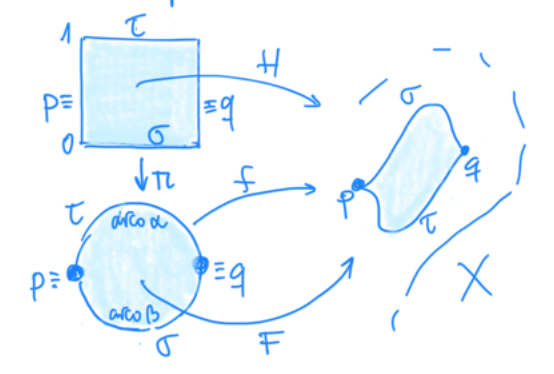
\includegraphics[scale=0.3]{images/def_simple_conx}
    \end{center}
\end{demo}

\begin{ej}
Los conjuntos convexos son simplemente conexos. ¿Los estrellados?
\end{ej}

\section{Esferas \texorpdfstring{$\mathbb{S}^n,\ n \ge 2$}{Sn, n >= 2}}%
\label{sec:esferas_s_n}
\begin{prop}
$\mathbb{S}^n : \{x_1^2 + \ldots + x_{n + 1}^2 = 1\} \subset \mathbb{R}^{n + 1}$ es simplemente conexo ($n \ge 2$).
\end{prop}
\begin{demo}
$\sigma, \tau: \left[ a, b \right] \rightarrow \mathbb{S}^n,\ \sigma\left( a \right) = \tau\left( a \right) = p,\ \sigma\left( b \right) = \tau\left( b \right) = q$.
\[
\exists c, -c \in \mathbb{S}^n\setminus \{p, 1\}\; \land \;\begin{rcases}
   U = \mathbb{S}^n \setminus \{c\} \stackrel{\text{homeo.}}{\approx} \mathbb{R}^n\\
   V = \mathbb{S}^n \setminus \{-c\} \stackrel{\text{homeo.}}{\approx} \mathbb{R}^n
\end{rcases} \text{proyección estéreo.}  
\]
\begin{enumerate}
    \item $\left[ a, b \right] \subset \sigma^{-1}U \cup \sigma^{-1}V \xRightarrow{\text{comp.}} \exists a = t_0 < t_1 < \ldots < t_r = 1: \sigma\left[ t_{i - 1}, t_1 \right] \subset \begin{cases}
        U \text{, ó}\\
        V
    \end{cases}$ dónde $\sigma\left[ t_{i - 1}, t_i \right]$ es la traza de $\sigma_i = \sigma|_{\left[ t_{i - 1}, t_i \right]}$.

    \item Si dos consecutivos están en el mismo $U$ ó $V$, eliminamos la juntura común $\Rightarrow$ al atravesar una juntura $t_k$ cambiamos de $U$ a $V$ ó viceversa, en particular, $x_k = \sigma\left( t_k \right) \in U \cap V \approx \mathbb{R}^n \setminus \{\text{punto}\}$, que es conexo por caminos, o bien, nos quedamos sin junturas y $\sigma\left[ a, b \right] \subset U$ ó $V$.

    \item Consideramos los trozos en $V$ (incluido que $\sigma\left[ a, b \right] \subset V$ porque no hay ya junturas)
    \begin{center}
        \includegraphics[scale=0.3]{images/esferas_sn_3} 
    \end{center}
    \begin{itemize}
        \item[(*)]
        \begin{align*}
            \sigma\left( t_{i - 1} \right), \sigma\left( t_i \right) \in U \cap V &\approx \mathbb{R}^n \setminus \{\text{punto}\} \text{ conexo por caminos}\\
            &\Rightarrow \exists \sigma_i^*: \left[ t_{i - 1}, t_i \right] \rightarrow U\cap V \subset V \text{ mismos extremos que } \sigma_i
        .\end{align*}

        \item[(**)] $V \approx \mathbb{R}^n$ convexo $\Rightarrow \exists H_s^i: \sigma_i \simeq \sigma_i^*$ en $V$ con extremos fijos. ¡Ojo! $\boxed{\sigma_i^*: \left[ t_{i - 1}, t_i \right] \rightarrow U}$.
    \end{itemize}

    \item Pegando a trozos homotopías en $\mathbb{S}^n$:
    \[
    \begin{cases}
        \sigma\left[ t_{i_1}, t_i \right] \subset U \Rightarrow H_s^i \equiv \sigma_i = \sigma_i^*: \left[ t_{i - 1}, t_i \right] \rightarrow U \subset \mathbb{S}^n\\
        \sigma\left[ t_{i_1}, t_i \right] \subset V \xRightarrow{3} H_s^i : \sigma_i \simeq \sigma_i^*: \left[ t_{i - 1}, t_i \right] \rightarrow V \subset \mathbb{S}^n
    \end{cases} \Rightarrow \sigma \simeq \sigma^* 
    \]
    Homótopos en $\mathbb{S}^n$ con extremos fijos, pero $\sigma^*\left[ a, b \right] \subset U$.

    \item Igual, $\exists H_s: \tau \simeq \tau^*$ homotopía en $\mathbb{S}^n$ con extremos fijos, pero $\tau^*\left[ a, b \right] \subset U$.
\end{enumerate}
En conclusión: $\sigma^* \simeq \tau^*$ en $U \left( \approx \mathbb{R}^n \right)$ con extremos fijos $\Rightarrow \sigma \simeq \sigma^* \simeq \tau^* \simeq \tau$ con extremos fijos.
\end{demo}

%\chapter{El grupo fundamental}%
\label{cha:el_grupo_fundamental}
\section{Operaciones con caminos}%
\label{sec:operaciones_con_caminos}
Sea $X$ es conexo por caminos y localmente conexo por caminos.
\begin{defi}[Producto de caminos]
Sean $\sigma, \tau: \left[ 0, 1 \right] \rightarrow X$ tal que $\sigma\left( 1 \right) = \tau\left( 0 \right) \Rightarrow$
\[
\left( \sigma * \tau \right)\left( t \right) = \begin{cases}
    \sigma\left( 2 t \right), &0 \le t \le \frac{1}{2}\\
    \tau\left( 2t - 1 \right), &\frac{1}{2} \le t \le 1
\end{cases}
\]

Que consiste en reescalar $\begin{cases}
    \sigma \text{ de } \left[ 0, 1 \right] \text{ a } \left[ 0, \frac{1}{2} \right]\\
    \tau \text{ de } \left[ 0, 1 \right] \text{ a } \left[ \frac{1}{2}, 1 \right] 
\end{cases}$
\end{defi}

%TODO: Imagen
\begin{center}
    \includegraphics[scale=0.3]{images/prod_grupo_fundamental} 
\end{center}

Las propiedades algebraicas son todas salvo \textit{homotopía con extremos fijos}\footnote{Es decir, la asociatividad, el elemento neutro y el inverso no tienen porque darse en el sentido tradicional de igualdad sino por homotopías.}.
%TODO: Fix
\begin{prop}
\underline{Propiedades} de grupo:
\begin{enumerate}
    \item \underline{Asociativa}: $\left( \alpha * \beta \right) * \gamma \simeq \alpha * \left( \beta * \gamma \right)$.

    En cada altura $s$ se reescalan los caminos con junturas.
    \begin{center}
        \includegraphics[scale=0.3]{images/asoc_gr_fund} 
    \end{center}
    \item \underline{Neutro}: 
    \begin{center}
        \includegraphics[scale=0.3]{images/neutro_gr_fund} 
    \end{center}
    \item \underline{Inverso}: $\sigma'\left( t \right) = \sigma\left( 1 - t \right) \Rightarrow \sigma * \sigma' \simeq e_0$ y $\sigma'' = \sigma \Rightarrow \sigma' * \sigma \simeq e_1$.

    No se reescala: $0 \le \frac{1 - s}{2} \le \frac{1 + s}{2} \le 1$. 

    Las junturas dicen dónde parar $\sigma$ y empezar $\sigma'$ en cada altura:
    \begin{center}
        \includegraphics[scale=0.3]{images/inv_gr_fund} 
    \end{center}

    \item \underline{Invarianza por homotopía}: 
    \begin{gather*}
        \begin{cases}
            F_s: \sigma_1 \simeq \sigma_2\\
            G_s: \tau_1 \simeq \tau_2
        \end{cases} \xRightarrow{\text{Trans.}} F_s * G_s: \sigma_1 * \tau_1 \simeq \sigma_2 * \tau_2\\
        F_s * G_s\left( t \right) = \begin{cases}
            F_s\left( 2t \right),\ 0 \le t \le \frac{1}{2},\\
            G_s\left( 2t - 1 \right),\ \frac{1}{2} \le t \le 1
        \end{cases} 
    .\end{gather*}

\end{enumerate}
\end{prop}

\section{El grupo fundamental}%
\label{sec:el_grupo_fundamental}
Sea $X$ conexo por caminos, $x_0 \in X$ \underline{punto base} fijo.
\begin{defi}
\begin{enumerate}
    \item \textbf{Lazo de base $x_0$}:
    \[
        \sigma: \left[ 0, 1 \right] \rightarrow X,\ \underbrace{\sigma\left( 0 \right) = \sigma\left( 1 \right)}_{\text{lazo}} = x_0 \text{, punto fijo.}
    \]

    \item Sean $\sigma, \tau: \left[ 0, 1 \right] \rightarrow X$ lazos de base $x_0$:
    \begin{itemize}
        \item \textbf{Homotopía de lazos}: $H_s: \sigma \simeq \tau$ tal que $H_s\left( 0 \right) = H_s\left( 1 \right),\ \forall s$.
        \item \textbf{Homotopía de lazos con punto base fijo}: $H_s = \sigma \stackrel{x_0}{\simeq} \tau$ tal que $H_s\left( 0 \right) = H_s\left( 1 \right) = x_0,\ \forall s$. (Relativa a $\{0, 1\}$)
    \end{itemize}
\end{enumerate}
\end{defi}
\begin{defi}[Grupo fundamental]
\begin{itemize}
    Llamamos \textbf{grupo fundamental de $X$ con base $x_0$} a:
    \[
    \boxed{\pi\left( X, x_0 \right) = \faktor{\left\{ \text{lazos de base } x_0 \right\}}{\stackrel[x_0]{}{\simeq}}}
    \] (``Lazos'' / ``Homotopía")

\end{itemize}
\end{defi}

\begin{obs}
$\left[ \sigma \right] * \left[ \tau \right] = \left[ \sigma * \tau \right]$ define bien un grupo por \ref{sec:operaciones_con_caminos}.
\end{obs}

\begin{ej}
\begin{enumerate}
    \item $X$ simplemente conexo $\Leftrightarrow \pi\left( X, x_0 \right) = \{1\},\ \forall x_0$. [$\Leftarrow)$ ejercicio]
    \item $\pi\left( \mathbb{S}^n, x_0 \right) = \{1\},\ n \ge 2$.
    \begin{demo}
    Por $1)$ y ser $\mathbb{S^n},\ n \ge 2$ simplemente conexa.
    \end{demo}
    \item $\pi\left( \mathbb{R}\mathrm{P}^n, x_0 \right) = \mathbb{Z}_2,\ n \ge 2$.
    \item $\pi\left( \mathbb{S}^1, x_0 \right) = \mathbb{Z},\ \pi\left( \text{banda Möbius} \right) = \mathbb{Z}$.
    \item $\pi\left( \infty, x_0 \right) = \mathbb{Z} * \mathbb{Z}$ que es una lemniscata y un \textbf{grupo libre} \underline{no conmutativo}.
\end{enumerate}
\end{ej}
El cálculo de grupos fundamentales no es una tarea trivial, pero muy útil.

El punto base no es muy importante.
\begin{prop}[Isomorfismo por punto base]
Sea $\alpha: \left[ 0, 1 \right] \rightarrow X$ de $\alpha\left( 0 \right) = x_0$ a $\alpha\left( 1 \right) = x_1$. La \textbf{conjugación por $\alpha$}:
\begin{align*}
    \pi\left( X, x_0 \right) &\rightarrow \pi\left( X, x_1 \right)\\
    \left[ \sigma \right] &\mapsto \left[ \alpha' * \sigma * \alpha \right] 
.\end{align*}
es isomorfismo de grupos (por homotopía).
%TODO: Imagen
\begin{center}
    \includegraphics[scale=0.3]{images/conj_iso_grupos} 
\end{center}
\end{prop}
\begin{demo}
Fácil con las propiedades de \ref{sec:operaciones_con_caminos}.
\end{demo}

\section{Funtorialidad}%
\label{sec:funtorialidad}
\begin{defi}    
Definimos $h_*$ como:
\begin{align*}
    h: X \rightarrow Y &\text{ homeo, } h\left( x_0 \right) = y_0 \Rightarrow\\
    h_*: \pi\left( X, x_0 \right) &\rightarrow \pi\left( Y, y_0 \right) \text{ iso.}\\
    \left[ \sigma \right] &\mapsto \left[ h \circ \sigma \right] 
.\end{align*}
\end{defi}
Es fácil y útil: espacios homeomorfos deben tener grupos fundamentales isomorfos.

Por ejemplo, $\mathbb{S}^2$ y $\mathbb{R}P^2$ no son homeomorfos. Pero la construcción es mucho más general.
%TODO: Imagen
\begin{center}
    \includegraphics[scale=0.3]{images/const_functorialidad} 
\end{center}

\begin{defi}[Funtorialidad]
$\left( g \circ f \right)_* = g_* \circ f_*$ y $\left( id_X \right)_* = id_{\pi\left( X, x_0 \right)}$. 
\end{defi}

\begin{ej}
    Si $h: X \rightarrow Y,\ x_0 \mapsto y_0$ es homeomorfismo $\Rightarrow \left( h_* \right)^{-1} = \left( h^{-1} \right)_*$. [Más preciso que $h_*$ isomorfismo]
\end{ej}

\begin{prop}[Producto de espacios]
Tenemos que si:
%TODO: Imagen
\begin{center}
    \includegraphics[scale=0.3]{images/prod_espacios_funt} 
\end{center} 
entonces:
\begin{align*}
    \pi\left( X \times Y, \left( x_0, y_0 \right) \right) &\xrightarrow{p_*, q_*} \pi\left( X, x_0 \right) \times \pi \left( Y, y_0 \right)\\
    \left[ \gamma \right] = \left[ \left( \sigma; \tau \right) \right] &\mapsto \left( \left[ \sigma \right], \left[ \tau \right] \right)
.\end{align*}
es un isomorfismo.
\end{prop}
\begin{demo}
Sean:
\[
\begin{rcases}
    F_s: \sigma_1 \stackrel{x_0}{\simeq} \sigma_2\\
    G_s: \tau_1 \stackrel{y_0}{\simeq} \tau_2
\end{rcases} \Rightarrow \left( F_s, G_s \right): \left( \sigma_1, \tau_1 \right) = \gamma_1 \mapsto \gamma_2 = \left( \sigma_2, \tau_2 \right) \text{ y nada más...} 
\]
\end{demo}

\begin{ej}
\begin{enumerate}
    \item $\pi\left( \mathbb{S} \times \mathbb{S} \right) = \pi\left( \mathbb{S} \right) \times \pi\left( \mathbb{S} \right) = \mathbb{Z}^2$.
    \item $\pi\left( \mathbb{S}^1 \times \left[ 0, 1 \right] \right) = \pi\left( \mathbb{S} \right) \times \pi\left( \left[ 0, 1 \right] \right)$.
\end{enumerate}
\end{ej}

%\chapter{Retractos}%
\label{cha:retractos}
\section{Retractos y deformaciones}%
\label{sec:retractos_y_deformaciones}
\begin{defi}
Una aplicación $\rho: X \rightarrow A \subset X$ es:
\begin{enumerate}
    \item Un \textbf{retracto} si $\rho|_A = id_A$ (y $A = \rho\left( A \right)$ es un \underline{retracto de $X$})
    \item Una \textbf{deformación} (fuerte) si: $\exists H_s: id_X \stackrel{A}{\simeq} \rho$, homotopía relativa a $A$.
\end{enumerate}
\end{defi}

\begin{ej}
\begin{enumerate}
    \item $\forall$ cte $: X \rightarrow \{x_0\} \subset X$ es retracto.
    \item El retracto \underline{radial} $\rho: \mathbb{R}^{n + 1} \setminus \{0\} \rightarrow \mathbb{S}^n: x \mapsto x / \lVert x \rVert$ es una deformación. $H_s\left( x \right) = \left( 1 - s \right) x + s\rho\left( x \right)$.
    \item $\begin{rcases}
        \rho: X \rightarrow A \subset X \subset \mathbb{R}^n \text{ retracto}\\
        \left[ x, \rho\left( x \right) \right] \subset X,\ \forall x
    \end{rcases} \Rightarrow \rho$ deformación: $H_s = \left( 1 - s \right) id_X + s\rho$ (interpolación).
    \item Cilindros: 
    \begin{align*}
        \rho: X \times \left[ 0, 1 \right] &\rightarrow X \times \{0\}\\
        \left( x, t \right) &\mapsto \left( x, 0 \right) = \rho \left( x, t \right) 
    .\end{align*}
    con $\rho$ deformación sobre $X : H_s\left( x, t \right) = \left( x, \underbrace{\left( 1 - s \right) t}_{\left( 1 - s \right) t + s \cdot 0} \right)$.
    %TODO: Imagen
    \begin{center}
        \includegraphics[scale=0.3]{images/deformacion_cilindros} 
    \end{center}
    \item Banda de Möbius: $\mathbb{S}^1 \subset M = \bigcup_{p \in \mathbb{S}^1} \left[ a_p, b_p \right]$.

    Deformación sobre $\mathbb{S}^1: \begin{cases}
        \rho: M \rightarrow \mathbb{S}^1: x \mapsto \rho\left( x \right)\\
        H_s\left( x, s \right) = \left( 1 - s \right) x + s\rho\left( x \right) 
    \end{cases}$
    %TODO: Imagen
    \begin{center}
        \includegraphics[scale=0.3]{images/deformacion_moebius} 
    \end{center}
\end{enumerate}
\end{ej}

\begin{prop}
Sea $\rho: X \rightarrow A \subset X,\ a_0 \in A;\ \rho_*: \pi\left( X, a_0 \right) \rightarrow \pi\left( A, a_0 \right)$.
\begin{enumerate}
    \item $\rho$ retracto $\Rightarrow \rho_*$ suprayectivo.
    \item $\rho$ deformación $\Rightarrow \rho_*$ isomorfismo.
\end{enumerate}
\end{prop}
\begin{demo}
\begin{enumerate}
    \item $\rho$ retracto:
    %TODO: Imagen
    \begin{center}
        \includegraphics[scale=0.3]{images/dem_retracto_sobre} 
    \end{center}

    \item $\rho$ deformación:
    \[
    H_s: id_X \stackrel{A}{\simeq} \rho \Rightarrow j_* \text{ sobre.} : \begin{cases}
        \left[ \sigma \right] \in \pi\left( X, a_0 \right) &\Rightarrow H_s \circ \sigma: \sigma \stackrel{A}{\simeq} \rho \circ \sigma = j \circ \rho \circ \sigma\\
           &\Rightarrow \left[ \sigma \right] = \left[ j \circ \rho \circ \sigma \right] = j_*\left[ \rho \circ \sigma \right] 
    \end{cases} 
    \]
    y por ser $j_*$ sobre $\Rightarrow \rho_*$ inyectiva.
\end{enumerate}
\end{demo}

\begin{ej}
\begin{enumerate}
    \item $\pi\left( \mathbb{R}^{n + 1?} \setminus \{0\} \right) = \pi\left( \mathbb{S}^n \right) = \begin{cases}
        \{1\},\ n\ge 2\\
        \mathbb{Z},\ n = 1
    \end{cases}$
    \item $\pi$(cilindro) = $\pi$(banda de Möbius) $= \pi \left( \mathbb{S}^1 \right) = \mathbb{Z}$.
\end{enumerate}
\begin{demo}
    Veremos $\mathbb{S}^1$...
\end{demo}
\end{ej}

\section{Cocientes}%
\label{sec:cocientes}
Muchos espacios son cocientes y las deformaciones se pueden hacer compatibles para facilitar las construcciones.

\begin{ej}
Cilindro $C = \mathbb{S}^1 \times \left[ 0, 1 \right]$ y banda de Möbius $M$.
%TODO: Imagen
\begin{center}
    \includegraphics[scale=0.3]{images/coc_cilindro_moebius} 
\end{center}
Tenemos $C, M = R / $ identificaciones adecuadas de lados opuestos y, por otro lado, la deformación de $R$ sobre $A = \left[ a, b \right],\ H_s\left( z \right) = \left( 1 - s \right) z + s \rho\left( z \right) \xRightarrow{(*)}$ deformación de $R / \sim$ sobre $\left[ a, b \right] / \sim = \mathbb{S}^1$. 

Es decir, \fbox{$\mathbb{S}^1$ es deformación de $C$ y de $M$, luego todos tienen $\pi = \mathbb{Z}$.} 

$(*)$: porque $p$ y $H_s$ son \underline{compatibles con las relaciones}: $z \sim z' \Rightarrow H_s\left( z \right) \simeq H_s\left( z' \right)$, luego inducen aplicaciones continuas $\overline{\rho}$ y $\overline{H_s}: R / \sim\ \rightarrow A / \sim$. 

Normalmente se hacen las deformaciones pensando en que cumplan $H_s\left( z \right) \simeq H_s\left( z' \right)$.
\end{ej}

\section{Agujeros}%
\label{sec:agujeros}
Conviene insistir en un ejemplo importante de deformación y sus variantes.
%TODO: No sé que entorno usar aquí
\begin{enumerate}
    \item $\rho: \underbrace{\mathbb{R}^{n + 1} \setminus \{0\}}_{\text{esp. con ``agujero''}}  \rightarrow \mathbb{S}^n$ deformación $\Rightarrow \pi\left( \mathbb{R}^{n + 1} \setminus \{0\}, x_0 \right) =$ \[
    = \begin{cases}
        \mathbb{Z},\ n = 1 \text{ (se verá...)}\\
        \{1\},\ n \ge 2\ (\mathbb{S}^n,\ n \ge 2 \text{ simple-conexa}) 
    \end{cases} 
    \]

    \item Dibujos en $\mathbb{R}^2 \setminus \{c\}$ de retracciones sobre curvas ``alrededor'' del ``agujero'' $c$:
    %TODO: Imagen
    \begin{center}
        \includegraphics[scale=0.3]{images/curvas_R2_agujero_c} 
    \end{center}

    \item Dos agujeros $\mathbb{R}^2 \setminus \{a, b\}$.

    Se trocea el espacio en cerrados, en cada uno de los cuáles se hace una deformación, de manera que en las fronteras coincidan. En el dibujo se sombrean diferentes las zonas en las que se usan deformaciones diferentes. Las deformaciones más cómodas son las interpolaciones de $id$ y una retracción geométrica.
    %TODO: Imagen
    \begin{center}
        \includegraphics[scale=0.3]{images/curvas_R2_dos_agujeros} 
    \end{center}
    En este caso, $\rho: \mathbb{R}^2 \setminus \{a, b\} \rightarrow \infty?$ es deformación y $\pi\left( \mathbb{R}^2 \setminus \{a, b\}, x_0 \right) = \pi\left( \infty? \right) = \mathbb{Z} * \mathbb{Z}$ (grupo fundamental de una lemniscata).

    \item Otra variante:
    %TODO: Imagen
    \begin{center}
        \includegraphics[scale=0.3]{images/variante_4_agujeros} 
    \end{center}
    %TODO
    $\mathbb{R}^2 \setminus \{a, b\} \rightarrow dibujo$ deformación dice que:
    \[
    \pi\left( dibujo \right) = \pi\left( \mathbb{R}^2 \setminus \{a, b\}, x_0 \right) = \pi \underbrace{\left( \infty? \right)}_{= \mathbb{Z} * \mathbb{Z}}  
    \]
    que es igual al grupo fundamental, pero \underline{no} homeomorfismo.

    \item Aún más ejemplos así (ya sin especificar el punto base):
    \[
    \pi\left( \mathbb{R}^2 \setminus \{a, b, c\} \right) = \pi\left( dibujo \right) = \pi\left( dibujo \right) = \pi \left( dibujo \right) = \mathbb{Z} * \mathbb{Z} * \mathbb{Z}
    \]
    \begin{demo}[creo]
    Cualesquiera tres puntos en $\mathbb{R}^2$ se pueden recolocar con homeomorfismos para hacer, a partir de ellos, retracciones sobre las curvas dibujadas, \underline{no homeomorfas}. (?) 
    \end{demo}
\end{enumerate}

\underline{Ejercicio}: Deformar $\mathbb{R}\mathrm{P}^2 \setminus \{a\}$ sobre una circunferencia, para obtener $\pi\left( \mathbb{R}\mathrm{P}^2 \setminus \{a\} \right) = \mathbb{Z}$.


%\chapter{Recubridores}%
\label{cha:recubridores}
\section{El problema de elevación}%
\label{sec:el_problema_de_elevacion}
Fijada $p$, qué $f$'s tienen \underline{elevación} $\tilde{f}$. i.e: $p \circ \tilde{f} = f$ 
%TODO: Imagen
\begin{center}
    \includegraphics[scale=0.3]{images/problema_elevacion} 
\end{center}
\begin{defi}
$p$ es un \textbf{recubridor} si $\forall x \in X,\ \exists U^x \text{, abierto \textbf{trivializante}} : p^{-1}\left( U^x \right) = \bigsqcup_{\lambda} U_{\lambda}$ y $\forall \lambda, p|: U_{\lambda} \rightarrow U^x$ homeomorfismo.
\end{defi}
Es un tipo especial de homeomorfismo local sobreyectivo y, por eso, identificación abierta.

\begin{ej}[¡Importantes!]
\begin{enumerate}
    \item La identificación \underline{antipodal}, $\pi: \mathbb{S} \rightarrow \mathbb{R}\mathrm{P}^n$,
    \[
    \forall x \in \mathbb{R}\mathrm{P}^n \underbrace{\exists U^x}_{\text{trivializante}} = \mathbb{R}\mathrm{P}^n \setminus \underbrace{H}_{\text{hiperplano}}\; \land \;\pi^{-1}\left( U^x \right) = \mathbb{S}^n\setminus \pi^{-1}H = S_+ \sqcup S_-  
    \]
    hemisferios abiertos.

    Ya se ilustró convenientemente en su lección. ¿Qué se tiene para $n = 1$?

    \item La identificación \underline{exponencial}, $p: \mathbb{R} \rightarrow \mathbb{S}^1: \theta \mapsto e^{2ni\theta} = \left( \cos 2\pi\theta, \sin 2\pi\theta \right)$.
    %TODO: Imagen
    \begin{center}
        \includegraphics[scale=0.2]{images/identificacion_exponencial} 
    \end{center}
\end{enumerate} 
\end{ej}

\section{Unicidad de elevación}%
\label{sec:unicidad_de_elevacion}
\begin{prop}
Si $Z$ es conexo, dos elevaciones que coinciden en algún puntos son iguales.
\end{prop}
\begin{demo}
    $A = \{z \in Z: \tilde{f}_1 \left( z \right) = \tilde{f}_2\left( z \right)\}, p \circ \tilde{f}_1 = f$.
    \begin{align*}
        \underbrace{x}_{f\left( z \right)} \in U^x,\ p^{-1} U^x &= \bigsqcup_{\lambda} U_{\lambda} \text{ (trivialización)} \Rightarrow \tilde{f}_i\left( z \right) \in p ^{-1}U^x\; \land \;\exists!\lambda_i: \tilde{f}_i\left( z \right) \in U_{\lambda_i}\\
        &\Rightarrow \forall \xi \in W^z = \tilde{f}_1^{-1}\left( U_{\lambda_1} \right) \cap \tilde{f}_2^{-1} \left( U_{\lambda_2} \right): \hat{f}_1\left( \xi \right) = \hat{f}_2\left( \xi \right) \stackrel{(*)}{\Leftrightarrow} \lambda_1 = \lambda_2 (**)
    .\end{align*}
    $(*)$ debido a: 
    \begin{itemize}
        \item $\Rightarrow) U_{\lambda}$'s disjuntos. 
        \item $\Leftarrow) p \tilde{f}_1 = p \tilde{f}_2$ y $p|_{U_\lambda}$ 1-1.
    \end{itemize}

    Por tanto, 
    \begin{itemize}
        \item \underline{Abierto}:
        \begin{align*}
            W^z \subset A \text{ si } z \in A: \tilde{f}_1\left( z \right) = \tilde{f}_2\left( z \right) &\stackrel{(**)}{\Rightarrow} \lambda_1 = \lambda_2 \Rightarrow \tilde{f}_1\left( W^z \right)\ \land \ \tilde{f}_2\left( W^z \right) \subset U_{\lambda_1} = U_{\lambda_2} \xrightarrow{p|} \underbrace{U^x }_{\text{iny.}}\\
            &\Rightarrow \forall \xi \in W^z: \tilde{f}_1\left( \xi \right),\ \tilde{f}_2\left( \xi \right) \mapsto f\left( z \right) \Rightarrow \tilde{f}_1\left( \xi \right) = \tilde{f}_2\left( \xi \right)
        .\end{align*}

        \item \underline{Cerrado}:
        \begin{align*}
            W^z \subset Z \setminus A \text{ si } z \not\in A: \tilde{f}_1\left( z \right) \neq \tilde{f}_2\left( z \right) &\stackrel{(**)}{\Rightarrow} \lambda_1 \neq \lambda_2 \Rightarrow \tilde{f}_1\left( W^z \right) \cap \tilde{f}_2\left( W^z \right) \subset U_{\lambda_1} \cap U_{\lambda_2} = \emptyset\\
            &\Rightarrow \forall \xi \in W^z: \tilde{f}_1\left( \xi \right) \neq \tilde{f}_2\left( \xi \right) 
        .\end{align*}
    \end{itemize}
    Por tanto, 
    \[
        \exists \tilde{f}_1\left( z \right) = \tilde{f}_2\left( z \right) \Rightarrow \emptyset \neq A \stackrel[\text{cerr.}]{\text{ab.}}{\subset} Z \text{ conx.} \Rightarrow A = Z\; \land \;\tilde{f}_1 = \tilde{f}_2
    \]
\end{demo}

\section{Lema de elevación}%
\label{sec:lema_de_elevaccion}
\begin{prop}
Tenemos que:
\[
\begin{cases}
    f = H: Y \times \left[ 0, 1 \right] \rightarrow X \text{ (homotopía)} \\
    \exists \tilde{H}_0 \text{ elevación de } H_0: Y \rightarrow X
\end{cases} \Rightarrow \exists \tilde{H} \text{ elevación, } \left( \tilde{H} \right)_0 = \tilde{H}_0
\]
\end{prop}
\begin{demo}
\begin{enumerate}
    \item \underline{Elevación semilocal}: $\forall y \in Y,\ \tilde{H}^y: V^y \times \left[ 0, 1 \right] \rightarrow \tilde{X}$ elevación de $H|_{V^y \times \left[ 0, 1 \right]}$.
    \begin{enumerate}
        \item $\{y\} \times \left[ 0, 1 \right] \subset \bigcup_{x} H^{-1}\left( U^x \right),\ p ^{-1} U^x = \bigsqcup_{\lambda} U_{\lambda}$ (trivialización en $x$) $\Rightarrow$
        \begin{align*}
            &\xRightarrow{\text{comp.}} \exists 0 = t_0 < t_1 < \ldots < t_r = 1: \{y\} \times \left[ t_{i - 1}, t_i \right] \subset H^{-1}\left( U^{x_i} \right)\\
            &\xRightarrow{\text{comp.}} \forall i,\ \exists V_i^y \times \left[ t_{i-1}, t_i \right] \subset H^{-1}\left( U^{x_i} \right)\\
            &\Rightarrow \exists V^y = V_1^y \cap \ldots \cap V_r^y: V^y \times \left[ t_{i - 1}, t_i \right] \stackrel{(*)}{\subset} H^{-1}\left( U^{x_i} \right)
        .\end{align*}

        \item Inducción, $i > 0: \exists \tilde{H}_0: V^y \times \{t_0\} \rightarrow \tilde{X}$ por hipótesis. 
        \begin{align*}
            \underline{i - 1 \rightarrow i}:\ &\exists H_{i - 1}^y \text{ en } V^y \times \left[ t_0, t_{i - 1?} \right] \Rightarrow \text{se puede extender a } V^y \times \left[ t_{i - 1}, t_i \right] \\
            (*) &\Rightarrow \begin{cases}
                H\left( y, t_{i - 1} \right) \in U^{x_i} \xRightarrow{\exists \lambda} \tilde{H}_{i - 1}^y \left( y, t_{i - 1} \right) \in U_{\lambda} \xRightarrow{\text{red. } V^y}\\
                \qquad \hat{H}_{i - 1}^y \left( V^y \times \left( t_{i - 1} \right) \right) \subset U_{\lambda} \rightarrow U^{x_i}\\
                \exists \left( p|_{U_{\lambda}}^{-1}\right) \circ H: V^y \times \left[ t_{i - 1}, t_i \right] \rightarrow U_{\lambda} \text{ elevación (de } H)
            \end{cases}\\
                &\Rightarrow p\circ\tilde{H}_{i - 1}^y = p \circ \left[ \left( p|_{U_{\lambda}}^{-1} \circ H \right) \right]: V^y \times \{t_{i - 1}\} \rightarrow U^{x_i}\\
                &\quad \xRightarrow{p|_{U_\lambda} \text{ iny.}} \tilde{H}_{i - 1}^y = \left( p|_{U_{\lambda}} \right)^{-1} \circ H \text{ en } V^y \times \{t_{i - 1}\}\\
                &\Rightarrow \left( p|_{U_{\lambda}}^{-1} \right) \circ H \text{ extiende } \tilde{H}_{i - 1}^y \text{ a } V^y \times \left[ t_{i - 1}, t_i \right] 
        .\end{align*}
    \end{enumerate}

    \item \underline{Elevación global}. Las locales $\{\tilde{H}^y: V^y \times \left[ 0, 1 \right] \rightarrow \tilde{X}\}_{y \in Y}$ encolan bien, pues coinciden en las intersecciones: $\forall y \in V^{y_1} \cap V^{y_2}$:
\end{enumerate}
\end{demo}

\begin{obs}
\begin{enumerate}
    \item La elevación de una aplicación $Y \rightarrow X$ sólo depende de su clase de homotopía.
    \item Todo camino $\sigma: \left[ 0, 1 \right] \rightarrow X$ tiene uan única elevación $\tilde{\sigma}$ con origen $\tilde{\sigma}\left( 0 \right) \in p^{-1}\left( \sigma\left( 0 \right) \right)$.
    \[
    \begin{rcases}
    \begin{rcases}
        \tilde{H}^{y_1} \left( y, \bullet \right)\\
        \tilde{H}^{y_2} \left( y, \bullet \right) 
    \end{rcases} \text{elevan } H\left( y, \bullet \right) : \{y\} \times \left[ 0, 1 \right] \\  
    \tilde{H}^{y_1} \left( y, 0 \right) = \tilde{H}_0\left( y \right) = \tilde{H}^{y_2} \left( y, 0 \right) \text{ 1\textsuperscript{er} paso ind.} 
    \end{rcases} \xRightarrow{\text{Uni. elevaccón.}} 
    \tilde{H}^{y_1} \left( y, t \right) = \tilde{H}^{y_2} \left( y, t \right),\ \forall z
    \]
\end{enumerate}
\end{obs}


\chapter{Cálculos mediante recubridores}%
\label{cha:calculos_mediante_recubridores}
Hemos visto ya que:
\begin{itemize}
    \item $\pi$(estrellado) $= \{1\},\ \pi\left( \mathbb{S}^n \right) = \{1\},\ n \ge 2 \Rightarrow \pi\left( \mathbb{R}^{n + 1} \setminus \{0\} \right) = \{1\}$.
    \item $\pi\left( \mathbb{P}^{n} \right) = \mathbb{Z}_2,\ n \ge  2$ (no demostrado)
    \item $\pi\left( \mathbb{S}^1 \right) = \mathbb{Z}$ (no demostrado).
    \begin{itemize}
        \item $\pi$(toro) $= \mathbb{Z} \times \mathbb{Z},\ \pi$(cilindro) $= \mathbb{Z}$.
        \item $\pi$(banda de Möbius) $= \mathbb{Z},\ \pi\left( \mathbb{R}^2 \setminus \{a\} \right) = \mathbb{Z}$.
    \end{itemize}
    Ahora toca demostrar $\pi\left( \mathbb{P}^{n} \right)$ y $\pi\left( \mathbb{S}^1 \right)$.
\end{itemize}

\section{Espacios proyectivos reales}%
\label{sec:espacios_proyectivos_reales_rec}
\begin{theo}
$\pi\left( \mathbb{P}^{n} \right) = \mathbb{Z}_2,\ n \ge 2$
\end{theo}
\begin{demo}
Usamos el recubridor antipodal $p : \mathbb{S}^n \rightarrow \mathbb{P}^{n}: \tilde{x}, -\tilde{x} \mapsto x = \left[ \tilde{x} \right] = \left[ - \tilde{x} \right]$. Punto base en $\mathbb{P}^{n}: x_0 = \left( 0 : \ldots : 1 \right);\ \sigma: \left[ 0, 1 \right] \rightarrow \mathbb{P}^{n},\ \sigma\left( 0 \right) = \sigma\left( 1 \right) = x_0,\ \tilde{x}_0 = \left( 0, \ldots, 1 \right)$. Ahora, por el lema de elevación:
\[
    \Rightarrow \exists! \tilde{\sigma}: \left[ 0, 1 \right] \rightarrow \mathbb{S}^{n},\ p\tilde{\sigma} = \sigma,\ \tilde{\sigma} = \tilde{x}_0\; \land \;\tilde{\sigma}\left( 1 \right) \in p^{-1}\left( x_0 \right) = \{\tilde{x}_0, -\tilde{x}_0\}  
\]
No veces? lazo.
\begin{enumerate}
    \item $\tilde{\sigma}\left( 1 \right) = \tilde{x}_0 \xRightarrow{\mathbb{S}^{n} \text{ simple conx.}} \exists \tilde{H}_s: \tilde{\sigma} \stackrel{x_0}{\simeq} \tilde{x}_0 \Rightarrow \exists p \circ \tilde{H}_s: \sigma \stackrel{x_0}{\simeq} x_0 \Rightarrow \left[ \sigma \right] = 1 \in \pi\left( \mathbb{P}^{n}, x_0 \right)$. 

    \item $\tilde{\sigma} \left( 1 \right) = -\tilde{x}_0 \xRightarrow{\mathbb{S}^{n} \text{ simple conx.}} \exists \tilde{H}_s: \tilde{\sigma} \stackrel{\tilde{x}_0,-\tilde{x}_0}{\simeq} \tilde{\alpha} = \left( 0, \ldots, 0, \sin \pi t, \cos \pi t \right) \Rightarrow \exists p \circ H_s: \sigma \stackrel{x_0}{\simeq} \alpha = p \circ \tilde{\alpha}$, lazo de base $x_0,\ \alpha\left( 0 \right) = \alpha\left( 1 \right) = x_0$. 

    \item Tenemos:
    %TODO: Imagen
    \begin{center}
        \includegraphics[scale=0.3]{images/rec_esp_proy_r} 
    \end{center}

    \item[1. 2. 3.] $\Rightarrow \pi\left( \mathbb{P}^{n}, x_0 \right)$ tiene dos elementos distintos dependiendo del extremo de la elevación $\Rightarrow$ 
        \[
        \boxed{\pi\left( \mathbb{P}^{n}, x_0 \right) = \mathbb{Z}_2}.
        \]
\end{enumerate}
\end{demo}

\section{La circunferencia}%
\label{sec:la_circunferencia}
\begin{theo}
$\pi\left( \mathbb{S}^{1} \right) = \mathbb{Z}$.
\end{theo}
\begin{obs}
$\mathbb{S}^{1} = \mathbb{P}^{1}$.
\end{obs}
\begin{demo}
    Usamos el recubridor exponencial $p: \mathbb{R} \rightarrow \mathbb{S}^{1}: \theta \mapsto \left( \cos 2 \pi \theta, \sin 2 \pi \theta \right)$. Punto base $x_0 \in \mathbb{S}^{1},\ \forall \sigma: \left[ 0, 1 \right] \rightarrow \mathbb{S}^{1},\ s\left( 0 \right) = \sigma\left( 1 \right) = x_0$. Por el lema de elevación:
    \[
    \Rightarrow \exists \tilde{\sigma} : \left[ 0, 1 \right] \rightarrow \mathbb{R}^{}, p \tilde{\sigma} = \sigma \Rightarrow p \tilde{\sigma} \left( 1 \right) = \sigma\left( 1 \right) = \sigma\left( 0 \right) = p \tilde{\sigma} \left( 0 \right) \Rightarrow \tilde{\sigma} \left( 1 \right) = \tilde{\sigma} \left( 0 \right) + k,\ k \in \mathbb{Z}
    \]

\begin{theo}
    El \underline{nº de vueltas}:
    \begin{align*}
        \#: \pi\left( \mathbb{S}^{1}, x_0 \right) &\rightarrow \mathbb{Z}\\
        \left[ \sigma \right] &\mapsto \# \sigma = \tilde{\sigma}\left( 1 \right) - \tilde{\sigma}\left( 0 \right) 
    .\end{align*}
    es isomorfismo de grupos bien definido.
\end{theo}
\begin{demo}
    \begin{enumerate}
        \item $k = \tilde{\sigma} \left( 1 \right) - \tilde{\sigma} \left( 0 \right)$ no depende de $\tilde{\sigma}$. 
        \begin{align*}
            p \tilde{\tau} = \sigma = p \tilde{\sigma} &\Rightarrow \tilde{\tau} \left( 0 \right) = \tilde{\sigma} \left( 0 \right) + l \Rightarrow \begin{cases}
                \tilde{\tau}\\
                \tilde{\sigma} + l
            \end{cases} \parbox{5em}{elevan $\sigma$\\ coinciden\\ en $t = 0$} \xRightarrow{\text{uni. elev.}} \tilde{\tau} = \tilde{\sigma} + l\\
            &\Rightarrow k = \tilde{\sigma}\left( 1 \right) - \tilde{\sigma} \left( 0 \right) = \left( \tilde{\tau} \left( 1 \right) - l \right) - \left( \tilde{\tau} \left( 0 \right) - l \right) = \tilde{\tau} \left( 1 \right) - \tilde{\tau} \left( 0 \right) 
        .\end{align*}

        \item $k$ no depende de homotopía de lazos, luego $\#$ está bien definido. Sea $H_s: \sigma \simeq \tau$ y $H_s\left( 1 \right) = H_s\left( 0 \right),\ \forall s$:
        \begin{align*}
            &\Rightarrow \exists \tilde{H}_s: \tilde{\sigma} \simeq \tilde{\tau} \text{ entre elevaciones de } \sigma\; \land \;\tau\\
            &\Rightarrow s \mapsto \underbrace{\tilde{H}_s\left( 1 \right)}_{\xrightarrow{p} H_s\left( 1 \right) }  \setminus \underbrace{\tilde{H}_s\left( 0 \right)}_{\xrightarrow{p} H_s\left( 0 \right)} \in \mathbb{Z} \xRightarrow{\text{cont.}} \tilde{H}_s\left( 1 \right) - \tilde{H}_s\left( 0 \right) \equiv cte.\\
            &\Rightarrow k = \tilde{\sigma} \left( 1 \right) - \tilde{\sigma} \left( 0 \right) = \tilde{H}_0\left( 1 \right) - \tilde{H}_0\left( 0 \right) \stackrel{cte.}{=} \tilde{H}_1\left( 1 \right) - \tilde{H}_1\left( 0 \right) = \tilde{\tau} \left( 1 \right) - \tilde{\tau} \left( 0 \right)  
        .\end{align*}

        \item $\#$ es isomorfismo. Sea $\# \sigma = \tilde{\sigma} \left( 1 \right) - \tilde{\sigma} \left( 0 \right)$ y $\# \tau = \tilde{\tau} \left( 1 \right) - \tilde{\tau} \left( 0 \right)$ y:
        \begin{align*}
            \tau\left( 0 \right) = \tau\left( 1 \right) = p \tilde{\sigma} \left( 1 \right) &\Rightarrow \tilde{\sigma} \left( 1 \right) \text{ cond. inicial elev.} \\
            &\Rightarrow \exists \tilde{\tau} : \underline{\tilde{\tau} \left( 0 \right) = \tilde{\sigma} \left( 1 \right)} \Rightarrow \tilde{\sigma} * \tilde{\tau} = \tilde{\sigma * \tau} 
        .\end{align*}
        Entonces:
        \begin{align*}
            \# \left( \sigma * \tau \right) &= \tilde{\sigma * \tau} \left( 1 \right) - \tilde{\sigma * \tau} \left( 0 \right) = \tilde{\sigma} * \tilde{\tau} \left( 1 \right) - \tilde{\sigma} * \tilde{\tau} \left( 0 \right) = \tilde{\tau} \left( 1 \right) - \tilde{\sigma} \left( 0 \right) =\\
            &= \left( \tilde{\tau} \left( 1 \right) - \tilde{\tau} \left( 0 \right) \right) + \left( \tilde{\sigma} \left( 1 \right) - \tilde{\sigma} \left( 0 \right) \right) = \# \tau + \# \sigma
        .\end{align*}

        \item $\#$ es suprayectiva: 
        \[
        \# \left( \cos 2 \pi k t, \sin 2 \pi k t \right) = k t|_0^1 = k 
        \]
        (Recorrer $\mathbb{S}^{1}\ k$ veces)

        \item $\#$ es 1-1:
        \[
        0 = \# \sigma = \tilde{\sigma} \left( 1 \right) - \tilde{\sigma} \left( 0 \right) \Rightarrow \begin{cases}
            \tilde{\sigma\left( 1 \right)} = \tilde{\sigma} \left( 0 \right) \Rightarrow \begin{rcases}
                H_s\left( 0 \right) = p \tilde{\sigma} \left( 0 \right) = \sigma\left( 0 \right) = \sigma\left( 0 \right) = x_0\\
                H_s\left( 1 \right) = p \tilde{\sigma} \left( 1 \right) = \sigma\left( 1 \right) = x_0
            \end{rcases}(*)\\\\

            \underbrace{p\left( \left( 1 - s \right) \tilde{\sigma} \left( t \right) + s \tilde{\sigma} \left( 0 \right) \right)}_{H_s\left( t \right)} : \sigma \stackrel[(*)]{x_0}{\simeq} x_0 
        \end{cases} 
        \]
        [$\Rightarrow \left( \sigma \right) = 1 \in \pi \left( \mathbb{S}^{1}, x_0 \right)$]
    \end{enumerate}
\end{demo}
\end{demo}


%\chapter{Aplicaciones en\texorpdfstring{\\}{} dimensión 2}%
\label{cha:aplicaciones_en_dimension_2_}
Veamos tres teoremas importantes que se pueden demostrar en dimensión $2$ con lo que ya hemos visto del grupo fundamental.

\section{Teorema fundamental del Álgebra}%
\label{sec:teorema_fundamental_del_algebra}
\begin{theo}[Fundamental del Álgebra]
Todo polinomio $P\left( z \right) \in \mathbb{C}\left[ z \right]$ tiene raíces complejas. 
\end{theo}
\begin{demo}
Sea $P\left( z \right) = z^d + a_1z^{d - 1} + \ldots + \overbrace{a_d}^{\neq 0}$ (mónico después de dividir por el cof. director)
\begin{enumerate}
    \item Tendremos:
    \begin{gather*}
        P_s\left( z \right) = z^d + sa_1z^{d - 1} + \ldots + sa_d = 0 \xRightarrow{0 \le s \le 1} \lvert z \rvert < 1 + \lvert a_1 \rvert + \ldots + \lvert a_d \rvert = r\\
        P_s \neq 0 \xRightarrow{z\neq 0} \text{entre } z^{d - 1}: -z = s\left( a_1 + \ldots + s \frac{a_d}{z^{d - 1}} \right) \Rightarrow \lvert z \rvert \le \begin{cases}
            1,\ \lvert z \rvert \le 1\\
            \lvert a_1 \rvert + \ldots + \lvert a_d \rvert,\ \lvert z \rvert \ge 1
        \end{cases} 
    .\end{gather*}

    \item $z\left( t \right) = r\left( \cos 2 \pi t, \sin 2 \pi t \right) \Rightarrow \lvert z \left( t \right)\rvert  = r \Rightarrow \exists H_s\left( t \right) = \frac{P_s\left( z\left( t \right) \right)}{\underbrace{\lvert P_s\left( z\left( t \right) \right) \rvert}_{\neq 0} }$ por 1.
    \begin{align*}
        \Rightarrow \left( \cos 2 \pi dt, \sin 2 \pi dt \right) &= \frac{z\left( t \right)^d}{\lvert z\left( t \right)^d \rvert} = H_0\left( t \right) \stackrel{\text{lazos: } z\left( 0 \right)= z\left( 1 \right)}{\simeq} H_1\left( t \right)\\
        &= \frac{P\left( z\left( t \right) \right)}{\lvert P\left( z \left( t \right) \right) \rvert} = \sigma\left( t \right) \Rightarrow d = \# \left( \ldots \right) = \# \sigma 
    .\end{align*}

    \item $P\left( z \right) \neq 0,\ \forall z \Rightarrow \exists G_s\left( t \right) = \frac{P\left( sz\left( t \right) \right)}{\lvert P\left( sz\left( t \right) \right) \rvert} : G_0 \equiv \frac{a_d}{\lvert a_d \rvert} \stackrel{\text{lazos}}{\simeq} G_1 = \sigma \Rightarrow 0 = \# \left( cte. \right) = \# \sigma$.
\end{enumerate}
\end{demo}

\section{Teorema del punto fijo de Brouwer}%
\label{sec:teorema_del_punto_fijo_de_brouwer}

\begin{theo}[de no retracto]
$\not \exists $ retracto $\rho: \mathbb{D}^2 = \{x^2 + y^2 \le 1\} \rightarrow \mathbb{S}^{1}$. 
\end{theo}
\begin{demo}
    Tenemos:
    \[
    \exists \rho \Rightarrow \rho_*: \overbrace{\underbrace{\pi\left( \mathbb{D}^2 \right) }_{\text{convexo}}}^{= \{0\}} \rightarrow \underbrace{\pi\left( \mathbb{S}^{1} \right)}_{\stackrel{\#}{=} \mathbb{Z}} \text{sobre (\ref{sec:retractos_y_deformaciones})
}   \]
\end{demo}

\begin{theo}[del punto fijo]
$\forall f: \mathbb{D}^2 \rightarrow \mathbb{D}^2$ continua, $\exists p$ punto fijo $x = f\left( x\right)$.
\end{theo}
\begin{demo}
Al absurdo?: $x \neq f\left( x \right), \forall x \Rightarrow \exists \rho: \mathbb{D}^2 \rightarrow \mathbb{S}^{1}$ retracto.

Construcción de $\rho$:
%TODO: Imagen
\begin{center}
    \includegraphics[scale=0.3]{images/construccion_rho_punto_fijo} 
\end{center}
La recta ($x \neq f\left( x \right)$), $r\left( x, f\left( x \right) \right) \cap \mathbb{S}^{1} = \{a, b\} \Rightarrow \rho\left( x \right) = a = x + \overbrace{\lambda \left( x \right)}^{> 0} \left( x - f\left( x \right) \right)$. 

\underline{Ejercicio}: Ecuación de $\lambda$ y continuidad.
\end{demo}

\section{Teorema de la esfera de Brouwer}%
\label{sec:teorema_de_la_esfera_de_brouwer}
\begin{theo}[de la esfera de Brouwer]
$\nexists \eta: \mathbb{S}^{2} \rightarrow \mathbb{R}^{3}$ campo tangente continuo sin ceros. (Tangente $\equiv \eta\left( x \right) \perp x,\ \forall x \in \mathbb{S}^{2}$)
\end{theo}
\begin{demo}
Con una ilustración:
%TODO: Imagen
\begin{center}
    \includegraphics[scale=0.3]{images/dem_esfera_brouwer} 
\end{center}
Sea $\exists \eta$ sin ceros $\Rightarrow \exists \frac{\eta}{\lVert \eta \rVert}$ unitario $\Rightarrow$ podemos suponer $\lVert \eta \rVert = 1$:
\begin{enumerate}
    \item $h: \mathbb{S}^{1} \times \mathbb{S}^{2} \xrightarrow{\approx \text{ hom.}} SO\left( 3 \right) = $ \{matrices $3x3$ ortogonales, $\det > 0$\}
    \[
        \left( \alpha, \beta; x \right) \xmapsto{h} A = \left( u, v, u \times v \right) \begin{cases}
            u = x\\
            v = \alpha \eta\left( x \right) + \beta\left( x \times \eta\left( x \right) \right)
        \end{cases} 
    \]
    Con $\alpha^2 + \beta^2 = 1,\ \lVert x \rVert = 1$. Bien definida, continua y biyectiva $\xRightarrow{\text{compacto a } T_2}$ homeo.

    \item $h_*: \underbrace{\pi\left( \mathbb{S}^{1} \times \mathbb{S}^{2} \right)}_{= \mathbb{Z} \times \{1\}} \rightarrow \pi\left( SO\left( 3 \right) \right)$ isomorfismo $\Rightarrow \pi\left( SO\left( 3 \right) \right) = \mathbb{Z}$.

    %TODO: xd
    \item Abracadabra?: $SO\left( 3 \right) \stackrel{\text{homeo.}}{\approx} \mathbb{P}^{3} \Rightarrow \mathbb{Z} = \pi\left( SO\left( 3 \right) \right) = \pi \left( \mathbb{P}^{3} \right)$.
\end{enumerate}
\end{demo}


\chapter{Más aplicaciones por el\texorpdfstring{\\}{} mismo precio}%
\label{cha:mas_aplicaciones_por_el_mismo_precio}
Unos cuantos teoremas profundos más en $\dim = 2$.
\section{Borsuk-Ulam}%
\label{sec:borsuk_ulam}
\begin{theo}[de Borsuk]
Sea $f: \mathbb{S}^{1} \rightarrow \mathbb{S}^{1}$ impar $\left( f\left( -x \right) = -f\left( x \right) \right): \# f\left( \cos 2 \pi t, \sin 2 \pi t \right)$ impar ($\Rightarrow \# \neq 0$) 
\end{theo}
\begin{demo}
Tenemos que:
%TODO: Imagen
\begin{center}
    \includegraphics[scale=0.3]{images/th_borsuk} 
\end{center}
$\tilde{\sigma}$ elevación de $\sigma\left( t \right) = f\left( \cos 2 \pi t, \sin 2 \pi t \right)$. $\begin{cases}
    x = \left( \cos 2 \pi t, \sin 2 \pi t \right)\\
    0 \le t \le 1/2
\end{cases} (*)$.

$f\left( -x \right) = -f\left( x \right) \xRightarrow{(*)} \sigma\left( t + \frac{1}{2} \right) = -\sigma\left( t \right) \Rightarrow \tilde{\sigma} \left( t + \frac{1}{2} \right) = \tilde{\sigma} \left( t \right) + k_t + \frac{1}{2}$. Como $k_t \equiv cte.$ es continua:
\[
    \# \sigma = \tilde{\sigma} \left( 1 \right) - \tilde{\sigma} \left( 0 \right) = \left( \tilde{\sigma} \left( 1 \right) - \tilde{\sigma}{\left( \frac{1}{2} \right)} + \tilde{\sigma} \left( \frac{1}{2} \right) - \tilde{\sigma} \left( 0 \right) \right) = \left( \underbrace{k_{1/2}}_{k_0} + \frac{1}{2} \right) + \left( k_0 + \frac{1}{2} \right) = 2k_0 + 1
\]
\end{demo}

Análogamente, 
\begin{theo}[de Hirsch]
Sea $f: \mathbb{S}^{1} \rightarrow \mathbb{S}^{1}$ par $\left( f\left( -x \right) = f\left( x \right) \right): \# f\left( \cos 2 \pi t, \sin 2 \pi t \right)$ par. 
\end{theo}
\begin{coro}[Teorema de Borsuk-Ulam]
$f: \mathbb{S}^{1} \rightarrow \mathbb{S}^{1}$ impar $\Rightarrow$ esencial.
\end{coro}
\begin{demo}
$\exists H_s : f \simeq cte. \Rightarrow H_s\left( \cos 2 \pi t, \sin 2 \pi t \right) : \sigma \simeq x_0 \Rightarrow \# \sigma = 0$, con $\sigma$ rotación anterior y la homotopía de lazos.
\end{demo}
\begin{coro}[2]
$\nexists g: \mathbb{S}^{2} \rightarrow \mathbb{S}^{1}$ impar. 
\end{coro}
\begin{demo}
Tenemos:
%TODO: Imagen
\begin{center}
    \includegraphics[scale=0.3]{images/cor_2_borsuk_ulam} 
\end{center}
\begin{itemize}
    \item $g$ impar $\Rightarrow f$ impar $\Rightarrow \# \sigma \neq 0$.

    \item $\mathbb{S}^{2}$ simple conexo $\exists H_s : \left( \cos 2 \pi t, \sin 2\pi t, 0 \right) \stackrel{\text{base } \left( 1, 0, 0 \right) \text{ fijo}}{\simeq} \left( 1, 0, 0 \right)$. Como $f = g\_{z = 0} \Rightarrow$
    \[
    g \circ H_s : f\underbrace{\left( \cos 2 \pi t, \sin 2 \pi t \right)}_{\sigma} \simeq f\left( 1, 0, 0 \right) cte. \Rightarrow \# \sigma = 0
    \]
\end{itemize}
\end{demo}
\begin{coro}[3]
$\forall h: \mathbb{S}^{2} \rightarrow \mathbb{R}^{2},\ \exists h\left( x \right) = h\left( -x \right) (\Rightarrow h$ no es 1-1).  
\end{coro}
\begin{demo}
$h\left( x \right) \neq h\left( -x \right),\ \forall x \Rightarrow \exists g \left( x \right) = \frac{h\left( x \right) - h\left( -x \right)}{\lVert h\left( x \right) - h\left( -x \right) \rVert}: \mathbb{S}^{2} \rightarrow \mathbb{S}^{1}$ impar.
\end{demo}

\section{Invarianza del dominio}%
\label{sec:invarianza_del_dominio}
\begin{theo}
Sea $f: U_{\text{ab.}} \rightarrow \mathbb{R}^{2}$ continua y 1-1 $\Rightarrow f\left( U \right)$ es abierto.
\end{theo}
\begin{demo}
$\forall a \in U,\ \exists V^{\text{ab.}} \subset \mathbb{R}^{2} : f\left( a \right) \in V \subset f\left( U \right)$. Por traslaciones: $a = f\left( a \right) = 0$. Con esto, $\exists \varepsilon > 0: $
\begin{align*}
    B\left( 0, \varepsilon \right) \subset B\left[ 0, \varepsilon \right] \subset U;\ &0 \not\in S = S\left[ 0, \varepsilon \right] \xRightarrow{\text{1-1}} 0 = f\left( 0 \right) \in f\left( S \right) \Rightarrow \exists V = C\left( 0 \right) \stackrel{\text{c.c}}{\subset} \mathbb{R}^{2} \setminus f\left( S \right) \\
    &S \text{ comp.} \Rightarrow f\left( S \right) \text{comp.} \Rightarrow \text{cerr. en } \mathbb{R}^{2} \\
    &\Rightarrow \mathbb{R}^{2} \text{loc. conx.} \Rightarrow V \stackrel[\text{conx.}]{\text{ab.}}{\subset} \mathbb{R}^{2} \Rightarrow \text{c. caminos}(*) 
.\end{align*}
Este $V$ es la solución: $V \subset f\left( B \right) \subset f\left( U \right)$.

Al absurdo: $\exists c \in V \setminus f\left( B \right) \xRightarrow{(*)} \exists \sigma: \left[ 0, 1 \right] \rightarrow V,\ \sigma\left( 0 \right) = c,\ \sigma\left( 1 \right) = 0$.

Denotamos, 
\[
g: \mathbb{S}^{1} \rightarrow\mathbb{R}^{2}: x \mapsto f\left( \varepsilon x \right);\ h: \mathbb{S}^{1} \rightarrow \mathbb{R}^{2}: x \mapsto g\left( x \right) - g\left( -x \right)
\]
y tenemos las homotopías: $\mathbb{S}^{1} \times \left[ 0, 1 \right] \rightarrow \mathbb{S}^{1}$.
\begin{itemize}
    \item $\frac{f\left( \varepsilon s x \right) - c}{\lVert \quad \rVert}: \frac{-c}{\lVert \ \rVert} \simeq \frac{g - c}{\lVert \ \rVert}$.
    \item $\frac{f\left( \varepsilon x \right) - \sigma\left( s \right)}{\lVert \quad \rVert}: \frac{g - c}{\lVert \ \rVert} \simeq \frac{g}{\lVert \ \rVert}$.
    \item $\frac{f\left( \varepsilon x \right) - f\left( -\varepsilon s x \right)}{\lVert \quad \rVert}: \frac{g}{\lVert \ \rVert} \simeq \frac{h}{\lVert \ \rVert}$
\end{itemize}
Con esto, $\frac{h}{\lVert \ \rVert} \simeq cte.$! por Borsuk-Ulam.

Que los denominadores no se anulan es una comprobación rutinaria.
\end{demo}

\section{Divarianza del borde y de la dimensión}%
\label{sec:divarianza_del_borde_y_de_la_dimension}
\begin{theo}
$S, T \subset \mathbb{R}^{2},\ h: S \stackrel{\text{homeo.}}{\approx} T \Rightarrow h\left( S \setminus \mathring{S} \right) = T \setminus \mathring{T}$.
\end{theo}
\begin{demo}
    $h: \mathring{S} \rightarrow \mathbb{R}^{2}$ inyectiva $\Rightarrow h\left( \mathring{S} \right) \stackrel[\ref{sec:invarianza_del_dominio}]{\text{ab.}}{\subset} \mathbb{R}^{2} \Rightarrow h\left( \mathring{S} \right) \subset \mathring{T}$. (el otro $\supset$ con $h^{-1}$)
\end{demo}

\begin{ej}
$S = T = \{x \ge 0\} \subset \mathbb{R}^{2} \Rightarrow h\left( x = 0 \right) = \left( x = 0 \right)$.    
\end{ej}

\begin{theo}
$U \ab \mathbb{R}^{n},\ V \ab \mathbb{R}^{2},\ h : U \stackrel{\text{homeo.}}{\approx} V \Rightarrow n = 2$.
\end{theo}
\begin{demo}
    $\exists H \subset \mathbb{R}^{n}$ [plano afín interior vacío en $\mathbb{R}^{n}$ salvo si $n = 2$](*) : $U \cap H \neq \emptyset \Rightarrow h| : \underbrace{U\cap H}_{\approx \text{ab.}} \xrightarrow{\text{1-1}} V \subset \mathbb{R}^{2} \xRightarrow{\ref{sec:invarianza_del_dominio}} h\left( U \cap H \right) \ab \mathbb{R}^{2} \xRightarrow{h \text{ homeo.}} U \cap H = h^{-1}h\left( U \cap H \right) \stackrel{\text{ab.}}{\subset } U \xRightarrow{(*)}
    n = 2$
\end{demo}


%\chapter{Superficies}%
\label{cha:superficies}
\section{Concepto}%
\label{sec:concepto_sup}
\begin{defi}
Una \underline{superficie} es un espacio localmente homeomorfo a $\mathbb{R}^{2}$. Supondremos siempre que es $T_2$ y el II Ax., lo que implica que se puede sumergir en $\mathbb{R}^{n}$ para $n$ grande.
\end{defi}
Nos interesan las superficies \underline{compactas}. Las tres primeras son cocientes:
%TODO: Imagen
\begin{center}
    \includegraphics[scale=0.3]{images/primeras_superficies} 
\end{center}
\underline{Ejercicio}: $\mathbb{P}^{2} \xhookrightarrow{} \mathbb{R}^{4}: \left( x_0 : x_1 : x_2 \right) \mapsto \frac{\left( x_1^2 - x_2^2, x_0x_1, x_0x_2, x_1x_2 \right)}{x_0^2 + x_1^2 + x_2^2}$.

\begin{obs}
$P^2 \rightarrow \mathbb{R}^{3}$ tiene siempre identificaciones adicionales (como el cros-cap?)
\end{obs}

\section{Sumas conexas}%
\label{sec:sumas_conexas}
El método genérico para construir superficies requiere el concepto un poco más general siguiente:
\begin{defi}
Una superficie \underline{con borde} es un espacio local homeomorfo a $\{x \ge 0\} \subset \mathbb{R}^{2}$ y los puntos del borde se corresponden con $\{x = 0\}$ (es una definición consistente por la inversa? del borde)
%TODO: Imagen
\begin{center}
    \includegraphics[scale=0.3]{images/def_con_borde} 
\end{center}
\end{defi}
\begin{obs}
Sin los puntos del borde se tiene una superficie ordinaria.
\end{obs}

\begin{ej}
\begin{enumerate}
    \item Un disco cerrado, que tiene por borde la circunferencia.
    \item Una corona circular, una banda entre rectas paralelas, un tronco de cilindro. 
    %TODO: Imagen
    \begin{center}
        \includegraphics[scale=0.3]{images/ej_con_borde} 
    \end{center}
\end{enumerate}
\end{ej}

Con este concepto podemos ``hacer agujeros'' en superficies y, con ellos, definir:
\begin{defi}
La \underline{suma conexa} $M \# M'$ de dos superficies $M$ y $M'$ se construye haciendo un agujero en cada una y pegando las superficies agujereadas por sus bordes:
\begin{enumerate}
    \item Agujeros: $B \subset M$ y $B \subset M'$ (discos abiertos) con bordes $S = \overline{B} \setminus B$ y $S' = \overline{B'} \setminus B'$ (circunferencias).
    \item Superficies agujereadas: $M\setminus B$ y $M'\setminus B$ con los mismos bordes $S$ y $S'$.
    \item Pegando por los bordes: $M \# M' = \left( \left( M \setminus B \right) + \left( M' \setminus B' \right) \right) / \left( S \equiv S' \right)$.
    %TODO: Imagen
    \begin{center}
        \includegraphics[scale=0.3]{images/def_suma_conexa} 
    \end{center}
\end{enumerate}
\end{defi}

\begin{prop}
La suma conexa está bien definida y no depende de los agujeros elegidos (salvo homeomorfismos).
\end{prop}
\begin{demo}
Que efectivamente es una superficie ordinaria (sin borde) es fácil si elegimos los agujeros en abiertos de las superficies homeomorfas a $\mathbb{R}^{2}$. Luego, hay que ver que si cambiamos los agujeros obtenemos el mismo resultado (salvo homeomorfismo) y esto ya requiere resultados profundos como el teorema de Jordan-Schoenflies.
\end{demo}

\begin{prop}
La suma conexa es una operación asociativa conmutativa con elemento neutro la esfera.
\end{prop}
\begin{demo}
Que $\left( M \# M' \right) \# M'' \approx M \# \left( M' \# M'' \right)$ es fácil tomando agujeros bien separados. También es obvio que $M \# M' \approx M' \# M$. Finalmente:
\[
M \# \mathbb{S}^{2} = \left( \left( M \setminus B \right) + \left( \mathbb{S}^{2} \setminus B' \right) \right) / \left( S \equiv S' \right) = \left( \left( M \setminus B \right) + B \right) / \left( S \equiv S' \right) = M
\]
pues $\mathbb{S}^{2} \setminus B'$ es un disco cerrado que restituimos a $M$.
\end{demo}

\section{Cocientes}%
\label{sec:cocientes_sum_conx}
Las sumas conexas se visualizan muy bien mediante identificaciones.
\begin{enumerate}
    \item \underline{Suma conexa de toros}: 
    %TODO: Imagen
    \begin{center}
        \includegraphics[scale=0.3]{images/sum_conx_toros} 
    \end{center}

    \item \underline{Suma conexa de planos proyectivos}:
    %TODO: Imagen
    \begin{center}
        \includegraphics[scale=0.3]{images/sum_conx_planos_proy} 
    \end{center}
\end{enumerate}


\chapter{Clasificación de superficies}%
\label{cha:clasificacion_de_superficies}
\section{El teorema}%
\label{sec:el_teorema}
\begin{theo}
Toda superficie compacta es homeomorfa a una y sólo una entre:
\[
\mathbb{S}^{2};\ \Pi^2 \# \stackrel{k}{\cdots} \Pi^2, k\ge 1;\ \mathbb{P}^{2} \# \stackrel{k}{\cdots} \# \mathbb{P}^{2}, k\ge 1 
\]
\end{theo}
Las podemos dibujar:
\begin{itemize}
    \item En $\mathbb{R}^{3}$:
    %TODO: Imagen
    \begin{center}
        \includegraphics[scale=0.3]{images/superficies_r3} 
    \end{center}
    \item En $\mathbb{R}^{4}$ (modelo en $\mathbb{R}^{3}$):
    %TODO: Imagen
    \begin{center}
        \includegraphics[scale=0.3]{images/superficies_r4} 
    \end{center}
\end{itemize}
El ``solo una'' del enunciado nos dice que estas superficies son \underline{todas distintas} (no homeomorfismo): el grupo fundamental las distingue. Ya sabemos que $\pi\left( \mathbb{S}^{2} \right) = \{1\},\ \pi\left( \Pi^2 \right) = \mathbb{Z}^2,\ \pi\left( \mathbb{P}^{2} \right) = \mathbb{Z}_2$ y los demás $H_0?$ son desiguales (aunque no sepamos calcularlos).

\section{La relación fundamental}%
\label{sec:la_relacion_fundamental}
En la lista del teorema de clasificación no hay sumas ``mixtas'': $\Pi^2 \# \mathbb{P}^{2},\ldots$, pero el mismo teorema nos dice que están en la lista. Es claro que, por las propiedades de $\#$, cualquier suma conexa de $\mathbb{S}^{2}, \Pi^2$ y $\mathbb{P}^{2}$ estará en la lista en cuanto esté $\Pi^2 \# \mathbb{P}^{2}$. En efecto:

\begin{prop}
$\mathbb{P}^{2} \# \Pi^2 = \mathbb{P}^{2} \# \mathbb{P}^{2} \# \mathbb{P}^{2}$.
\end{prop}
\begin{demo}
    ``Cut \& paste'' típico de identificaciones. Como $\mathbb{P}^{2} \# \mathbb{P}^{2} = \mathbb{K}^2$ (\ref{sec:cocientes_sum_conx}) es la botella de Klein, el homeomorfismo que partiremos? es $\mathbb{P}^{2} \# \Pi^2 = \mathbb{P}^{2} \# \mathbb{K}^2$ con:
    %TODO: Imagen
    \begin{center}
        \includegraphics[scale=0.3]{images/rel_fund_1} 
    \end{center}

    \begin{enumerate}
        \item Agujeros:
        %TODO: Imagen
        \begin{center}
            \includegraphics[scale=0.3]{images/rel_fund_agujeros} 
        \end{center}

        \item Pegados:
        %TODO: Imagen
        \begin{center}
            \includegraphics[scale=0.3]{images/rel_fund_pegados} 
        \end{center}

        \item \textit{Cut \& paste}:
        %TODO: Imagen
        \begin{center}
            \includegraphics[scale=0.3]{images/rel_fund_c&p} 
        \end{center}
    \end{enumerate}
    Obtenemos dos representaciones nuevas de $\mathbb{P}^{2} \# \Pi^2$ y $\mathbb{P}^{2} \# \mathbb{K}^2$, con apariencias desiguales, pero topologías iguales: dos hexágonos con las mismas identificaciones de lados:
    %TODO: Imagen
    \begin{center}
        \includegraphics[scale=0.3]{images/rel_fund_hex} 
    \end{center}
    No dejarse engañar por los colores ni los sentidos de las flechas.
\end{demo}

\section{Grupos fundamentales con un agujero}%
\label{sec:grupos_fundamentales_con_un_agujero}
Aunque no podamos distinguir todas las superficies unas de otras porque no conocemos todos los grupos fundamentales, si podemos hacer algunas distinciones ``haciendo agujeros''.

\begin{prop}
Distinguimos:
\begin{enumerate}
    \item $\pi\left( \mathbb{S}^{2} \setminus \{a\} \right) = \pi\left( \mathbb{R}^{2} \right) = \{1\}$.
    \item $\pi\left( \Pi^2 \# \stackrel{k}{\cdots} \# \Pi^2 \setminus \{a\} \right) = \pi\left( dibujo^{2k}  \right) = \mathbb{Z}^{*^{2k}}$.
    \item $\pi\left( \mathbb{P}^{2} \# \stackrel{k}{\cdots} \# \mathbb{P}^{2} \setminus \{a\} \right) = \pi\left( dibujo^{k} \right) = \mathbb{Z}^{*^{k}}$.
\end{enumerate}
\end{prop}
\begin{demo}
Tenemos
%TODO: Imagen. Ni idea de como hacerlo
\begin{center}
    \includegraphics[scale=0.3]{images/dem_grupos_fund_agujeros} 
\end{center}
\end{demo}

Con $k$ arbitrario es lo mismo: $4k$ lados identificados por pares, $4k$ vértices todos identificados. Por retracción radical desde un punto interior (el agujero), obtenemos la poligonal con esas mismas identificaciones. Al identificar los vértices se tiene un bouquet de $4k$ pétalos y, al identificar pétalos por pares, un bouquet de $2k$ pétalos.
\begin{demo}
%TODO: Imagen
\begin{center}
    \includegraphics[scale=0.3]{images/dem_grupo_fund_agujeros_2} 
\end{center}    
$k = 3$. Por \textit{cut \& paste}, los lados, pueden? sumar un proyectivo aporta? $2$ lados identificados entre sí con tres vértices identificados todos (\ref{sec:la_relacion_fundamental}).
%TODO: Imagen
\begin{center}
    \includegraphics[scale=0.3]{images/dem_grupo_fund_agujeros_3} 
\end{center}
\end{demo}
Con $k$ arbitrario es lo mismo: se empieza con un polígono de $2k$ lados, que se retrae a una poligonal de $2k$ lados, en la que se identifican los vértices para obtener un bouquet de $2k$ pétalos, que se identifican por pares para tener un bouquet de $k$.

\underline{Conclusión}:

Todas las superficies se distinguen por el grupo fundamental después de quitar un punto, salvo los pares:
\[
\Pi^2 \# \stackrel{k}{\cdots} \# \Pi^2\; \land \;\mathbb{P}^{2} \# \stackrel{2k}{\cdots} \# \mathbb{P}^{2} = \mathbb{K}^2 \# \stackrel{k}{\cdots} \# \mathbb{K}^2
\]
para cada $k \ge 1$. El primer caso (y el esencial) es que el toro y la botella de Klein no son homeomorfos: La razón de fondo es la orientabilidad, que no hemos estudiado aquí.

En general:
\begin{itemize}
    \item Cualquier $\mathbb{P}^{n} \# \cdots \# \mathbb{P}^{2}$ contiene una banda de Möbius (de hecho, tantas como sumandos) y la banda es no orientable.
    \item Cualquier $\Pi^2 \# \cdots \# \Pi^2$ es orientable, luego cualquier abierto suyo lo es, luego no puede contener una banda de Möbius.
\end{itemize}


\chapter{Grande finale}%
\label{cha:grande_finale}
Vamos a probar que la esfera \underline{no} es contrátil, utilizando el teorema de la esfera de Brouwer (\ref{sec:teorema_de_la_esfera_de_brouwer}) y las ideas sobre vectores tangentes allí vistas:
\begin{prop}
$\mathbb{S}^{2}$ \underline{no} es contráctil: $\nexists H_t: cte. \simeq id_{\mathbb{S}^{2}}$.
\end{prop}
\begin{demo}
Absurdo: sea que $\exists H_t: \mathbb{S}^{2} \rightarrow \mathbb{S}^{2},\ H_0\left( x \right) = x_0,\ H_1\left( x \right) = x$.
\begin{enumerate}
    \item \underline{Problema de elevación}:
    %TODO: Imagen
    \begin{center}
        \includegraphics[scale=0.3]{images/prob_elevacion} 
    \end{center}

    %TODO: Fix subrayado
    \item \underline{Estructura de }$\tilde{\mathbb{S}}^1$: 

    Como esquema tenemos,
    %TODO: Imagen
    \begin{center}
        \includegraphics[scale=0.3]{images/esquema_estr_s2} 
    \end{center}
    Así,
        $c = \left( 0, 0, 1 \right),\ U = \mathbb{S}^{2} \setminus \{c\} = \{x_3 \neq 1\},\ -U : \mathbb{S}^{2} \setminus \{-c\} = \{x_3 \neq -1\}$.

    En $U: x_3 \neq 1,\ \{\eta\left( x \right) = \left( 1 - x_3 - x_1^2, -x_1x_2, x_1\left( 1- x_3 \right) \right),\ \eta\left( x \right) = x \times \eta\left( x \right)\}$ base de $T_x\mathbb{S}^{2}$ ortogonal. $\Rightarrow \forall \underbrace{u}_{\neq 0} \perp x: u = \lambda\left( u, x \right) \eta\left( x \right) + \mu\left( u, x \right) \eta\left( x \right)$.
    \[
    \begin{cases}
        \lambda\left( u, x \right) = \langle u, \eta\left( x \right) \rangle / \lVert \eta\left( x \right) \rVert^2\\
        \mu\left( u, x \right) = \langle u, \eta\left( x \right) \rangle / \lVert \eta\left( x \right) \rVert^2
    \end{cases} \text{ cond's ?? continuas.} 
    \]

    En $-U : x_3\neq -1$ igual con $\eta\left( x \right) = \left( 1 + x_3 - x_1^2, -x_1x_2, -x_1\left( 1 + x_3 \right) \right)$.

    \item \underline{Preparación local}: Igual que en $\ref{sec:unicidad_de_elevacion}$ para la elevación de recubridores:
    \begin{align*}
        \forall x \in \mathbb{S}^{2},\ \exists W^x \ab \mathbb{S}^{2},\ \exists 0 = t_0 < \ldots < t_r = 1 : &W^x \times \left[ t_{i - 1}, t_i \right] \subset H^{-1}\left( U \right) \text{ ó } H^{-1}\left( -U \right)\\
        &\text{reducción } W^x \supset \overline{V^x} \supset V^x
    .\end{align*}
    ¡La partición depende de $x$! $\Rightarrow{\mathbb{S}^{2}\text{ comp.}} \mathbb{S}^{2} = V^{x_1} \cup \ldots \cup V^{x_v}$ y juntamos las $v$ particiones.
    \[
    \Rightarrow \mathbb{S}^{2} = V_1 \cup \ldots \cup V_v\; \land \;\exists 0 = t_0 < \ldots < t_r = 1: H\left( \overbrace{W_k}^{\supset \overline{V}_k \supset V_k} \times \left[ t_{i - 1}, _i \right] \right) \subset U \text{ ó } -U.
    \]

    \underline{Objetivo}: construir la elevación $\tilde{H}$ en pasos sucesivos: 
    \begin{itemize}
        \item dada $\tilde{H}_t$ para $0 \le t \le t_{i-1}$ extenderla a $t_{i - 1} \le t \le t_i$, es decir, 
        \item dada $\tilde{H}_{t_{i - 1}}$ extenderla a $t_{i - 1} \le t \le t_i$.
    \end{itemize}
    Para empezar en $i = 1$: 
    \[
    \tilde{H}_{t_0} \left( x \right) = \tilde{H}_0\left( x \right) = \left( H_0\left( x \right), u_0\left( x \right) \right) = \left( x_0, u_0 \right),\ \text{cualquier } \overbrace{u_0}^{\neq 0} \perp x_0
    \]
    El paso inductivo da más trabajo y para simplificar un escalamiento permite suponer $\left[ t_{i - 1}, t_i \right]\\ = \left[ 0, 1 \right]$ y $H\left( W_k \times \left[ 0, 1 \right] \right) \subset U$ ó $-U\ \forall k$(*). Queremos:
    \begin{itemize}
        \item dada $\tilde{H}_0$ extenderla a $0 \le t \le 1$
        \begin{demo}
            $\tilde{H}_0 = \tilde{H}_{t_i - 1}$ \underline{no} es la elevación de $i = 1$. 
        \end{demo}
    \end{itemize}

    \item \underline{Descomposición de la extensión en varios pasos}: Tomamos $C_k = \mathbb{S}^{2} \setminus V_k$ y,
    \begin{enumerate}
        \item $\varphi_k\left( x \right) = \frac{\mathrm{dist} \left( x, C_k \right)}{\sum_{l} \mathrm{dist} \left( x, C_k \right)} \Rightarrow \begin{cases}
            0 \le \varphi_k \le 1\\
            \{\varphi_k = 0\} = C_k\\
            \sum_{l} \varphi_l = 1 
        \end{cases}$ por ser los $C_k$ cerrados.

        \item $\psi_k = \varphi_1 + \cdots + \varphi_k \Rightarrow \begin{cases}
            0 \equiv \psi_0 \le \psi_1 \le \ldots \le \psi_k \equiv 1\\
            \{\psi_{k - 1} < \psi_k\} = \{\varphi \neq 0\} = X \setminus C_k = V_k (**)\\
            \overline{\{\psi_{k - 1} < \psi_k\}} = \overline{V_k} \subset W_k
        \end{cases}$
    \end{enumerate}
    Las $\psi_k$ son los límites superiores de la siguiente cadena de cerrados:
    \[
    \mathbb{S}^{2} \times \{0\} = \Gamma_0 \subset \Gamma_1 \subset \ldots \subset \Gamma_k = \{t \le \psi_k\left( x \right) : x \in \mathbb{S}^{2}\} \subset  \ldots \subset \Gamma_v = \mathbb{S}^{2} \times \left[ 0, 1 \right] 
    \]
    y, empezando con $\tilde{H}_0$ para $k = 1$, la cosa es:
    \begin{itemize}
        \item dada $\tilde{H}^{k - 1} = \left( r, u^{k - 1} \right)$ elevación de $H|_{\Gamma_{k - 1}}$, extenderla a $\Gamma_k \setminus \Gamma_{k - 1}$. Como:
        \[
        \begin{cases}
            \Gamma_{k - 1} \setminus \overline{V}_k \times \left[ 0, 1 \right] \stackrel{(**)}{=} \Gamma_k \setminus \overline{V}_k \times \left[ 0, 1 \right] = A \ab \Gamma_k\\
            \Gamma_{k - 1} \cap \left( W_k \times \left[ 0, 1 \right] \right) = B \ab \Gamma_k
        \end{cases}\land\ \Gamma_k = \underbrace{A}_{\subset \Gamma_{k - 1}} \cup B
        \]
        definiremos,
        \item $\tilde{H}^k$ en $B$ tal que, $\tilde{H}^k = \tilde{H}^{k - 1}$ en $A \cap B \subset \mathbb{S}^{2} \setminus V_k \times \left[ 0, 1 \right]$.
    \end{itemize}

    \item $\left( x, t \right) \in B \xRightarrow{(*)} \begin{cases}
        H_t\left( x \right) \in U\\
        H_{\psi_{k - 1} \left( x \right)} \left( x \right) \in U
    \end{cases} \Rightarrow \exists \eta$ y $S$ en $\begin{cases}
        H_t\left( x \right).\ (ii)\\
        H_{\psi_{k - 1} \left( x \right)} \left( x \right).\ (i)
    \end{cases}$.
    %TODO: Imagen
    \begin{center}
        \includegraphics[scale=0.3]{images/finale_5} 
    \end{center}
    \begin{enumerate}
        \item $t \le \psi_{k - 1} \left( x \right) : \left( x, t \right) \in \Gamma_{k - 1} \Rightarrow \tilde{H}_t^k \left( x \right) = \tilde{H}_t^{k - 1} \left( x \right)$.
        \item $t \ge \psi_{k - 1} \left( x \right) : \tilde{H}^{k - 1} = \left( H, u^{k - 1} \right)$.
        \begin{enumerate}
            \item[(i)] $\Rightarrow$
            %TODO: Subíndice sin pareja
            \begin{align*}
            \underbrace{u_{\psi_{k-1} \left( x \right)^{k - 1} \left( x \right)}}_{\neq 0} = \lambda_{\psi_{k - 1} \left( x \right)} \left( x \right) \eta\left( H_{\psi_{k - 1}\left( x \right)} \left( x \right) \right) + _{\psi_{k - 1} \left( x \right)} \left( x \right) \zeta\left( H_{\psi_{k - 1}\left( x \right)} \left( x \right) \right) 
            .\end{align*}
            \item[(ii)] $\Rightarrow$
            \begin{align*}
                \exists u_t^k\left( x \right) &= \lambda_{\psi_{k-1}\left( x \right)} \left( x \right) \eta\left( H_t\left( x \right) \right) + \mu_{\psi_{k - 1} \left( x \right)} \left( x \right) \zeta\left( H_t\left( x \right) \right) \\
                &\Rightarrow \exists \tilde{H}_t^k\left( x \right) = \left( H_t\left( x \right), u_t^k\left( x \right) \right)
            .\end{align*}
            y por la construcción es continua.
        \end{enumerate}

    \item[a) y b)] coinciden en $t = \psi_{k - 1} \left( x \right)$.
    \end{enumerate}

    \item $\psi_{k - 1} \stackrel{(**)}{=} \psi_k$ fuera de $V_k \Rightarrow \tilde{H}^k$ de 5. $= \tilde{H}^{k - 1}$ en $A \cap B$.
\end{enumerate}

Esto completa la propuesta de que $\exists \tilde{H}$ elevación de $H$ y, con ello, se completa la contradicción buscada. Acaba aquí la demostración de que $\mathbb{S}^{2}$ no es contráctil.
\end{demo}



\end{document}
